\chapter{Segnali elementari}
\section{Tipi di segnali}
Si definisce \textsc{segnale} una grandezza fisica variabile cui è associata una informazione.

\`{E} possibile classificare i segnali secondo vari criteri.

La funzione che definisce il segnale può avere dominio continuo, con la cardinalità dei numeri reali, per i segnali a \textsc{tempo continuo}, (ad es. s. analogici). La funzione che definisce il segnale può essere definita come una successione numerica, con la cardinalità dei numeri naturali, per i segnali \textsc{tempo discreti}.

Il valore della ampiezza assunta dal segnale può assumere valori continui per \textsc{segnali reali}, ad esempio la tensione ai capi di un bipolo, o discreti per \textsc{segnali numerici}, ad esempio un segnale binario 0 e 1.

Un segnale può ripetersi ad intervalli regolari risultando un segnale \textsc{periodico}\index{segnale!periodico}: $T\in\R, T>0$ si ha $s(t)$ periodico se $\forall n\in\Z\colon s(t)=s(t+n T)$
o non ripetersi come segnale \textsc{aperiodico}\index{segnale!aperiodico}, ad esempio un qualunque segnale di durata finita.

\subsection{Energia di un segnale}
Ad un segnale è associata la sua energia e potenza pertanto si possono avere segnali ad \textsc{energia finita}\index{segnale!di energia} se \begin{equation}\label{eq:segnale_energia}E_s=\intinf{\abs{s(t)}^2}{t}<+\infty \qquad E_s=\sum_{n=-\infty}^{+\infty}\abs{s(n)}^2 <+\infty\end{equation}
Un segnale periodico è un esempio di segnale che non ha energia finita infatti anche se l'energia nel periodo è finita $\intd{-T/2}{T/2}{\abs{s(t)}^2}{t}<+\infty$ non è finito l'integrale su $\R$.

\subsection{Potenza di un segnale}
Un segnale ha \textsc{potenza finita}\index{segnale!di potenza} quando \begin{equation}\label{eq:segnale_potenza}P_s=\lim\limits_{T\to+\infty}{\frac{1}{T}\intd{-\frac{T}{2}}{\frac{T}{2}}{\abs{s(t)}^2}{t}<+\infty}   \qquad  P_s=\lim\limits_{N\to+\infty}{\frac{1}{2N+1}\sum_{n=-N}^{N}{\abs{s(n)}^2}<+\infty}\end{equation}
Per i segnali ad energia finita la potenza è nulla.

Si parla di \textsc{segnali di potenza} per i segnali di energia infinita ma potenza finita.

\subsection{Segnale reale, pari e dispari}
Un \keyword[segnale!reale]{segnale reale} assume valori reali. Un segnale \textsc{complesso} può assumere valori definiti in modulo e fase, o equivalentemente in parte reale e parte immaginaria
\[s_c(t)=s_R(t)+\imath s_I(t)\]

Si hanno inoltre segnali \keyword[segnale!pari]{segnale pari} $s(t)=s(-t)$ e segnali \keyword[segnale!dispari]{segnale dispari} $s(t)=-s(-t)$.

\`{E} possibile estrarre la parte pari e quella dispari di un segnale
\[\begin{cases}
s_P(t)=\frac{1}{2}[s(t)+s(-t)] \\
s_D(t)=\frac{1}{2}[s(t)-s(-t)]
\end{cases}\]

\section{Operazioni sui segnali}
\subsection{Traslazione}
$s(t) \to s(t-t_0)$ traslo l'origine del segnale in $t_0$. Se $t_0>0$ segnale ritardato, se $t_0<0$ è anticipato.
\subsection{Ribaltamento}
$s(t) \to s(-t)$ ribalto l'asse dei tempi (variabile indipendente) rispetto all'asse delle ordinate.
\subsection{Scala}
$s(t)\to s(a t), a\in\R$ scalo l'asse dei tempi, restringo il segnale originale per $a>1$, lo espando con $0<a<1$.
Le operazioni di scalatura e ribaltamento non sono commutative con la traslazione. L'ordine delle operazioni cambia il risultato.
\subsection{Convoluzione}
La convoluzione di due segnali, definita come
\[y(t)=x(t)\ast  h(t)=\intinf{x(\tau)h(t-\tau)}{\tau}\]
\subsubsection{Proprietà commutativa $x(t)\ast h(t)= h(t)\ast x(t)$}
\begin{proof}[Dim.]
$x(t)\ast h(t)=\intinf{x(\tau)h(t-\tau)}{\tau}=\intinf{-x(t-\alpha)h(\alpha)}{\alpha}=h(t)\ast x(t)$ dove si è effettuata la sostituzione $\alpha=t-\tau$, $\diff\tau=-\diff\alpha$
\end{proof}
\subsubsection{Proprietà associativa $[x(t)\ast y(t)]\ast h(t)= x(t)\ast [h(t)\ast y(t)]$}
\subsubsection{Prop. distributiva rispetto alla somma $[x(t)+y(t)]\ast h(t)= x(t)\ast h(t)+y(t)\ast h(t)$}

\section{Segnali elementari}

\subsection{Gradino unitario}\index{segnale!gradino}
\[ \step(t)=\begin{cases}
1 & t>0 \\
0 & t<0
\end{cases}
\]
\subsection{Rampa}\index{segnale!rampa}
\[ \ramp(t)=t\step(t) \]
\subsection{Rampa parabolica}\index{segnale!rampa parabolica}
\[ \pramp(t)=\intinf{\ramp(\tau)}{\tau}=\frac{t^2}{2}\step(t)
\]

\begin{figure}
\centering
\subfloat[Gradino $\step(t)$]{
\begin{tikzpicture}[scale=.6]
\begin{axis}[axis lines=middle,no markers,enlargelimits,xtick={-1,0,1},ytick={0,1}]
\addplot [very thick]coordinates {(-1,0)(0,0)(0,1)(1,1)};
\addplot [dashed]coordinates {(1,1)(1.2,1)};
\end{axis}\end{tikzpicture}} \qquad
\subfloat[Rampa $\ramp(t)$]{
\begin{tikzpicture}[scale=.6]
\begin{axis}[axis lines=middle,no markers,enlargelimits,xtick={-1,0,1},ytick={0,1}]
\addplot [very thick]coordinates {(-1,0)(0,0)(1,1)};
\addplot [dashed]coordinates {(1,1)(1.2,1.2)};
\end{axis}\end{tikzpicture}} \qquad
\subfloat[Rampa parabolica $\pramp(t)$]{
\begin{tikzpicture}[scale=.6]
\begin{axis}[axis lines=middle,no markers,enlargelimits,xtick={-1,0,1},ytick={0,1}]
\addplot [very thick,domain=-1:1] {x<0?0:x^2};
\addplot [dashed,domain=1:1.2] {x^2};
\end{axis}\end{tikzpicture}}
\caption{Segnali elementari}\label{fig:segn_el}
\end{figure}

\subsection{Segnale rettangolare e onda quadra}\index{segnale!rettangolare}
\[ \rect{\frac{t}{\tau}}=\begin{cases}1 & \abs{t} < \frac{\tau}{2} \\
0 & \abs{t} > \frac{\tau}{2} \end{cases} \]

\`{E} un segnale di energia finita pari a $\tau$. Per $\tau=1$ si ha l'onda quadra.
Il segnale è discontinuo in $\pm\frac{T}{2}$ ma si può estendere per continuità definendo $s(t_0)=\frac{1}{2}[s(t_0^-)+s(t_0^+)]$

Si costruisce il segnale periodico di periodo $T$ come somma di infiniti segnali rettangolari traslati
\[ \mathrm{sq}(t)=\sum_{n=-\infty}^{+\infty} \rect{\frac{t-n T}{\tau}}, T>\tau \]

Se $\tau=\frac{T}{2}$ il tempo in cui il segnale è diverso da zero, ovvero il \emph{duty cycle} $t/\tau$  è del 50\%, con un valor medio $1/2$. In generale il valor medio è $\frac{1}{T}\intd{-T/2}{T/2}{sq(\xi)}{\xi}=\frac{\tau}{T}$
\begin{figure}
\begin{center}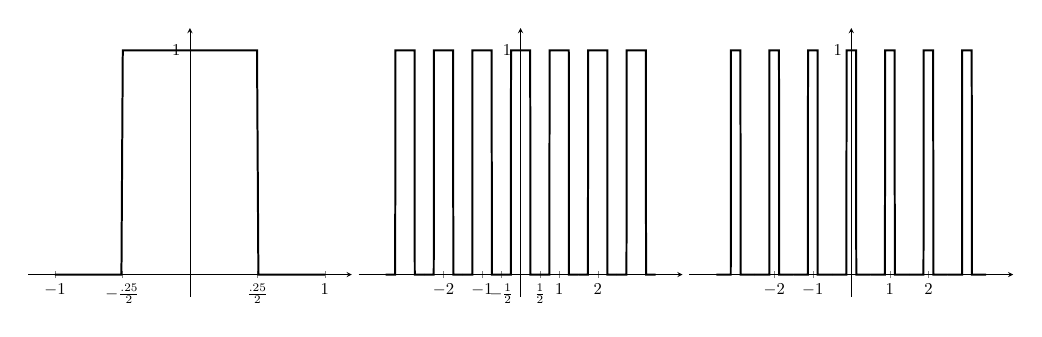
\begin{tikzpicture}[scale=.6]
\begin{scope}\begin{axis}[axis lines=middle,no markers,enlargelimits,xtick={-1,-.5,0,.5,1},xticklabels={$-1$,$-\frac{\tau}{2}$,$0$,$\frac{\tau}{2}$,$1$},ytick={0,1}]
\addplot [very thick,samples=200,domain=-1:1]  {abs(x)<.5?1:0};
\end{axis}\end{scope}
\begin{scope}[xshift=7cm]\begin{axis}[axis lines=middle,no markers,enlargelimits,xtick={-2,-1,-.5,0,.5,1,2},xticklabels={$-2$,$-1$,$-\frac{1}{2}$,0,$\frac{1}{2}$,$1$,$2$},ytick={0,1}]
\def\_tau{.5}
\def\T{1}
\foreach \n in {-3,-2,-1,0,1,2,3}
\addplot [very thick,samples=200,domain=\T*\n-\T/2:\T*\n+\T/2]  {abs(x-\n*\T)<\_tau/2?1:0};
\end{axis}\end{scope}
\begin{scope}[xshift=14cm]\begin{axis}[axis lines=middle,no markers,enlargelimits,xtick={-2,-1,0,1,2},ytick={0,1}]
\def\tau{.25}
\def\T{1}
\foreach \n in {-3,-2,-1,0,1,2,3}
\addplot [very thick,samples=200,domain=\T*\n-\T/2:\T*\n+\T/2]  {abs(x-\n*\T)<\tau/2?1:0};
\end{axis}\end{scope}
\end{tikzpicture}
\end{center}
\caption{Segnale rettangolare e onde quadre con \emph{duty cycle} del 50\% e 25\%}
\end{figure}

\subsection{Delta di Dirac}\index{segnale!impulso}
Il segnale rettangolare $\frac{1}{T} \rect{\frac{1}{T}}$ di base T e altezza 1/T ha area unitaria. Portando al limite $T\to 0$ il rettangolo diventa un impulso. Non una funzione in senso proprio ma una distribuzione integrabile chiamata \textsc{delta di Dirac}: \[\delta(t)=\lim\limits_{T\to 0}\frac{1}{T}\rect{\frac{1}{T}}\]

\subsubsection{Proprietà dell'impulso}
\begin{enumerate}
\item il segnale impulso ha area unitaria \[ \intinf{\impulse(t)}{t}=1 \]
\item il segnale impulso è funzione pari \[ \impulse(t)=\impulse(-t) \]
\item estrazione di un campione da un segnale $s(t)$ con un impulso in $t=\tau$ \[ \intinf{s(t)\impulse(t-\tau)}{t}=s(\tau) \]
è equivalente ad un impulso in $\tau$ di area $s(\tau)$
\begin{align*}
 s(t)\impulse(t-\tau)=s(\tau)\impulse(t-\tau) &\implies \\ & \intinf{s(t)\impulse(t-\tau)}{t} =\intinf{s(\tau)\impulse(t-\tau)}{t} = s(\tau)\intinf{\impulse(t-\tau)}{t} = s(\tau)
 \end{align*}
 
\item rappresentazione di un segnale come somma di infiniti impulsi
\[s(t)=\intinf{s(\tau)\impulse(t-\tau)}{\tau}=s(t)\ast\impulse(t)\]
\item derivata dell'impulso (\textsc{doppietto}) $\impulse'(t)$
\[ \intinf{s(t)\impulse'(t-\tau)}{t}=-s'(\tau) \]
\begin{proof}[Dim.]
applico l'integrazione per parti $\int{u \diff v}=u v-\int{v\diff u}$ con $u=s(t) ,\, \diff u=s'(t)\diff t ,\, \diff v=\impulse'(t-\tau)\diff t ,\, v=\impulse(t-\tau)$  a 
\[\intinf{s(t)\impulse'(t-\tau)}{t}= \restrict{s(t)\impulse(t-\tau)}{-\infty}^{+\infty} -\intinf{\impulse(t-\tau)s'(t)}{t}=-s'(\tau)  \]
\end{proof}
\item impulso è derivata del gradino
\[\intinf{\impulse(\tau)}{\tau}=\step(t)  \to \impulse(t)=\deriv{\step(t)}{t} \]
\item scala
\[\impulse(a t+b)=\intinf{s(t)\impulse(a t+b)}{t}\]
applicando le sostituzioni $\begin{cases}x=a t+b \\ t=\frac{x-b}{a}\end{cases}$
\[\intinf{\f{s}{\frac{x-b}{a}}\impulse(x)}{\frac{x}{\abs{a}}}=\frac{1}{\abs{a}}\f{s}{-\frac{b}{a}}\]
\[\intinf{s(t)\frac{1}{\abs{a}}\f{\impulse}{t+\frac{b}{a}}}{t}=\frac{1}{\abs{a}}\f{s}{-\frac{b}{a}}\]
\[\implies\impulse(a t+b)=\frac{1}{\abs{a}}\f{\impulse}{t+\frac{b}{a}} \]

\end{enumerate}

\subsection{Segnale sinusoidale}\index{segnale!sinusoidale}
Il segnale sinusoidale di ampiezza $A$, pulsazione angolare $\omega=2\pi f$, periodo $T=\frac{2\pi}{\omega}$, frequenza $f=\frac{1}{T}$, fase iniziale $\phi$
\[s(t)=A\sen{2\pi f t+\phi} \]

Potenza media 
\[P_m=\frac{1}{T}\intd{-T/2}{T/2}{A^2\Sen^2(2\pi f t+\phi)}{t}= \frac{A^2}{2}\]

infatti essendo $\Sen^2(x)=\frac{1}{2}-\frac{1}{2}\cos{2x}$
\[\begin{split}P_m&=\frac{1}{T}\intd{-T/2}{T/2}{\left(\frac{A^2}{2}-\frac{A^2}{2}\cos{4\pi f t+2\phi}\right)}{t}=\\
&=\restrict{\frac{A^2}{2 T}}{-T/2}^{T/2}-\frac{A^2}{2 T}\underbrace{\intd{-T/2}{T/2}{\cos{4\pi f t+2\phi}}{t}}_{=0}=\frac{A^2}{2}\end{split}\]

Potenza di picco \[P_p=\max\limits_{t} A^2\Sen^2(2\pi f t+\phi)=A^2\]

Fattore di picco \[\frac{P_p}{P_m}=2\]

\subsection{Segnale seno cardinale}\index{segnale!seno cardinale}
\[\sinc{t}=\frac{\sen{\pi t}}{\pi t}\]

\begin{figure}[h!]
\centering
\subfloat[][$\sinc{t}=\frac{\sen{\pi t}}{\pi t}$]
{\begin{tikzpicture}[scale=.8]
\begin{axis}[axis lines=middle,no markers,enlargelimits,xscale=1.5,xtick={0,1,2,3,4,5,6},ytick={0,1}]
\addplot [very thick,domain=-6:6,samples=100] {sin(pi*x)/(pi*x)};
\end{axis}\end{tikzpicture}} \qquad
\subfloat[][$\sinc{\frac{t}{T}}=\frac{\sen{\frac{\pi t}{T}}}{\frac{\pi t}{T}}$]
{\begin{tikzpicture}[scale=.8]
\begin{axis}[axis lines=middle,no markers,enlargelimits,xscale=1.5,xtick={-9.424,-6.283,-3.141,0,3.141,6.283,9.424},ytick={0,1},xticklabels={$-3T$,$-2T$,$-T$,$0$,$T$,$2T$,$3T$}]
\addplot [very thick,domain=-3.1*pi:3.1*pi,samples=100] {sin(x)/x};
\end{axis}\end{tikzpicture}}
\caption{Segnale seno cardinale}
\label{fig:sinc}
\end{figure}

\chapter{Serie e trasformata di Fourier}

\section{Serie di Fourier esponenziale}
Dato un segnale periodico $s(t)$ di frequenza $f_0=\frac{1}{T}$ e periodo $T$ tale che $s(t)=s(t+k T)$, è possibile esprimerlo come somma di infinite sinusoidi pesate di frequenza multipla di $f_0$, $f_k=k f_0=\frac{k}{T}$.

\begin{definizione}
Dato il segnale periodico $s(t)=s(t+k T)$ si definisce la sua rappresentazione in \textsc{serie di Fourier} in forma di esponenziali complessi:
\begin{equation}\label{eq:serie_fourier}\index{serie!di Fourier}
s(t)=\sum_{k=-\infty}^{+\infty} c_k \e{\imath 2\pi k f_0 t}
\end{equation}
\end{definizione}
Le sinusoidi pesate sono espresse in forma di esponenziali complessi ricordando le formule di Eulero
\begin{equation}\e{\imath x}=\cos{x}+\imath\sen{x}\qquad\cos{x}=\frac{\e{\imath x}+\e{-\imath x}}{2}\qquad\sen{x}=\frac{\e{\imath x}-\e{-\imath x}}{2\imath}\end{equation}
I coefficienti $c_k$ costituiscono il peso o contributo della sinusoide a frequenza $f_k$ e si calcolano come
\begin{equation}\label{eq:serie_fourier_coef}\index{serie!di Fourier!coefficienti}
c_k=\frac{1}{T}\intd{-\frac{T}{2}}{\frac{T}{2}}{s(t)\e{-\imath 2\pi k f_0 t}}{t} 
\end{equation}
Si può verificare sostituendo $s(t)$
\[c_k=\frac{1}{T}\intd{-\frac{T}{2}}{\frac{T}{2}}{ \left[\sum_{n=-\infty}^{+\infty} c_n \e{\imath 2\pi n f_0 t}\right] \e{-\imath 2\pi k f_0 t}}{t} = \frac{1}{T}\intd{-\frac{T}{2}}{\frac{T}{2}}{ \sum_{n=-\infty}^{+\infty} c_n \e{\imath 2\pi (n-k) f_0 t} }{t} \]
ipotizzando la convergenza della serie $s(t)$ ed essendo gli operatori $\sum$ e $\int$ lineari posso invertirne l'ordine
\[\begin{split}=&\frac{1}{T}\sum_{n=-\infty}^{+\infty} c_n \intd{-\frac{T}{2}}{\frac{T}{2}}{\e{\imath 2\pi(n-k)f_0 t}}{t}
=\frac{1}{T}\sum_{n=-\infty}^{+\infty} c_n \bound{-\frac{T}{2}}{\frac{T}{2}}{\frac{\e{\imath 2\pi(n-k)\frac{1}{T}t}}{\imath 2\pi(n-k)\frac{1}{T} }}\\
=&\frac{1}{T}\sum_{n=-\infty}^{+\infty} c_n T \frac{\e{\imath \pi(n-k)}-\e{-\imath\pi(n-k)}}{2\imath\pi(n-k)}
=\sum_{n=-\infty}^{+\infty} c_n \frac{\sen{\pi(n-k)}}{\pi(n-k)}
=\sum_{n=-\infty}^{+\infty} c_n \sinc{n-k} = c_k 
\end{split}\]
essendo definito il $\sinc{x}=\frac{\sen{\pi x}}{\pi x}$, si ha che sinusoidi a frequenza diversa risultano ortogonali tra loro ovvero $\sinc{n-k}=\begin{cases}
1 & n=k \\ 0 & n\neq k\end{cases}$, l'integrale sul periodo del prodotto da contributo nullo e la sommatoria per $n$ si riduce al solo contributo per $n=k$.

I coefficienti $c_k$ sono numeri complessi $c_k=\abs{c_k}\e{\imath\theta_k}$ con ampiezza e fase associati alla armonica di frequenza $f_k$.

Il coefficiente $c_0$ corrispondente alla frequenza nulla si dice \textsc{componente continua} del segnale ed è pari al valor medio del segnale periodico in un periodo:
\begin{equation}c_0=\frac{1}{T}\intd{-\frac{T}{2}}{\frac{T}{2}}{s(t)}{t} \end{equation}

\begin{nota}Nei sistemi reali è sempre presente rumore per cui i termini $c_k$ ad un certo punto non danno contributi utili ad alte frequenze quindi posso sommare un numero finito di termini $c_0 + c_1\e{\imath 2\pi f_0 t}+c_{-1}\e{-\imath 2\pi f_0 t}+\dots\approx s(t)$.\end{nota}

\section{Condizioni di esistenza Dirichlet}\index{serie!di Fourier!condizioni Dirichlet}
Perché converga lo sviluppo in serie di Fourier del segnale $s(t)$ sono sufficienti le seguenti condizioni di esistenza:
\begin{enumerate}
\item $s(t)$ sia assolutamente integrabile in un periodo: $\intd{0}{T}{\abs{(s(t)}}{t}<+\infty$
\item $s(t)$ abbia nel periodo un numero finito di massimi e minimi
\item $s(t)$ abbia nel periodo un numero finito di discontinuità di I specie\footnote{Esistono finiti $\lim\limits_{t\to t_0+}s(t)\neq\lim\limits_{t\to t_0-}s(t)$, discontinuità I specie eliminabile $s(t_0)=\frac{s(t_0^+)-s(t_0^-)}{2}$}
\end{enumerate}
\begin{nota}Le condizioni sono molto restrittive ai fini pratici, anche segnali elementari come l'impulso e il gradino non ammettono sviluppo in serie di Fourier sotto tali condizioni.\end{nota}

\section{Serie di Fourier di sinusoidi}
Lo sviluppo in serie di Fourier può essere espresso come serie somma di seni e coseni o sinusoidi
\[\begin{split} s(t)&=\sum_{k=0}^{+\infty}\left[ a_k \sen{2\pi\frac{k}{T}t} + b_k \cos{2\pi\frac{k}{T}t}\right] \\
&=\sum_{k=0}^{+\infty}A_k\left[\sen{2\pi\frac{k}{T}t+\phi_k}\right] =\sum_{k=0}^{+\infty}A_k\left[\sen{2\pi\frac{k}{T}t}\Cos\phi_k +\cos{2\pi\frac{k}{T}t}\Sen\phi_k \right]
\end{split}\]
dove $a_k,b_k \in\R,\,\begin{cases}a_k=A_k\Cos\phi_k \\b_k=A_k\Sen\phi_k \end{cases}\implies\begin{cases}A_k^2=a_k^2+b_k^2\\ \tg\phi_k=\frac{b_k}{a_k} \end{cases}\implies\begin{cases}A_k=\sqrt{a_k^2+b_k^2}\\ \phi_k=\arctg\frac{b_k}{a_k} (+\pi\text{ se }a_k<0) \end{cases}$ 

I coefficienti $a_k$ e $b_k$ si calcolano come
\[a_k=\frac{2}{T}\intd{-\frac{T}{2}}{+\frac{T}{2}}{s(t)\sen{2\pi\frac{k}{T}t}}{t} \qquad b_k=\frac{2}{T}\intd{-\frac{T}{2}}{+\frac{T}{2}}{s(t)\cos{2\pi\frac{k}{T}t}}{t}\]
che per $k=0$ si semplificano nei coefficienti $a_0=0 \quad b_0=\frac{1}{T}\intd{0}{T}{s(t)}{t}$

\section{Equivalenza tra serie di Fourier}
Si dimostra che le serie di Fourier espresse come somma di esponenziali complessi e come somma di sinusoidi sono equivalenti.

\begin{proof}[Dim.]
\[s(t)=\sum_{k=-\infty}^{+\infty} c_k \e{\imath 2\pi\frac{k}{T}t} = \sum_{k=0}^{+\infty}\left[ a_k \sen{2\pi\frac{k}{T}t} + b_k \cos{2\pi\frac{k}{T}t}\right] 
\]

Si vede che $\qquad b_0=c_0 \qquad b_k=c_k+c_{-k} \qquad a_k=\imath (c_k-c_{-k})$

Infatti si può scrivere
\[\begin{split}\sum_{k=-\infty}^{+\infty} & c_k \e{\imath 2\pi\frac{k}{T}t} = c_0+ \sum_{k=1}^{+\infty} \left[ c_k \e{\imath 2\pi\frac{k}{T}t} + c_{-k} \e{-\imath 2\pi\frac{k}{T}t} \right] = \\
&= c_0 + \sum_{k=1}^{+\infty} {\left\lbrace c_k \left[\cos{2\pi\frac{k}{T}t}+\imath\sen{2\pi\frac{k}{T}t}\right]
+c_{-k}\left[\cos{2\pi\frac{k}{T}t}-\imath\sen{2\pi\frac{k}{T}t}\right] \right\rbrace}=\\
&= c_0 + \sum_{k=1}^{+\infty} {\left[(c_k+c_{-k}) \cos{2\pi\frac{k}{T}t}+
(c_k-c_{-k})\imath\sen{2\pi\frac{k}{T}t}\right] }\end{split}\]
\end{proof}

\[b_k=c_k+c_{-k}=\frac{1}{T}\intd{-\frac{T}{2}}{\frac{T}{2}}{s(t)\left[\e{\imath 2\pi\frac{k}{T}t}+\e{-\imath 2\pi\frac{k}{T}t}\right]}{t}=\frac{2}{T}\intd{-\frac{T}{2}}{\frac{T}{2}}{s(t)\cos{2\pi\frac{k}{T}t}}{t} \]
\[a_k=\imath(c_k-c_{-k})=\imath\frac{1}{T}\intd{-\frac{T}{2}}{\frac{T}{2}}{s(t)\left[\e{\imath 2\pi\frac{k}{T}t}-\e{-\imath 2\pi\frac{k}{T}t}\right]}{t}=\frac{2}{T}\intd{-\frac{T}{2}}{\frac{T}{2}}{s(t)\sen{2\pi\frac{k}{T}t}}{t} \]

\begin{nota}L'informazione del segnale è contenuta nei pesi $c_k$ o equivalentemente $a_k$ e $b_k$.
\end{nota}

\section{Simmetrie coefficienti}
Per un segnale reale $s(t)\in\R$ la parte immaginaria deve essere nulla ovvero i termini $c_k=\Re c_k + \imath \Im c_k$ devono essere tali che $c_k \e{\imath 2\pi\frac{k}{T}t}+ c_{-k}\e{-\imath 2\pi\frac{k}{T}t}\in\R,\forall k$ 
\[c_k+c_{-k}\in\R \implies \Im c_k+\Im c_{-k}=0 \implies \Im c_k=-\Im c_{-k}\]
\[c_k-c_{-k} \text{ immaginario puro } \implies \Re c_k -\Re c_{-k}=0 \implies \Re c_k=\Re c_{-k} \]

Per un segnale reale quindi i coefficienti sono complessi e coniugati $c_k=\conj{c_{-k}}$ (\textsc{simmetria Hermitiana})

Per un segnale reale e pari si ha $a_k=0\,\forall k \implies c_k=c_{-k}$ 

Per un segnale reale e dispari si ha $b_k=0\,\forall k \implies c_k=-c_{-k}$

\section{Esempio serie di Fourier di un'onda quadra}
\begin{esempio}
Segnale onda quadra di periodo T durata $\tau$ in fig.\ref*{fig:onda_quadra} \[s(t)=\sum_{n=-\infty}^{+\infty}\rect{\frac{t-n T}{\tau}}\]

\begin{figure}[ht]
\begin{center}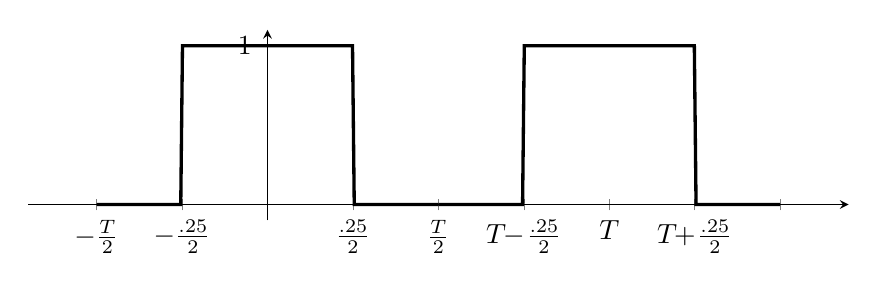
\begin{tikzpicture}
	\begin{axis}[width=12cm, height=4cm, axis lines=middle,no markers,enlargelimits,xtick={-1,-.5,0,.5,1,1.5,2,2.5,3},xticklabels={$-\frac{T}{2}$,$-\frac{\tau}{2}$,$0$,$\frac{\tau}{2}$,$\frac{T}{2}$,$T\!\!-\!\frac{\tau}{2}$,$T$,$T\!\!+\!\frac{\tau}{2}$},ytick={0,1}]
	\addplot [very thick,samples=200,domain=-1:1]  {abs(x)<.5?1:0};
	\addplot [very thick,samples=200,domain=1:3]  {abs(x-2)<.5?1:0};
	\end{axis}
	\end{tikzpicture}
\end{center}
\caption{Onda quadra}\label{fig:onda_quadra}
\end{figure}
Il segnale è reale pari ($c_k=c_{-k}$), i coefficienti della serie di Fourier si calcolano applicando la formula \ref{eq:serie_fourier_coef}:
\[\begin{split}c_k&=\frac{1}{T}\intd{-\frac{T}{2}}{\frac{T}{2}}{s(t)\e{-\imath 2\pi\frac{k}{T}t}}{t}
=\frac{1}{T}\intd{-\frac{T}{2}}{\frac{T}{2}}{\e{-\imath 2\pi\frac{k}{T}t}}{t}
=\frac{1}{T}\bound{-\frac{\tau}{2}}{\frac{\tau}{2}}{ \frac{\e{-\imath 2\pi\frac{k}{T}t}}{-\imath 2\pi\frac{k}{T}}}=\\
&=\frac{1}{\pi k} \frac{-\e{-\imath 2\pi\frac{k}{T}\frac{\tau}{2}}+\e{\imath 2\pi\frac{k}{T}\frac{\tau}{2}}}{\imath 2} 
=\frac{\sen{\pi \tau \frac{k}{T}}}{\pi k}
=\frac{\tau}{T}\frac{\sen{\pi k \frac{\tau}{T}}}{\pi k \frac{\tau}{T}} 
=\frac{\tau}{T}\sinc{k \frac{\tau}{T}}
\end{split}\]

\begin{figure}[h!]
\centering
{\begin{tikzpicture}[scale=.6]
	\begin{axis}[width=10cm,axis lines=middle,no markers,enlargelimits,xscale=1.5,xtick={-3,-1,0,1,3},xticklabels={$-T$,$-\tau$,0,$\tau$,$T$},ytick={0,1},yticklabels={0,$\frac{\tau}{T}$}]
	\addplot [dashed,domain=-7:7,samples=100] {sin(pi*x/3)/(pi*x/3)};
	\addplot+[only marks,samples at={-3,-2,-1,0.001,1,2,3}]
	{sin(pi*x/3)/(pi*x/3)};
	\end{axis}\end{tikzpicture}}
\caption{Valori coefficienti $c_k=\frac{\tau}{T}\sinc{\frac{t}{T}}$}
\label{fig:sinc_onda_quadra}
\end{figure}
\end{esempio}

\section{Proprietà della serie di Fourier}
\subsection{Linearità}L'integrale è un operatore lineare pertanto una combinazione lineare di segnali trasforma linearmente i coefficienti della serie
\[ y(t)=a s_1(t)+ b s_2(t)\]  
\[ c_{y k}= a c_{1 k} + b c_{2 k} \]

\subsection{Traslazione nel tempo}
Un segnale traslato nel tempo $s(t-\tau)$, ritardato o anticipato di un tempo $\tau$, vede i coefficienti modificati nella fase $c_r^{'}=c_k \e{-\imath 2\pi\frac{k}{T}\tau}$

\begin{proof}[Dim.]
\[ \intd{-\frac{T}{2}}{\frac{T}{2}}{s(t-\tau)\e{-\imath 2\pi\frac{k}{T}t}}{t} \]
effettuando il cambio di variabile $t-\tau=x$, $t=x+\tau$, $\diff t=\diff x$
\[\intd{-\frac{T}{2}}{\frac{T}{2}}{s(x)\e{-\imath 2\pi\frac{k}{T}x}\e{-\imath 2\pi\frac{k}{T}\tau}}{x} =
\e{-\imath 2\pi\frac{k}{T}\tau} \intd{-\frac{T}{2}}{\frac{T}{2}}{s(x)\e{-\imath 2\pi\frac{k}{T}x}}{x}\]
si nota anche che data la periodicità per $\tilde{\tau}=\tau+N T$
\[\e{-\imath 2\pi\frac{k}{T}\tilde{\tau}}=
\e{-\imath 2\pi\frac{k}{T}\tau} \underbrace{\e{-\imath 2\pi\frac{k}{T}N T}}_{1}=\e{-\imath 2\pi\frac{k}{T}\tau}
\]
\end{proof}

\section{Potenza segnale periodico (Teo. Parseval)}
La potenza del segnale periodico è contenuta nei suoi toni armonici:
\begin{equation}\label{eq:teo_Parseval}\index{Teorema!Parseval}
P=\sum_{k=-\infty}^{+\infty}{\abs{c_k}^2}
\end{equation}

\begin{proof}[Dim.]
\[\begin{split}P&= \frac{1}{T}\intd{-\frac{T}{2}}{\frac{T}{2}}{\abs{s(t)}^2}{t}=\frac{1}{T}\intd{-\frac{T}{2}}{\frac{T}{2}}{ \left(\sum_{k=-\infty}^{+\infty}{c_k\e{\imath 2\pi\frac{k}{T}t}}\right) \left(\sum_{n=-\infty}^{+\infty}{c_n\e{\imath 2\pi\frac{n}{T}t}}\right)}{t}= \\
&=\frac{1}{T}\intd{-\frac{T}{2}}{\frac{T}{2}}{ \left(\sum_{k=-\infty}^{+\infty}{c_k\e{\imath 2\pi\frac{k}{T}t}}\right) \left(\sum_{n=-\infty}^{+\infty}{\conj{c_n}\e{-\imath 2\pi\frac{n}{T}t}}\right)}{t}= \\
\intertext{il prodotto di armoniche ortogonali da contributo non nullo solo per $n=k$, pertanto}
&=\frac{1}{T}\intd{-\frac{T}{2}}{\frac{T}{2}}{ \left(\sum_{k=-\infty}^{+\infty}{c_k \conj{c_k} \e{\imath 2\pi\frac{k}{T}t} \e{-\imath 2\pi\frac{k}{T}t}}\right)}{t}= \\
&=\frac{1}{T}\intd{-\frac{T}{2}}{\frac{T}{2}}{\sum_{k=-\infty}^{+\infty}{\abs{c_k}^2}}{t}=
\frac{1}{T}\sum_{k=-\infty}^{+\infty}{\abs{c_k}^2}\intd{-\frac{T}{2}}{\frac{T}{2}}{}{t}=\sum_{k=-\infty}^{+\infty}{\abs{c_k}^2}
\end{split}\]
\end{proof}

\section{Trasformata di Fourier}
Per segnali non periodici la potenza del segnale non è concentrata nei moti armonici ma è distribuita con continuità a tutte le frequenze dello spettro.

Il segnale aperiodico è rappresentabile come l'\textsc{integrale di Fourier}
\begin{equation}
s(t)=\intinf{S(f)\e{\imath 2\pi f t}}{f}
\end{equation}

La funzione complessa $S(f)$, nella variabile continua $f$, rappresenta la \textsc{trasformata di Fourie}r del segnale $s(t)$
\begin{equation}
S(f)=\intinf{s(t)\e{-\imath 2\pi f t}}{t}
\end{equation}
Il modulo e la fase della grandezza complessa definiscono
\[\abs{S(f)} \text{ spettro di ampiezza} \quad \angle S(f) \text{ spettro di fase}\]

\subsection{Condizioni di esistenza di Dirichlet}
I criteri di Dirichlet condizioni sufficienti per l'esistenza della trasformata di Fourier di un segnale $s(t)$:
\begin{enumerate}
\item $\intinf{\abs{s(t)}}{t}<\infty$ (assolutamente integrabile)
\item numero finito di discontinuità (tutte di I specie)
\item numero finito di max e min
\end{enumerate}
\begin{nota}Le condizioni non sono necessarie: alcune funzioni pur non soddisfacendo le tre condizioni sono trasformabili.\end{nota}
\begin{esempio}
Il segnale aperiodico di durata limitata $\tau$ ha trasformata di Fourier
\[s(t)=\rect{\frac{t}{\tau}}\quad\fourier{\rect{\frac{t}{\tau}}}=\tau\sinc{f\tau} \]

\begin{figure}[h!]
\centering
\subfloat[][$s(t)=\rect{\frac{t}{\tau}}$]
{\begin{tikzpicture}[scale=.6]
	\begin{axis}[axis lines=middle,no markers,enlargelimits,xscale=1.5,xtick={-.5,0,.5},xticklabels={$-\frac{\tau}{2}$,$0$,$\frac{\tau}{2}$},ytick={0,1}]
	\addplot [very thick,samples=200,domain=-1:1]  {abs(x)<.5?1:0};
	\end{axis}
\end{tikzpicture}}\qquad
\subfloat[][$S(f)=\tau\sinc{f\tau}$]
{\begin{tikzpicture}[scale=.6]
	\begin{axis}[axis lines=middle,no markers,enlargelimits,xscale=1.5,xtick={-9.424,-6.283,-3.141,0,3.141,6.283,9.424},ytick={0,1},xticklabels={$-3\tau$,$-2\tau$,$-\tau$,$0$,$\tau$,$2\tau$,$3\tau$},yticklabels={$0$,$\tau$}]
	\addplot [very thick,domain=-3.5*pi:3.5*pi,samples=100] {sin(x)/x};
	\end{axis}\end{tikzpicture}}
\end{figure}

\[\begin{split}S(f)&=\intinf{s(t)\e{-\imath 2\pi f t}}{t}
=\intd{-\frac{\tau}{2}}{\frac{\tau}{2}}{1\cdot\e{-\imath 2\pi f t}}{t}
=\bound{-\frac{\tau}{2}}{\frac{\tau}{2}}{\frac{\e{-\imath 2\pi f t}}{-\imath 2\pi f}}=\\
&=\frac{-\e{-\imath 2\pi f\frac{\tau}{2}}+\e{\imath 2\pi f\frac{\tau}{2}}}{\imath 2\pi f} 
=\tau\frac{\sen{\pi f\tau}}{\pi f\tau}
=\tau\sinc{f\tau}
\end{split}\]
\end{esempio}

\section{Proprietà trasformata di Fourier}
\subsection{Simmetria}
La trasformata di un segnale reale $s(t)$ gode di simmetria hermitiana $\conj{S}(f)=S(-f)$
\begin{equation}\conj{S}(f)=\intinf{s(t)\e{+\imath 2\pi f t}}{t}=S(-f)\end{equation}
Espresso nella parte reale e immaginaria
\[S(f)=S_R(f)+\imath S_I(f)=\intinf{s(t)\cos{2\pi f t}}{t}-\imath\intinf{s(t)\sen{2\pi f t}}{t}\]
Se $s(t)$ è reale pari, la trasformata è reale pari: \[\conj{S}(f)=\conj{[S_R(f)]}=S(-f)\] \[S_R(f)=S_R(-f)\]
Se $s(t)$ è reale dispari, la trasformata è immaginaria pura dispari:
\[\conj{S}(f)=\conj{[+\imath S_I(f)]}=-\imath S_I(f)=\imath S_I(-f)\] \[S_I(f)=-S_I(-f)\]

\subsection{Linearità}
La trasformata di Fourier di combinazione lineare di segnali gode di linearità
\begin{equation}
\fourier{a x(t)+ b y(t)}= a X(f)+ b Y(f)
\end{equation}

\begin{proof}[Dim.]
Applicando la definizione di trasformata e per la linearità dell'operatore integrale
\[ \intinf{\left[a x(t)+ b y(t)\right]\e{-\imath 2\pi f t}}{t}= a\intinf{x(t)\e{-\imath 2\pi f t}}{t} + b\intinf{y(t)\e{-\imath 2\pi f t}}{t}= a X(f) + b Y(f) \]
\end{proof}

\subsection{Traslazione nel tempo}
La trasformata di Fourier di un segnale anticipato o ritardato nel tempo modifica lo spettro di fase del segnale
\begin{equation}
\fourier{s(t-\tau)}= S(f)\e{-\imath 2\pi f \tau}
\label{eq:trasf_Fourier_trasl}
\end{equation}
\begin{proof}[Dim.]
Applicando un cambio di variabile $\alpha=t-\tau$ e la definizione di trasformata
\[\intinf{s(t-\tau)\e{-\imath 2\pi f t}}{t}=
\intinf{s(\alpha)\e{-\imath 2\pi f\alpha}\e{-\imath 2\pi f\tau}}{\alpha}=S(f)\e{-\imath 2\pi f\tau}\]
\end{proof}

\subsection{Ribaltamento}
La trasformata di Fourier di un segnale invertito nel tempo ha lo spettro del segnale ribaltato nelle frequenze
\begin{equation}\fourier{s(-t)}=S(-f)\end{equation}
\begin{proof}[Dim.]
Applicando un cambio di variabile $\alpha=-t$ e la definizione di trasformata
\[\intinf{s(-t)\e{-\imath 2\pi f t}}{t}=
\intinf{s(\alpha)\e{-\imath 2\pi (-f)\alpha}}{\alpha}=S(-f)\]
\end{proof}

\subsection{Cambiamento di scala temporale}
La trasformata di Fourier di un segnale compresso o dilatato nella scala dei tempi dilata o comprime lo spettro delle frequenze del segnale
\begin{equation}\label{eq:trasf_Fourier_scala}
\fourier{s(a t)}=\frac{1}{\abs{a}}\,\f{S}{\frac{f}{a}}
\end{equation}
\begin{proof}[Dim.] Applicando un cambio di variabile $\alpha=a t, t=\frac{\alpha}{a}, \diff t=\frac{\diff\alpha}{a}$ e la definizione di trasformata
\[\intinf{s(a t)\e{-\imath 2\pi f t}}{t}=
\int_{-\infty}^{\infty}{s(\alpha)\e{-\imath 2\pi\frac{f}{a}\alpha}}{\frac{\diff\alpha}{\abs{a}}}=\frac{1}{\abs{a}}\,\f{S}{\frac{f}{a}}\]
\end{proof}

\subsection{Derivazione}
La trasformata di Fourier della derivata di un segnale 
\begin{equation}
\fourier{s'(t)}=\imath 2\pi f\,S(f)
\end{equation}
\begin{proof}[Dim.] Si ha infatti che per un segnale derivabile $s(t)$
\[s(t)=\intinf{S(f)\e{\imath 2\pi f t}}{f}\implies s'(t)=\deriv{}{t}\intinf{S(f)\e{\imath 2\pi f t}}{f}=
\intinf{ \underbrace{\imath 2\pi f S(f)}_{\fourier{s'(t)}}\e{\imath 2\pi f t}}{f} \]
\end{proof}

\begin{nota}L'operatore derivata temporale di un segnale si comporta come un filtro passa alto perché nelle frequenze si ha il prodotto con il fattore $\imath 2\pi f$ che essendo proporzionale alla frequenza $f$ esalta in modulo le alte frequenze, mentre attenua le frequenze per $f\to 0$. La fase viene modificata di $\pm\frac{\pi}{2}$ a seconda del segno di $f$.\end{nota}

\subsection{Convoluzione nel tempo}
La trasformata di Fourier del prodotto di convoluzione di due segnali
\begin{equation}
\fourier{x(t)\ast y(t)}=X(f)\cdot H(f)
\label{eq:trasf_Fourier_conv}
\end{equation}
\begin{proof}[Dim.] Applicando la trasformata di Fourier al prodotto di convoluzione e l'eq.\ref{eq:trasf_Fourier_trasl}
\[\begin{split}& \intinf{ \left[\intinf{x(\tau)h(t-\tau)}{\tau}\right] \e{-\imath 2\pi f t}}{t} = 
\intinf{ x(\tau) \left[\intinf{h(t-\tau)\e{-\imath 2\pi f t}}{t}\right]}{\tau}=\\
=& \intinf{ x(\tau) H(f)\e{-\imath 2\pi f \tau}}{\tau} = X(f) H(f) \end{split}\]
\end{proof}

\subsection{Dualità}
Nota la trasformata di Fourier $S(f)$ di un segnale $s(t)$ si ha che la trasformata di Fourier del segnale temporale $S(t)$ è per dualità $s(-f)$
\begin{equation}
\begin{split}
s(t) &\overset{\Fourier}{\to} S(f) \\
S(t) &\overset{\Fourier}{\to} s(-f)
\end{split}
\end{equation}
\begin{proof}[Dim.]
Nella tra il segnale e la sua trasformata $s(t)=\intinf{S(f)\e{+\imath 2\pi f t}}{f}$
si ha scambiando formalmente le variabili $t$ e $f$ \[s(f)=\intinf{S(t)\e{+\imath 2\pi f t}}{t}\]
cambiando variabile $f$ con $-f$
\[\fourier{S(t)}=\intinf{S(t)\e{-\imath 2\pi f t}}{t}=s(-f)\]
\end{proof}

\begin{esempio}
\begin{equation}
\begin{split}
\rect{t} &\overset{\Fourier}{\to} \sinc{f}\\
\sinc{t} &\overset{\Fourier}{\to} \rect{-f}=\rect{f}
\end{split}
\end{equation}
La proprietà di dualità consente di ottenere velocemente risultati che richiederebbero molti calcoli applicando la definizione.
\end{esempio}

\begin{esempio}\label{es:trasf_Fourier_conv}
	
\begin{figure}[h!]
\centering
\subfloat[][$s(t)=\rect{\frac{t}{T}}\ast\rect{\frac{t}{T}}$]
{\begin{tikzpicture}[scale=.67]
\begin{axis}[axis lines=middle,no markers,enlargelimits,xscale=1.2,xtick={-1,0,1},ytick={0,1},xticklabels={$-T$,0,$T$},yticklabels={0,$T$}]
\addplot [very thick]coordinates {(-2,0)(-1,0)(0,1)(1,0)(2,0)};
\end{axis}\end{tikzpicture}}\qquad
\subfloat[][$S(f)=T^2\Sinc^2(f T)$] {
\begin{tikzpicture}[scale=.7]
\begin{axis}[axis lines=middle,no markers,enlargelimits,xscale=1.5,xtick={-9.424,-6.283,-3.141,0,3.141,6.283,9.424},ytick={0,1},xticklabels={$-\frac{3}{T}$,$-\frac{2}{T}$,$-\frac{1}{T}$,$0$,$\frac{1}{T}$,$\frac{2}{T}$,$\frac{3}{T}$},yticklabels={$0$,$T^2$}]
\addplot [very thick,domain=-3.5*pi:3.5*pi,samples=100] { (sin(x)/x)^2 };
\end{axis}\end{tikzpicture}	
}
\caption{Esempio \ref{es:trasf_Fourier_conv} convoluzione segnali rettangolari e trasformata}
\end{figure}

\[s(t)=\rect{\frac{t}{T}}\ast\rect{\frac{t}{T}}\]
Per la prop. di scala $\rect{\frac{t}{T}}\overset{\Fourier}{\to}T\sinc{f T}$ e per la prop. di convoluzione si ha
\[S(f)=T^2\Sinc^2(f T)\]
\end{esempio}

\subsection{Traslazione in frequenza}
L'anti-trasformata di Fourier del segnale traslato in frequenza $S(f-f_0)\overset{\Fourier^{-1}}{\rightarrow}s(t)\e{\imath 2\pi f_0 t}$

\begin{proof}[Dim.]
Applicando l'anti trasformata di Fourier allo spettro traslato in frequenza, con opportuno cambio di variabile $\alpha=f-f_0, f=f_0+\alpha, \diff\alpha=\diff f$
\[\intinf{S(f-f_0)\e{\imath 2\pi f t}}{f}=
\intinf{S(\alpha)\e{\imath 2\pi\alpha t}\e{\imath 2\pi f_0 t}}{\alpha}=\e{\imath 2\pi f_0 t} s(t) \]
\end{proof}

\subsection{Prodotto nel tempo $\to$ convoluzione in frequenza}
Dati due segnali $x(t)$ e $y(t)$ con le loro trasformate di Fourier $X(f)$ e $Y(f)$. La trasformata del segnale prodotto
\begin{equation}
\begin{split}
z(t) = x(t) y(t) &\overset{\Fourier}{\rightarrow} Z(f) = X(f)\ast Y(f)
\end{split}
\end{equation}

\begin{proof}[Dim.] Applicando la definizione
\[\begin{split}Z(f)&=\intd{t=-\infty}{+\infty}{z(t)\e{-\imath 2\pi f t}}{t}=\intd{t=-\infty}{+\infty}{x(t)y(t)\e{-\imath 2\pi f t}}{t}=\\
\intertext{sostituendo a $x(t)$ la sua espressione come integrale di Fourier}
&=\intd{t=-\infty}{+\infty}{\left[\intd{\nu=-\infty}{+\infty}{X(\nu)\e{\imath 2\pi\nu t}}{\nu}\right]y(t)\e{-\imath 2\pi f t}}{t}=\\
\intertext{invertendo l'ordine di integrazione}
&=\intd{\nu=-\infty}{+\infty}{X(\nu)\left[\intd{t=-\infty}{+\infty}{y(t)\e{-\imath 2\pi(f-\nu)t}}{t}\right]}{\nu}=\\
\intertext{si ha nella parentesi quadra la trasformata di $y(t)$ calcolata alla frequenza $f-\nu$}
&=\intd{\nu=-\infty}{+\infty}{X(\nu)Y(f-\nu)}{\nu} = X(f)\ast Y(f)
\end{split}\]
\end{proof}

\begin{nota}
Dato un segnale generico è possibile estrarre una finestra di durata limitata moltiplicando il segnale per un $\Rect$. Per la proprietà della trasformata del prodotto risulta che un segnale di durata limitata ha sempre banda a tutte le frequenze perché il $\Rect$ ha spettro infinito. 
\end{nota}

\subsection{Teorema di Parseval}
Per i segnali di energia finita si può sempre calcolare la trasformata di Fourier. Per il teorema di Parseval
\begin{equation}E_s=\intinf{\abs{s(t)}^2}{t}=\intinf{\abs{S(f)}^2}{f}\label{eq:parseval}\end{equation}
che da indicazioni su come è distribuita l'energia del segnale alle varie frequenze. Per l'integrale di Fourier $s(t)=\intinf{S(f)\e{\imath 2\pi f t}}{t}$ il segnale $s(t)$ è la somma di infinite sinusoidi pesate da $S(f)$: che è anche l'integrale dei contributi infinitesimi di energia alle varie frequenze dello spettro.
\begin{nota}\`{E} importante notare che per la trasformata di Fourier cambiare l'energia ad una frequenza $f_0$ non comporta cambiamenti ad altre frequenze.\end{nota}
\begin{proof}[Dim.]
\[\begin{split}\intinf{\abs{s(t)}^2}{t}&=\intinf{s(t)\conj{s}(t)}{t}
=\intinf{s(t)\conj{\left[\intinf{S(f)\e{\imath 2\pi f t}}{f}\right]}}{t}=\\
&=\intinf{s(t)\intinf{\conj{S}(f)\e{-\imath 2\pi f t}}{f}}{t}=\intinf{\conj{S}(f)\intinf{s(t)\e{-\imath 2\pi f t}}{t}}{f}=\\
&=\intinf{\conj{S}(f)S(f)}{f}=\intinf{\abs{S(f)}^2}{f}\end{split}\]
\end{proof}

\begin{nota}Tutte le proprietà della trasformata di Fourier valgono sotto le condizioni di Dirichlet. Tali condizioni sono molto stringenti ai fini pratici, anche segnali elementari come l'impulso e il gradino non ammettono trasformata di Fourier. Le condizioni saranno superate con la trasformata generalizzata.\end{nota}

\subsection{Trasformata funzione generalizzata $\delta(t)$}
Per calcolare la trasformata di Fourier della funzione generalizzata delta di Dirac $\delta(t)$ si applica la definizione tenendo conto della proprietà campionatrice della $\delta(t)$
\begin{equation}
\fourier{\delta(t)}=\intinf{\delta(t)\e{-\imath 2\pi f t}}{t}=\restrict{\e{-\imath 2\pi f t}}{t=0}=1
\end{equation}
Da questo risultato per la funzione generalizzata e per il teorema di dualità è possibile calcolare la trasformata di Fourier del segnale ad energia infinita come il segnale costante
\begin{equation}
\fourier{1}=\delta(-f)=\delta(f)
\end{equation}
\[\fourier{c}=c\,\delta(f)\]

\subsection{Trasformata funzione generalizzata $\step(t)$}
La trasformata di Fourier della funzione gradino unitario ideale $\step(t)$ non esiste. Bisogna far ricorso alla trasformata con le funzioni generalizzate, definendo il gradino come
\[\step(t)=\frac{1}{2}+\frac{1}{2}\sgn(t)\] 
\begin{equation}
\fourier{\step(t)}=\frac{1}{2}\delta(f)+\frac{1}{\imath 2\pi f}
\end{equation}
\begin{figure}[h!]\centering
\begin{tikzpicture}[scale=.6]
\begin{axis}[axis lines=middle,no markers,enlargelimits,xscale=1.5,xtick={-1,0,1},ytick={0,.5,1},yticklabels={$0$,$\frac{1}{2}$,$1$}]
\addplot [very thick]coordinates {(-1,0)(0,0)};
\addplot [only marks, samples at={0}]coordinates {(0,.5)};
\addplot [very thick]coordinates {(0,1)(1,1)};
\end{axis}\end{tikzpicture}
\caption{Funzione $\sgn(t)$}
\end{figure}

\begin{proof}[Dim.]
La trasformata della funzione $\sgn(t)$ si ottiene per dualità della trasformata della funzione $\frac{1}{t}\overset{\Fourier}{\to}-\imath\pi\sgn(f)$
\[\begin{split}&\fourier{\frac{1}{t}}=\intinf{\frac{1}{t}\e{-\imath 2\pi f t}}{t}= \underbrace{\intinf{\frac{1}{t}\cos{2\pi f t}}{t}}_{\stackrel{=0}{1/t \text{ dispari}}} -\imath\intinf{\frac{1}{t}=\sen{2\pi f t}}{t}=\\
&=-\imath 2\pi f\intinf{\frac{\sen{2\pi f t}}{2\pi f t}}{t}=-\imath 2\pi f\intinf{\sinc{2 f t}}{t}= -\imath\frac{2\pi f}{2\abs{f}} = -\imath\pi\sgn(f)
\end{split} \]
L'integrale nel tempo da $-\infty$ a $+\infty$ di un segnale è pari alla trasformata del segnale calcolata per $f=0$. La trasformata del $\sinc{t}\overset{\Fourier}{\to}\rect{f}$ per la prop. di dualità, la trasformata di $\sinc{2\alpha t}\overset{\Fourier}{\to}\frac{1}{2\abs{\alpha}}\rect{\frac{f}{2\alpha}}$ per la prop. di scala, calcolata per $f=0$ il $\rect{0}=1$, da cui 
$\intinf{\sinc{2 f t}}{t}=\frac{1}{2\abs{f}}$.

Da $s(t)=\frac{1}{t}\overset{\Fourier}{\to} -\imath\pi\sgn(f)$, per dualità $S(t)\overset{\Fourier}{\to} s(-f)$ da cui \[\fourier{\sgn(t)}=\frac{1}{-\imath\pi}\frac{1}{-f}=\frac{1}{\imath\pi f}\] da cui il risultato per la trasformata generalizzata del gradino \[\fourier{\step(t)}]=\fourier{\frac{1}{2}+\frac{1}{2}\sgn(t)}=\frac{1}{2}\delta(f)+\frac{1}{\imath 2\pi f}\]
\end{proof}

\subsection{Teorema integrazione completo}
Per un segnale definito come integrale di convoluzione con un gradino 
\[y(t)=\intd{-\infty}{t}{x(\tau)}{\tau}=\intinf{x(\tau)\step(t-\tau)}{\tau}=x(t)\ast\step(t)\] 
si può determinare la trasformata generalizzata 
\begin{equation}
Y(f)=X(f) U(f)=\frac{1}{2} X(0) \delta(f) + \frac{X(f)}{\imath 2\pi f}
\end{equation}
che tiene conto nel primo termine della componente continua del segnale.

\subsection{Trasformate funzioni seno e coseno}
Dalla funzione generalizzata $\delta(t)\overset{\Fourier}{\rightarrow}1$ si hanno per il teo. traslazione del tempo e per il teo. dualità le trasformate di Fourier delle funzioni seno e coseno
\[\begin{split}\delta(t-t_0)&\overset{\Fourier}{\to}\e{-\imath 2\pi f t_0}\\
\e{\imath 2\pi f_0 t}&\overset{\Fourier}{\to}\delta(f-f_0)\end{split}\]
\begin{equation}
\cos{2\pi f_0 t}=\frac{\e{\imath 2\pi f_0 t}+\e{-\imath 2\pi f_0 t}}{2}\overset{\Fourier}{\to}\frac{\delta(f-f_0)+\delta(f+f_0)}{2}\end{equation}
\begin{equation}\sen{2\pi f_0 t}=\frac{\e{\imath 2\pi f_0 t}-\e{-\imath 2\pi f_0 t}}{2\imath}\overset{\Fourier}{\to}\frac{\delta(f-f_0)-\delta(f+f_0)}{2\imath}\end{equation}

\subsection{Modulazione}
Per il teorema trasformata del prodotto e la proprietà campionatrice della funzione generalizzata $\delta$ si ha il risultato notevole per cui la trasformata di un segnale modulato risulta
\begin{equation}\label{eq:fourier_modulazione_coseno}
s(t) \cos{2\pi f_0 t}\overset{\Fourier}{\to}\frac{1}{2}\left[S(f-f_0)+S(f+f_0)\right]
\end{equation}
\begin{equation}
s(t) \sen{2\pi f_0 t}\overset{\Fourier}{\to}\frac{1}{2\imath}\left[S(f-f_0)-S(f+f_0)\right]
\end{equation}

\begin{proof}[Dim.]
Si ha infatti \[\fourier{s(t)\cos{2\pi f_0 t}}=S(f)\ast\frac{1}{2}\left[\delta(f-f_0)+\delta(f+f_0)\right]\] e che \[S(f)\ast\delta(f-f_0)=\intinf{S(\nu)\delta(f-f_0-\nu)}{\nu}=S(f-f_0)\]
\end{proof}

\begin{figure}[h!]
\centering
\subfloat[][$S(f)$]
{\begin{tikzpicture}[scale=.6]
	\begin{axis}[axis lines=middle,no markers,enlargelimits,xscale=1.5,xtick={-1,0,1},ytick={1}]
	\addplot [very thick]coordinates {(-2,0)(-1,0)(0,1)(1,0)(2,0)};
	\end{axis}\end{tikzpicture}}\qquad\subfloat[][$\frac{1}{2}\left\lbrace S(f-f_0)+S(f+f_0)\right\rbrace$] {
	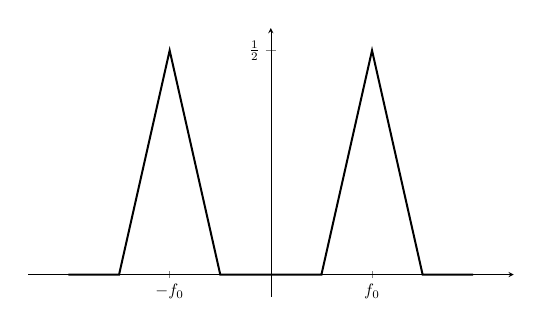
\begin{tikzpicture}[scale=.6]
	\begin{axis}[axis lines=middle,no markers,enlargelimits,xscale=1.5,xtick={-2,2},ytick={1},xticklabels={$-f_0$,$f_0$},yticklabels={$\frac{1}{2}$}]
	\addplot [very thick]coordinates {(-4,0)(-3,0)(-2,1)(-1,0)(1,0)(2,1)(3,0)(4,0)};
	\end{axis}\end{tikzpicture}	
}
\caption{Esempio modulazione}
\end{figure}

\subsection{Trasformata segnali periodici}
Un segnale periodico $s(t)$ è la somma di infinite repliche di un segnale ristretto $s_T(t)$ ad un periodo $\left[-\frac{T}{2},\frac{T}{2}\right]$ e per la definizione di serie di Fourier somma di esponenziali complessi pesati da coefficienti 
\begin{equation}
s(t)=\sum_{n=-\infty}^{+\infty}{s_T(t-n T)}=\sum_{k=-\infty}^{+\infty}{c_k\e{\imath 2\pi\frac{k}{T}t}}
\end{equation}

Definita la trasformata di Fourier del segnale ristretto $S_T(f)=\fourier{s_T(t)}$ si ha che i coefficienti 	\[c_k=\frac{1}{T}\intd{-\frac{T}{2}}{\frac{T}{2}}{s(t)\e{-\imath 2\pi\frac{k}{T}t}}{t}=\frac{1}{T}\intinf{s_T(t)\e{-\imath 2\pi\frac{k}{T}t}}{t}=\frac{1}{T}\f{S_T}{\frac{k}{T}}\]
quindi
\[s(t)=\frac{1}{T}\sum_{k=-\infty}^{+\infty}{\f{S_T}{\frac{k}{T}}\e{\imath 2\pi\frac{k}{T}t}}\]
\begin{equation}
S(f)=\frac{1}{T}\sum_{k=-\infty}^{+\infty}{\f{S_T}{\frac{k}{T}}\f{\delta}{f-\frac{k}{T}}}
\end{equation}
La trasformata di Fourier di un segnale periodico è la somma di infiniti impulsi a frequenza multipla della fondamentale.

\clearpage
\section{Esempi ed esercizi}
\begin{esempio}
La trasformata di un treno di impulsi è un treno di impulsi in frequenza
\[s(t)=\sum_{n=-\infty}^{+\infty}{\delta(t-n T)} \qquad S(f)=\frac{1}{T}\sum_{k=-\infty}^{+\infty}{\f{\delta}{f-\frac{k}{T}}}\]
\begin{nota}
Esempio importante per digitalizzazione e campionamento (par.\ref{sec:campionamento}).
\end{nota}

\begin{figure}[h!]
\centering
\subfloat[][$s(t)$]{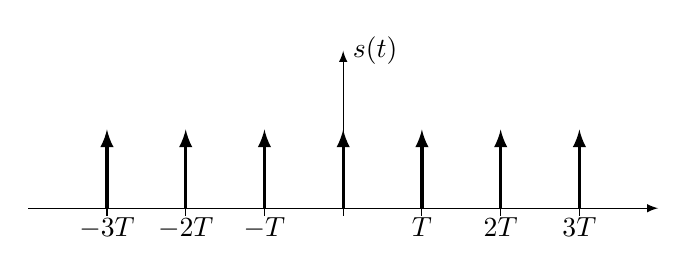
\begin{tikzpicture}
	\draw [-latex] (-4,0)--(4,0);
	\draw [-latex] (0,0)--(0,2);
	\foreach \i in {-3,...,3} 
		\draw [very thick,-latex] (\i,0)--(\i,1); 
	\foreach \i in {-3,...,3} 
		\draw (\i,0)--(\i,-1mm); 
	\node at(-3,0) [below] {$-3T$};
	\node at(-2,0) [below] {$-2T$};
	\node at(-1,0) [below] {$-T$};
	\node at(1,0) [below] {$T$};
	\node at(2,0) [below] {$2T$};
	\node at(3,0) [below] {$3T$};
	\node [right] at (0,2) {$s(t)$};
	\end{tikzpicture}
}\qquad\subfloat[][$S(f)$]{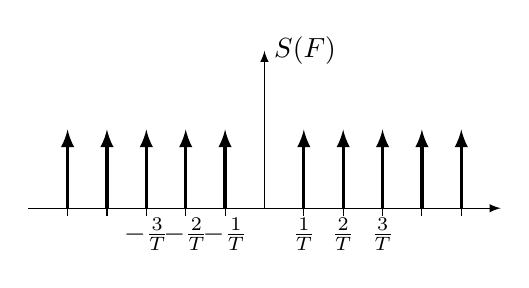
\begin{tikzpicture}
\draw [-latex] (-3,0)--(3,0);
\draw [-latex] (0,0)--(0,2);
\foreach \i in {-5,...,-1} \draw [very thick,-latex] (\i/2,0)--(\i/2,1); 
\foreach \i in {1,...,5} \draw [very thick,-latex] (\i/2,0)--(\i/2,1); 
\foreach \i in {-5,...,-1} \draw (\i/2,0)--(\i/2,-1mm);
\foreach \i in {1,...,5} \draw (\i/2,0)--(\i/2,-1mm);
\node at(-1.5,0) [below] {$-\frac{3}{T}$};
\node at(-1,0) [below] {$-\frac{2}{T}$};
\node at(-.5,0) [below] {$-\frac{1}{T}$};
\node at(.5,0) [below] {$\frac{1}{T}$};
\node at(1,0) [below] {$\frac{2}{T}$};
\node at(1.5,0) [below] {$\frac{3}{T}$};
\node [right] at (0,2) {$S(F)$};
\end{tikzpicture}}
\caption{Treno di impulsi nel tempo e in frequenza}
\end{figure}
\end{esempio}

\begin{esercizio}
Determinare la serie di Fourier del segnale onda triangolare in figura
\begin{figure}[h!]
\begin{center}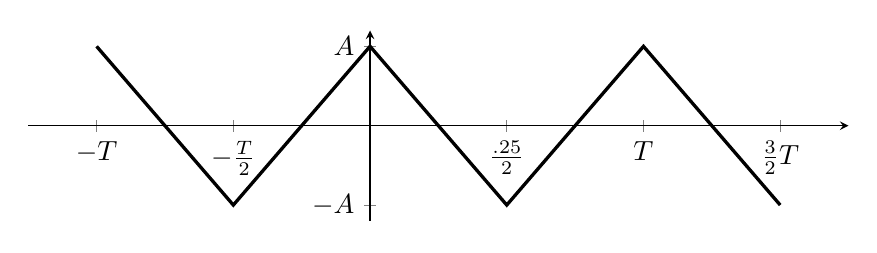
\begin{tikzpicture}
\begin{axis}[width=12cm, height=4cm, axis lines=middle,no markers,enlargelimits,xtick={-2,-1,0,1,2,3},xticklabels={$-T$,$-\frac{T}{2}$,$0$,$\frac{\tau}{2}$,$T$,$\frac{3}{2}T$},ytick={-1,0,1},yticklabels={$-A$,0,$A$}]
\addplot [very thick,domain=-2:2]coordinates {(-2,1)(-1,-1)(0,1)(1,-1)(2,1)(3,-1)};
\end{axis}
\end{tikzpicture}
\end{center}
\caption{Onda triangolare}\label{fig:onda_triangolare}
\end{figure}

\[s(t)=\sum_{k=-\infty}^{+\infty}{c_k \e{\imath 2\pi\frac{k}{T}t}} =c_0+\sum_{k=1}^{+\infty}{a_k\sen{2\pi\frac{k}{T}t}+b_k\cos{2\pi\frac{k}{T}t}}\]

Il segnale ha media nulla $c_0=0$. Il segnale è pari $a_k=0$. 
\[\begin{split}b_k&=\frac{2}{T}\intd{-\frac{T}{2}}{\frac{T}{2}}{s(t)\cos{2\pi\frac{k}{T}t}}{t}=\frac{4}{T}\intd{0}{\frac{T}{2}}{s(t)\cos{2\pi\frac{k}{T}t}}{t}=\\
&=\frac{4}{T}\intd{0}{\frac{T}{2}}{\left(A-\frac{2 A}{T/2}\right)\cos{2\pi\frac{k}{T}t}}{t}=\\
&=\frac{4A}{T}\bound{0}{\frac{T}{2}}{\frac{\sen{2\pi\frac{k}{T}t}}{2\pi\frac{k}{T}}} -\frac{16A}{T^2}\intd{0}{\frac{T}{2}}{t\cos{2\pi\frac{k}{T}t}}{t}=\\
\intertext{per parti $\int u\diff v= u v-\int v\diff u$ con $u=t$, $\diff u=\diff t$, $\diff v=\cos{2\pi\frac{k}{T}t}\diff t$, $v=\frac{\sen{2\pi\frac{k}{T}t}}{2\pi\frac{k}{T}}$}
&=2A \frac{\sen{\pi k}}{\pi k}-\frac{16A}{T^2}{\left\lbrace \bound{0}{\frac{T}{2}}{t\frac{\sen{2\pi\frac{k}{T}t}}{2\pi\frac{k}{T}}}-\intd{0}{\frac{T}{2}}{\frac{\sen{2\pi\frac{k}{T}t}}{2\pi\frac{k}{T}}}{t}\right\rbrace}=\\
&=2A \frac{\sen{\pi k}}{\pi k}-\frac{16A}{T^2}{\left\lbrace\frac{T}{2}\frac{\sen{\pi k}}{2\pi\frac{k}{T}}-\bound{0}{\frac{T}{2}}{\frac{\cos{2\pi\frac{k}{T}t}}{\left(2\pi\frac{k}{T}\right)^2}}\right\rbrace}=\\
&=2A \frac{\sen{\pi k}}{\pi k}-\frac{16A}{T^2}{\left\lbrace\frac{T^2}{4}\frac{\sen{\pi k}}{\pi k}-\frac{\cos{\pi k}}{\left(2\pi\frac{k}{T}\right)^2}-\frac{1}{\left(2\pi\frac{k}{T}\right)^2}\right\rbrace}=\\
&=2A \frac{\sen{\pi k}}{\pi k}-4A{\left\lbrace\frac{\sen{\pi k}}{\pi k}-\frac{\cos{\pi k}}{\left(\pi k\right)^2}-\frac{1}{\left(\pi k\right)^2}\right\rbrace}=\\
\intertext{dove $\sen{\pi k}=0$ per $k=1,\dots+\infty$, $\cos{\pi k}=+1$ per k dispari, $-1$ per k pari}
&=\frac{4A}{(\pi k)^2}\left[1-\cos{\pi k}\right] = \frac{4A}{(\pi k)^2}\left[1-(-1)^k\right]
\end{split}\]
\end{esercizio}

\begin{esercizio}Calcolare energia e intensità spettrale di energia del segnale
\[x(t)=A\rect{\frac{t}{2T}}\]
Il segnale ha trasformata $\quad X(f)=A 2 T \sinc{2 f T}$\\
Il segnale ha energia
\[E_x=\intinf{\abs{x(t)}^2}{t}=2 A^2 T\]
Il segnale ha spettro di energia
\[\abs{X(f)}^2=(2 A T)^2\Sinc^2{2 f T}\]
\end{esercizio}
\begin{esercizio}
Calcolare energia e intensità spettrale di energia del segnale
\[y(t)=D\e{-\alpha t}\step(t)\]
Il segnale ha trasformata
\[\begin{split}Y(f)&=\intinf{ D\e{-\alpha t}\e{-\imath 2\pi f t}}{t}=D\intd{0}{+\infty}{\e{-(\alpha+\imath 2\pi f)t}}{t}=\\
&=\bound{0}{+\infty}{-\frac{D}{\alpha+\imath 2\pi f}\e{-(\alpha+\imath 2\pi f)t}}=\frac{D}{\alpha+\imath 2\pi f}\end{split}\]
Il segnale ha energia
\[E_y=\intinf{\abs{y(t)}^2}{t}=\intd{0}{+\infty}{D^2\e{-2\alpha t}}{t}=\bound{0}{+\infty}{\frac{D^2}{-2\alpha}\e{-2\alpha}}=\frac{D^2}{2\alpha}\]
Il segnale ha spettro di energia
\[\abs{Y(f)}=\frac{D^2}{\abs{\alpha+\imath 2\pi f}^2}=\frac{D^2}{\alpha^2+(2\pi f)^2}\]
\end{esercizio}
\begin{esercizio}
Calcolare la trasformata di Fourier del segnale
\[x(t)=\f{\Cos^2}{2\pi\frac{t}{T_0}}\]

ricordando che $\Cos^2 x=\frac{1}{2}+\frac{1}{2}\cos{2x}$ si ottiene
\[x(t)=\frac{1}{2}+\frac{1}{2}\cos{4\pi\frac{t}{T_0}}\]
\[X(f)=\frac{1}{2}\delta(f)+\frac{\f{\delta}{f-\frac{2}{T_0}}+\f{\delta}{f+\frac{2}{T_0}}}{4}\]
Si hanno tre righe spettrali: la componente continua, è assente la prima armonica $\frac{1}{T_0}$, si hanno due righe a frequenza doppia della fondamentale.
\begin{figure}[h!]
\centering\begin{tikzpicture}
\draw [-latex] (-3,0)--(3,0);
\draw [-latex] (0,0)--(0,2.5);
\draw [very thick,-latex] (-2,0)--(-2,1);
\draw [very thick,-latex] (0,0)--(0,2);
\draw [very thick,-latex] (2,0)--(2,1);
\draw (-2,0) -- (-2,-1mm) node [below] {$-\frac{2}{T_0}$};
\draw (-1,0) -- (-1,-1mm) node [below] {$-\frac{1}{T_0}$};
\draw (0,0) -- (0,-1mm) node [below] {$0$};
\draw (1,0) -- (1,-1mm) node [below] {$\frac{1}{T_0}$};
\draw (2,0) -- (2,-1mm) node [below] {$\frac{2}{T_0}$};
\node [right] at (0,2.5) {$X(f)$};
\end{tikzpicture}
\end{figure}
\end{esercizio}

\chapter{Sistemi lineari tempo-invarianti}
Un sistema fisico di elaborazione di un segnale può essere visto come una black box che riceve in ingresso uno o più segnali e restituisce in uscita uno o più segnali, in generale alterati in modo diverso a diverse frequenze.
\begin{figure}[h]\centering
\begin{tikzpicture}[node distance=2cm]
\node [block] (system) at (0,0) {S};
\node [left of=system](input) {$s(t)$};
\node [right of=system] (output) {$r(t)$};
\draw [-latex] (input) -- (system);
\draw [-latex] (system) -- (output);
\end{tikzpicture}
\end{figure}

\section{Classificazione dei sistemi}
Si classificano i sistemi per le seguenti proprietà:

\textbf{Memoria}: Un sistema \emph{privo di memoria} ha uscita $r(t)=f[s(t)]$ che dipende solo dal valore di s in $t$ altrimenti è \emph{dotato di memoria}.

\textbf{Causalità}: Un sistema è causale se l'uscita $r(t_0)$ dipende dai valori assunti da $s(t)$ per $t\leq t_0$, \emph{anti-causale}, l'uscita è influenzata da valori futuri dell'ingresso.

\textbf{Tempo invarianza}: Un sistema tempo-invariante presenta lo stesso segnale di uscita in risposta ad un ingresso ritardato
\[\begin{split}s(t)&\to r(t)\\s(t-\tau)&\to r(t-\tau)\end{split}\]

\textbf{Invertibilità}: Un sistema inverso può riportare la risposta $r(t)$ di un sistema al segnale originale $s(t)$
\begin{figure}[h!]
	\begin{center}\begin{tikzpicture}[node distance=2cm]
		\node [block,node distance=3cm] (system) at (0,0) {S};
		\node [left of=system](input) {$s(t)$};
		\node [block, right of=system, node distance=3cm] (inverse) {$S^{-1}$};
		\node [right of=inverse] (output) {$s(t)$};
		\draw [-latex] (input) -- (system);
		\draw [-latex] (system) -- (inverse) node[pos=.5,below] {$r(t)$};
		\draw [-latex] (inverse) -- (output);
		\end{tikzpicture}
	\end{center}
\end{figure}

\textbf{Linearità} Un sistema per cui vale il principio di sovrapposizione degli effetti, per cui dati $s_1(t)\to r_1(t)$ e $s_2(t)\to r_2(t)$, alla combinazione lineare degli effetti corrisponde la combinazione lineare delle uscite \[a\cdot s_1(t)+ b\cdot  s_2(t)\to a\cdot r_1(t)+b\cdot r_2(t)\]

\textbf{Stabilità} Un sistema \textsc{BIBO}-stabile ha una uscita limitata in risposta ad un ingresso limitato
\[\abs{s(t)}<\infty\ \exists R_\text{max}<\infty\ni'\forall t\abs{r(t)}<R_\text{max}\]

\section{Risposta all'impulso}
In un sistema lineare vale il principio di sovrapposizione degli effetti. Qualunque segnale in ingresso  si può rappresentare come somma di infiniti impulsi $s(t)=s(t)\ast\delta(t)=\intinf{s(\tau)\delta(t-\tau)}{\tau}$

Si può calcolare la risposta del sistema a qualunque ingresso $s(t)$ conoscendo la risposta all'impulso $\delta(t)\to h(t)$ o più in generale in funzione di $t$ e da un istante iniziale $\tau$: $\delta(t-\tau)\to h(t,\tau)$ come
\[r(t)=\intinf{s(\tau)h(t,\tau)}{\tau}\]

\begin{figure}[h!]
	\begin{center}\begin{tikzpicture}[node distance=2cm]
		\node [block] (system) at (0,0) {S};
		\node [left of=system](input) {$\delta(t-\tau)$};
		\node [right of=system] (output) {$h(t,\tau)$};
		\draw [-latex] (input) -- (system);
		\draw [-latex] (system) -- (output);
		\end{tikzpicture}
	\end{center}
\end{figure}

Se il sistema è \textsc{LTI} lineare tempo invariante $h(t,\tau)=h(t-\tau)$, per cui si ha il risultato notevole che qualunque risposta del sistema si ottiene come convoluzione del segnale di ingresso con la risposta all'impulso del sistema
\begin{equation}
r(t)=\intinf{s(\tau)h(t-\tau)}{\tau}=s(t)\ast h(t)
\end{equation}

\section{Sistemi Lineari Tempo Invarianti}
Per i sistemi LTI la risposta in frequenza del sistema ha trasformata di Fourier
\begin{equation}
\begin{split}r(t)&=s(t)\ast h(t)\\R(f)&=S(f)\cdot H(f)\end{split}
\end{equation}

Si tratta di sistemi privi di memoria per cui l'uscita dipende solo dal segnale in ingresso in $t$, $r(t)=f[s(t)]$, il che implica una risposta all'impulso $h(t)=k$ costante.

Sono sistemi causali in cui $r(t_0)$ dipende dai valori $s(t)$ per $t<t_0$.

La stabilità BIBO per sistemi LTI implica l'assoluta integrabilità della risposta all'impulso (rispetta le condizioni di Dirichlet)
\[ \text{LTI BIBO}\iff \intinf{\abs{h(t)}}{t}<\infty \]
\`{E} possibile ottenere il sistema inverso che restituisca il segnale in ingresso, che abbia una risposta all'impulso tale che $h(t)\ast g(t)=\delta(t)$ ovvero
\[H(f)\cdot G(f)=1 \qquad G(f)=\frac{1}{H(f)}\]

Un sistema LTI con in ingresso un segnale di energia ha in uscita un segnale di energia
\[ E_s=\intinf{\abs{S(f)}^2}{f} \qquad E_r=\intinf{\abs{S(f)}^2 \abs{H(f)}^2}{f} \]
\begin{nota}Proprietà importante dei sistemi LTI per i filtri lineari in cui interessa dimensionare soprattutto la banda passante e l'energia / densità spettrale di energia.\end{nota}

\section{Filtri ideali}
\subsection{Filtro passa basso ideale}
Il filtro passa basso ideale elimina tutte le frequenze non comprese nella banda passante $f\in[-B,B]$.
\begin{figure}[h!]
\centering\begin{tikzpicture}[scale=.8]
\begin{axis}[axis lines=middle,no markers,enlargelimits,xscale=2,xtick={-.5,0,.5},xticklabels={$-B$,$0$,$B$},ytick={0,1},xlabel=$f$,ylabel=$H_\text{LP}(f)$]
\addplot [very thick,samples=100,domain=-1:1]  {abs(x)<.5?1:0};
\addplot [dashed,samples=11,domain=-1:1]  {abs(x)<.5?1:0};
\end{axis}
\end{tikzpicture}
\end{figure}
\begin{equation}
H_\text{LP}(f)=\rect{\frac{f}{2B}}\qquad h_\text{LP}(t)=2B\sinc{2 B t}
\end{equation}\label{eq:filtro_passa_basso_ideale}

\`{E} ideale perché per filtrare tutte le frequenze al di fuori dell'intervallo bisognerebbe conoscere il segnale nel tempo anche per valori futuri (filtro anti-causale non fisicamente realizzabile).
\begin{nota}Il filtro passa basso viene applicato sempre prima di altri filtri amplificatori per attenuare il rumore non desiderato che ha energia a tutte le frequenze.\end{nota}

\subsection{Filtro passa alto ideale}
Il filtro passa alto ideale fa passare tutte le frequenze al di fuori dell'intervallo $[-B,B]$. \`{E} ideale perché non è possibile avere una risposta all'impulso, che ha energia finita, che abbia energia infinita. Il filtro reale si attenua alle più alte frequenze.
\begin{figure}[h!]
	\centering\begin{tikzpicture}[scale=.8]
	\begin{axis}[axis lines=middle,no markers,enlargelimits,xscale=2,xtick={-.5,0,.5},xticklabels={$-B$,$0$,$B$},ytick={0,1},xlabel=$f$,ylabel=$H_\text{LP}(f)$]
	\addplot [very thick,samples=100,domain=-1.5:1.5]  {abs(x)>.5?1:0};
	\addplot [dashed,samples=11,domain=-1:1] {abs(x)>.5?1:0};
	\addplot [dashed,samples=11,domain=-2:-1] {x+2};
	\addplot [dashed,samples=11,domain=1:2] {-x+2};
	\end{axis}
	\end{tikzpicture}
\end{figure}
\begin{equation}
H_\text{HP}(f)=1-H_\text{LP}(f)\qquad h_\text{HP}(t)=\delta(t)-2B\sinc(2 B t)
\end{equation}

\subsection{Filtro passa banda ideale}
Il filtro passa banda ideale fa passare le frequenze attorno a $f_0$ tra $f_L$ e $f_H$ e attorno a $-f_0$ tra $-f_H$ e $-f_L$ con banda $B=f_H-f_L$.

\begin{figure}[h!]
	\centering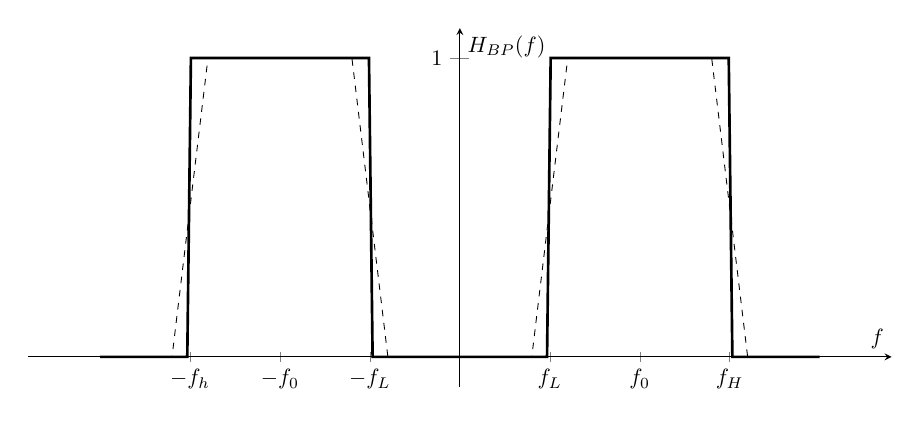
\begin{tikzpicture}[scale=.8]
	\begin{axis}[axis lines=middle,no markers,enlargelimits,xscale=2,xtick={-1.5,-1,-.5,0,.5,1,1.5},xticklabels={$-f_h$,$-f_0$,$-f_L$,$0$,$f_L$,$f_0$,$f_H$},ytick={0,1},xlabel=$f$,ylabel=$H_\text{BP}(f)$]
	\addplot [very thick,samples=100,domain=-2:0]  {abs(x+1)<.5?1:0};
	\addplot [very thick,samples=100,domain=0:2]  {abs(x-1)<.5?1:0};
	\addplot [dashed,samples=11,domain=-2:0]  {abs(x+1)<.5?1:0};
	\addplot [dashed,samples=11,domain=0:2]  {abs(x-1)<.5?1:0};
	\end{axis}
	\end{tikzpicture}
\end{figure}

Si definisce il \textsc{fattore di qualità} $Q=\frac{f_0}{B}$, che risulta tanto migliore quanto più è stretta la banda attorno alla frequenza $f_0$.
\begin{equation}H_\text{BP}(f)=\rect{\frac{f-f_0}{B}}+\rect{\frac{f+f_0}{B}}\end{equation}
\[h_\text{BP}(t)=B\sinc{B t}\e{\imath 2\pi f_0 t}+B\sinc{B t}\e{-\imath 2\pi f_0 t}=2 B\sinc{B t}\cos{2\pi f_0 t}\]

\begin{figure}[h!]
\centering\begin{tikzpicture}
\begin{axis}[axis lines=middle,no markers,enlargelimits,xscale=2,xtick={-9.424,-6.283,-3.141,0,3.141,6.283,9.424},ytick={0,2},xticklabels={$-\frac{3}{B}$,$-\frac{2}{B}$,$-\frac{1}{B}$,$0$,$\frac{1}{B}$,$\frac{2}{B}$,$\frac{3}{B}$},yticklabels={$0$,$2B$},ylabel={$h_\text{BP}(t)$}]
\addplot [thick,domain=-3.5*pi:3.5*pi,samples=300] { (2*sin(x)/x)*cos(8*x) };
\addplot [dashed,domain=-3.5*pi:3.5*pi,samples=100] { (2*sin(x)/x) };
\end{axis}\end{tikzpicture}\caption{Filtro passa banda ideale}
\end{figure}

\begin{esempio}
Esempio di filtro passa basso realizzato con circuito \textsc{RC}.
\begin{figure*}[h]
\centering\begin{circuitikz}
\draw (0,0)	to[open,v^>=${V_i(t)}$] (0,3)
	to[R, l=${R}$, *-] (3,3)
	to[C, l=${C}$,i>_=${i(t)}$] (3,0) to[short,-*] (0,0)
	(3,0) -- (4,0) to[open,v>=${V_u(t)}$, *-*] (4,3) -- (3,3)
	(1.5,1.5) node[scale=3]{$\circlearrowright$}
	(1.5,1.5) node{$i(t)$};
\end{circuitikz}\caption{Filtro passa basso realizzato con circuito RC}
\end{figure*}
La tensione sul condensatore $v_c$ pari alla tensione di uscita $v_u$
\[v_u(t)=\frac{q(t)}{C}\]
\[\deriv{v_u(t)}{t}=\frac{1}{C}i(t)\]
L'equazione differenziale che descrive l'andamento delle tensioni
\[v_i(t)=R i(t)+ v_u(t)=R C \deriv{v_u(t)}{t} + v_u(t)\]
Trasformata secondo Fourier
\[V_i(f)=R C \imath 2\pi f_o V_u(f) + V_u(f)\]
Funzione di trasferimento ingresso-uscita
\[H(f)=\frac{V_i(f)}{V_u(f)}=\frac{1}{1+\imath 2\pi f R C}\]
dove $f_T=\frac{1}{2\pi R C}$ rappresenta la frequenza di taglio.
\begin{figure}[h!]
\centering\begin{tikzpicture}[scale=.8]
\begin{axis}[axis lines=middle,no markers,enlargelimits,xscale=1.5,xtick={.159},xticklabels={$f_T$},ytick={0,1},xlabel=$f$,ylabel=$\abs{H(f)}$]
\addplot [very thick,samples=200,domain=-1:1]  {1/(sqrt(1+(2*pi*x)^2))};
\addplot [dashed] coordinates {(-.159,.707)(.159,.707)(.159,0)};
\end{axis}
\end{tikzpicture}
\caption{Modulo della funzione di trasferimento}
\end{figure}

La risposta in ampiezza espressa in decibel, come confronto tra potenze relative ad un riferimento
\[\abs{H(f)}_\text{dB}=10\Log\frac{\abs{H(f)}^2}{\abs{H(f_0)}^2}\]
si calcola sulla potenza del segnale, ovvero alla sua risposta in ampiezza al quadrato
\[\abs{H(f)}^2=\frac{1}{1+(2\pi f R C)^2}\]
calcolata rispetto al riferimento $f_0=0$ per cui $\abs{H(f_0)}^2=1$

Alla frequenza di taglio $f_T=\frac{1}{2\pi R C}$ si dimezza il modulo quadro ovvero si ha una attenuazione pari a 
\[\abs{H\left(f_T\right)}_\text{dB}=10\Log\frac{1}{2}=-3\text{dB}\]

\begin{figure}[h!]
	\centering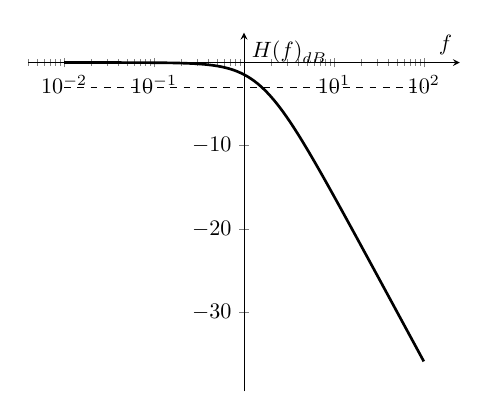
\begin{tikzpicture}[scale=.8]
	\begin{axis}[xmode=log,axis lines=middle,no markers,enlargelimits,xlabel=$f$,ylabel=$\abs{H(f)}_\text{dB}$]
	\addplot [very thick,samples=200,domain=.01:100]  {-10*log10( 1+(2*pi*x*.1)^2)};
	\addplot [dashed] coordinates{(.01,-3)(100,-3)};
	\end{axis}
	\end{tikzpicture}
	\caption{Modulo in decibel della funzione di trasferimento}
\end{figure}
\end{esempio}

\section{Autocorrelazione per segnali ad energia finita}
Si definisce per segnali ad energia finita la funzione \textsc{autocorrelazione}\index{segnale!autocorrelazione}, grandezza che indica quanto un segnale $x(t)$ sia simile ad una sua replica ritardata di un tempo $\tau$
\begin{equation}R_x(\tau)=\intinf{x(t)\conj{x}(t-\tau)}{t}=x(\tau)\ast \conj{x}(-\tau)\end{equation}
La trasformata di Fourier del prodotto di convoluzione \footnote{essendo $x(-t)\overset{\Fourier}{\to}X(-f)$ mentre $\conj{x}(t)\overset{\Fourier}{\to}\conj{X}(-f) \implies \conj{x}(-t)\overset{\Fourier}{\to}\conj{X}(f)$
}
\[x(\tau)\ast \conj{x}(-\tau)\overset{\Fourier}{\to}X(f)\conj{X}(f)\]

La funzione di autocorrelazione è anche l'antitrasformata di Fourier dello spettro di energia del segnale
\begin{equation}
R_x(\tau)=\intinf{\abs{X(f)}^2\e{\imath 2\pi f\tau}}{\tau}
\end{equation}

\textbf{Proprietà}
\begin{enumerate}
\item La funzione di autocorrelazione calcolata per $\tau=0$ coincide con l'energia del segnale
\[R_x(0)=\intinf{x^2(t)}{t}=E_x\]
\item La funzione di autocorrelazione è una funzione pari
\[R_x(\tau)=R_\conj{x}(-\tau)\]
\emph{Dim.} Facilmente dimostrabile in frequenza 
\[\begin{split}R_x(\tau)&=\intinf{\abs{X(f)}^2\e{\imath 2\pi f\tau}}{\tau}\\
R_x(-\tau)&=\intinf{\abs{X(f)}^2\e{-\imath 2\pi f\tau}}{\tau}\\
R_\conj{x}(-\tau)&=\intinf{\abs{X(f)}^2\e{\imath 2\pi f\tau}}{\tau}\end{split}\]
\item Il massimo della funzione di autocorrelazione si ha per $\tau=0$
\[\abs{R_x(\tau)}\leq R_x(0)\]
\emph{Dim.}
\[\begin{split}\abs{R_x(\tau)}^2=\abs{\intinf{x(t)x(t-\tau)}{t}}^2&\leq\intinf{\abs{x(t)}^2\abs{x(t-\tau)}^2}{t}\leq\\\leq&\intinf{\abs{x(t)}^2}{t}\cdot\intinf{\abs{x(t-\tau)}^2}{t}=R_x^2(0)\end{split}\]
\end{enumerate}

\section{Cross correlazione}
Si definisce la \keyword[segnali!cross-correlazione]{cross-correlazione} tra due segnali $x(t)$ e $y(t)$ la misura della somiglianza tra due segnali tra cui intercorre un ritardo di un tempo $\tau$
\begin{equation}R_{xy}(\tau)=\intinf{x(t)\conj{y}(t-\tau)}{t}=x(\tau)\ast \conj{y}(-\tau)\end{equation}
\begin{equation}R_{yx}(\tau)=\intinf{y(t)\conj{x}(t-\tau)}{t}=y(\tau)\ast \conj{x}(-\tau)\end{equation}
Si può dimostrare che \[R_{xy}(\tau)=R_\conj{yx}(-\tau)\] infatti se $R_{yx}(\tau)=y(\tau)\ast \conj{x}(-\tau)\implies R_\conj{yx}(\tau)=\conj{y}(\tau)\ast x(-\tau)\implies
R_\conj{yx}(-\tau)=\conj{y}(-\tau)\ast x(\tau)=R_{xy}$.

Due segnali si dicono \keyword[segnali!ortogonali]{ortogonali} se sono incorrelati qualunque sia il ritardo $\tau$ \[R_{xy}(\tau)=0\;\forall\tau\]

\section{Autocorrelazione per segnali a potenza finita}
Per i segnali a potenza finita si è definita la potenza (eq.\ref{eq:segnale_potenza}) come \[P_s=\lim\limits_{T\to+\infty}{\frac{1}{2T}\intd{-T}{T}{\abs{s(t)}^2}{t}}\]
Tale quantità si può definire anche nel dominio delle frequenze, come integrale della densità spettrale di potenza del segnale. Estraendo una limitazione del segnale $s_T(t)=s(t)\rect{\frac{t}{2T}}$ ristretta all'intervallo $[-T,T]$ essa ha sicuramente energia finita, pertanto se ne potrà esprimere la trasformata di Fourier, $s_T(t)\overset{\Fourier}{\to}S_T(f)$. Per il teorema di Parseval (eq.\ref{eq:parseval}) l'energia è distribuita nello spettro 
\[E_{s_T}=\intinf{\abs{s_T(t)}^2}{t}=\intinf{\abs{S_T(f)}^2}{f}\]

Si può quindi definire la potenza come limite dell'energia della limitazione $s_T(t)$ rapportata al periodo, al tendere dell'intervallo della limitazione all'infinito
\[P_s=\lim\limits_{T\to+\infty}{\frac{1}{2T}\intd{-T}{T}{\abs{s_T(t)}^2}{t}}=\lim\limits_{T\to+\infty}{\frac{1}{2T}\intinf{\abs{S_T(f)}^2}{f}}\]
Scambiando il limite con l'integrale si ha 
\[P_s=\intinf{\lim\limits_{T\to+\infty}\frac{1}{2T}\abs{S_T(f)}^2}{f}\]
la funzione integranda che si definisce \textsc{densità spettrale di potenza} o \textsc{spettro di potenza}
\begin{equation}
S_P(f)=\lim\limits_{T\to+\infty}{\frac{1}{2T}\abs{S_T(f)}^2}=\lim\limits_{T\to+\infty}{\frac{1}{2T}\;S_T(f)S_\conj{T}(f)}
\end{equation}
La densità spettrale di potenza gode di proprietà simili a quelle della densità spettrale di energia, ovvero è una funzione pari per segnali reali, è sempre non negativa e il suo integrale su tutte le frequenze restituisce la potenza complessiva del segnale.
Inoltre come per i segnali ad energia finita, il passaggio di un segnale a potenza finita attraverso un sistema lineare tempo invariante restituisce in uscita un segnale sempre a potenza finita, la cui densità spettrale risulterà $S_{P_y}(f)=S_{P_x}(f)\cdot\abs{H(f)}^2$

Antitrasformando la funzione densità spettrale di potenza si ottiene 
\[\Fourier^{-1}\left\lbrace{S_P(f)}\right\rbrace=\lim\limits_{T\to+\infty}{\frac{1}{2T}\;s_T(\tau)\ast s_\conj{T}(-\tau)}=\lim\limits_{T\to+\infty}{\frac{1}{2T}\intd{-T}{T}{s_T(t)s_\conj{T}(t-\tau)}{t}}\]
che è la funzione di \textsc{autocorrelazione} per segnali di potenza finita
\begin{equation}R_s(\tau)=\lim\limits_{T\to+\infty}{\frac{1}{2T}\intd{-T}{T}{s(t)\conj{s}(t-\tau)}{t}}\end{equation}

\chapter{Teoria della probabilità}

\section{Concetti di base}
Si definisce \textsc{spazio campione $\Omega$} l'insieme di tutti i possibili risultati di un esperimento o eventi. Un \textsc{evento} è un qualsiasi sotto insieme di possibili risultati di un esperimento, sottoinsieme di $\Omega$.

Dato $A$, un evento, si definisce il suo complemento $\bar{A}$, ovvero tutto lo spazio campione meno A, $\bar{A}=\Omega\setminus A$

$A\cup B$ (unione di A e B) è il sottoinsieme degli eventi che appartengono ad A o a B

$A\cup\bar{A}=\Omega$ l'unione di A e il complemento di A costituisce l'intero spazio campione

$A\cap B$ (intersezione di A e B) è il sottoinsieme degli eventi che appartengono sia ad A che a B

$A\cap\bar{A}=\emptyset$ l'intersezione tra eventi complementari è l'insieme vuoto.

\section{Spazio di probabilità}
Una definizione assiomatica di uno spazio di probabilità per \textsc{esperimenti aleatori} è caratterizzata da 
\begin{itemize}
\item uno spazio campione $\Omega$
\item un insieme $S$ degli eventi di interesse (non necessariamente $\Omega$)
\item una legge di probabilità $P(.)$ secondo Kolmogorov
\end{itemize}

\section{Legge di probabilità}
Una \textsc{legge di probabilità} secondo Kolmogorov mette in corrispondenza un evento $A\in S$ con un numero reale tale che
\begin{equation}P(A)\geq 0\end{equation}
\begin{equation}P(\Omega)=1\end{equation}
eventi mutualmente esclusivi \begin{equation}A\cap B=0\implies P(A\cup B)=P(A)+P(B)\end{equation}

\section{Modelli alternativi}
Modelli matematici alternativi di probabilità sono la definizione di Laplace secondo cui, per uno spazio campione finito e un esperimento simmetrico (esempio: lancio di un dado non truccato), la probabilità è calcolata come numero di eventi favorevoli fratto il numero di eventi possibili
\begin{equation}
P(A)=\frac{N_F(A)}{N_P(A)}
\end{equation}

Definizione di Van Mises o \emph{frequentista} per cui ripetendo $N$
volte un esperimento e contando il numero $N_A$ di volte in cui si verifica l'evento A, si ha che la \textsc{frequenza relativa} $\frac{N_A}{N}$ si approssima al valore della probabilità di A
\begin{equation}P(A)=\lim\limits_{N\to\infty}\frac{N_A}{N}
\end{equation}

La definizione frequentista rientra nella teoria assiomatica infatti
$P(A)=\frac{N_A}{N}\geq 0$, se $A=\Omega\implies N_A=N\implies P(A)=1$, inoltre 
e $A\cap B=\emptyset$ allora $N_{A\cup B}=N_A+N_B\implies P(A\cup B)= \lim\limits_{N\to\infty}\frac{N_{A\cup B}}{N}=\lim\limits_{N\to\infty}\frac{N_A+N_B}{N}=P(A)+P(B)$

\section{Teoremi}
A partire da tali assiomi si derivano i seguenti teoremi
\begin{equation}P(\bar{A})=1-P(A)\end{equation}

\begin{proof}[Dim.] $A\cup\bar{A}=\Omega\implies P(A\cup\bar{A})=1$

$A\cap\bar{A}=0\implies P(A\cup\bar{A})=P(A)+P(\bar{A})$
\end{proof}

\begin{equation}P(\emptyset)=0\end{equation}

\begin{proof}[Dim.] $\bar{\Omega}=\emptyset\implies P(\emptyset)=P(\bar{\Omega})=1-P(\Omega)=0$
\end{proof}

\begin{equation}0\leq P(A)\leq 1\end{equation}

\begin{proof}[Dim.] Per il primo assioma $P(A)\geq 0$ e $P(\bar{A})\geq 0$ ma è anche $P(A)=1-P(\bar{A})$
\end{proof}

\subsection{Teorema probabilità congiunte}
\begin{equation}P(A\cup B)=P(A)+P(B)-P(A\cap B)\end{equation}

\begin{proof}[Dim.] 
\[A\cup B=A\cup(B\cap\bar{A})\implies P(A\cup B)=P(A)+P(B\cap\bar{A})\]

\[B=B\cap(A\cup\bar{A})=(B\cap A)\cup(B\cap\bar{A})\implies P(B)=P(B\cap A)+P(B\cap\bar{A})\]
insieme $\implies P(A\cup B)=P(A)+P(B)-P(B\cap A)$
\end{proof}

\subsection{Teorema probabilità condizionata}
$P(A)$ è la probabilità che si verifichi l'evento A a priori.
$P(A|B)$ è la probabilità che si verifichi l'evento A dato che si sia verificato l'evento B, la prob. di A a posteriori:
\begin{equation}
P(A|B)=\frac{P(A\cap B)}{P(B)}
\end{equation}

Nel caso particolare che A e B siano \textsc{eventi indipendenti}, la probabilità che si verifichi A non è influenzata da B, pertanto \[P(A|B)=P(A)\qquad P(A\cap B)=P(A)P(B)\]

\subsection{Teorema di Bayes}
\begin{equation}
P(A|B)=\frac{P(B|A)P(A)}{P(B)}
\end{equation}
che si può verificare facilmente sostituendo alla prob. condizionata $P(B|A)=\frac{P(A\cap B)}{P(A)}$

\subsection{Teorema delle Probabilità Totali (Bayes)}
Data una partizione dello spazio campione $\bigcup_i B_i=\Omega, B_i\cap B_j=\emptyset \;\forall i\neq j$
\begin{equation}
P(A)=\sum_i P(A|B_i)P(B_i)
\end{equation}

\begin{proof}[Dim.]
Si dimostra facilmente notando che $A=\bigcup_i B_i \cap A=\bigcup_i (A\cap B_i) \implies P(A)=\sum_i P(A\cap B_i)=\sum_i P(A|B_i)P(B_i)$
\end{proof}

\section{Esperimento aleatorio composto}
Si considerano due esperimenti aleatori differenti caratterizzati ognuno dal proprio spazio campione. Si può considerare un esperimento composto in cui si osservano i due eventi $A_1\subseteq\Omega_1$ e $A_2\subseteq\Omega_2$, la coppia $A=A_1\times A_2$ nel nuovo spazio campione $\Omega_1\times\Omega_2$.

I due eventi possono essere indipendenti, in tal caso la probabilità dell'evento composto è pari al prodotto delle probabilità $P(A)=P(A_1)\cdot P(A_2)$.

Se i due esperimenti sono in qualche modo legati, si influenzano, sarà necessario invece valutare il grado di correlazione dei due eventi.

Le medesime considerazioni fatte per due esperimenti si possono fare per la composizione di $N$ qualsiasi esperimenti o prove ripetute ed indipendenti in un esperimento composto.

\subsection{Prove binarie di Bernoulli}
Esperimento composto da $n$ prove ripetute di esperimenti uguali tra loro e indipendenti, ciascuno con due soli possibili esiti $\omega_0$ e $\omega_1$ con probabilità $P(\omega_0)=p$ e $P(\omega_1)=1-p$.
Esempio classico il lancio di $n$ monete o il lancio ripetuto di una stessa moneta con risultato la sequenza di testa o croce.

Si definisce l'evento $A=\lbrace\omega_0$ si presenta $k$ volte in $n$ esperimenti$\rbrace$, $0\leq k\leq n$

La \textsc{formula binomiale di Bernoulli} esprime la probabilità dell'evento A:
\begin{equation}
P(A)=\binom{n}{k} p^k (1-p)^{n-k}
\end{equation}

Il coefficiente binomiale 
\begin{equation}\binom{n}{k}=\frac{n!}{k!(n-k)!}\end{equation}
tiene conto delle possibili \textsc{combinazioni} in cui $k$ elementi possono essere disposti in $n$ posizioni non distinguendoli per l'ordine. Si ottiene dal numero di \textsc{disposizioni} possibili di $k$ oggetti in $n$ posizioni distinguendo le posizioni $D_{n,k}=n\cdot(n-1)\dots(n-k+1)=\frac{n!}{(n-k)!}$ diviso il numero delle \textsc{permutazioni} $P_{n,k}=k!$ di $k$ oggetti in $n$ posizioni.

\section{Esempi esperimenti aleatori}
\begin{esempio}
Esperimento di estrazione di palline bianche e nere da 5 urne di 3 tipi:
\begin{itemize}
	\item $A_1$: 2 urne con 2 palline bianche 1 nera
	\item $A_2$: 1 urna con 10 palline nere
	\item $A_3$: 2 urne con 3 palline bianche 1 nera
\end{itemize}
Evento $E_1=\lbrace$ pallina estratta da urna a caso è bianca $\rbrace$
\[E_1=(A_1\cap W)\cup(A_2\cap W)\cup(A_3\cap W)\]
Per il teorema delle probabilità totali
\[P(E_1)=P(A_1\cap W)+P(A_2\cap W)+P(A_3\cap W)=\frac{4}{15}+0+\frac{3}{10}\]
dove per il teorema delle probabilità condizionate
\[\begin{split}P(A_1\cap W)&=P(W|A_1) P(A_1)=\frac{2}{3}\cdot\frac{2}{5}=\frac{4}{15}\\
P(A_2\cap W)&=P(W|A_2) P(A_2)=0\cdot\frac{1}{5}=0\\
P(A_3\cap W)&=P(W|A_3) P(A_3)=\frac{3}{4}\cdot\frac{2}{5}=\frac{3}{10}\end{split}\]

Evento $E_2=\lbrace$ pallina estratta a caso sia bianca da urna di tipo 3 $\rbrace$
\[E_2=(A_1\cap W)\cup(A_2\cap W)\cup(A_3\cap W)\]

Per il teorema di Bayes la probabilità condizionata è
\[P(E_2)=P(A_3|W)=\frac{P(W|A_3)P(A_3)}{P(W)}=\frac{\frac{3}{4}\cdot\frac{2}{5}}{\frac{17}{30}}=\frac{3}{4}\cdot\frac{2}{5}\cdot\frac{30}{17}=\frac{9}{17}\cong 0,529\]
\end{esempio}

\begin{esempio}
Esperimento aleatorio composto
\begin{itemize}
\item 1 scatola con 2000 articoli di cui 5\% grandi
\item 1 scatola con 500 articoli di cui 40\% grandi
\item 1 scatola con 1000 articoli di cui 10\% grandi
\item 1 scatola con 1000 articoli di cui 10\% grandi
\end{itemize} 
Si scelga una scatola a caso e si estragga un articolo a caso e si valuti la probabilità $P(G)$ che sia estratto un articolo grande.

Per il teorema delle probabilità totali ho
\[P(G)=\sum_{i=1}^{4}P(G|S_i)P(S_i)\]

$P(S_i)=\frac{1}{4}$, $P(G|S_1)=0.05$, $P(G|S_2)=0.4$, $P(G|S_3)=0.1$, $P(G|S_4)=0.1$

\[P(G)=\frac{1}{4}(0.05+0.4+0.1+0.1)=\frac{1}{4}\cdot 0.65=0.1625\]
Nel caso sia estratto un articolo grande, quale è la probabilità che sia dalla scatola 3?

Per il teorema di Bayes
\[P(S_3|G)=\frac{P(G|S_3)P(S_3)}{P(G)}=0.1\cdot\frac{1}{4}\cdot\frac{1}{0.1625}\cong 0.154\]
\end{esempio}

\begin{esempio}
Esperimento aleatorio composto

Ho 6 scatole di 3 tipi diversi ognuna con 12 palline alcune bianche alcune nere 
\begin{itemize}
	\item $A_1$ 1 scatola con 7 palline bianche 5 nere
	\item $A_2$ 2 scatola con 5 palline bianche 7 nere
	\item $A_3$ 3 scatola con 4 palline bianche 8 nere
\end{itemize}
Ad ogni estrazione la pallina viene rimessa nella scatola.

Qual è la probabilità dell'evento $E=\lbrace 2B+1N \rbrace$ ?

Si può scomporre l'evento in eventi disgiunti ed applicare il teorema delle probabilità totali
\[P(E)=\sum_{i=1}^{3}P(E|A_i)P(A_i)\]
dove data la ripartizione delle scatole $P(A_1)=\frac{1}{6}, P(A_2)=\frac{2}{6}=\frac{1}{3}, P(A_3)=\frac{3}{6}=\frac{1}{2}$  
Le probabilità condizionate si calcolano come prove ripetute di Bernoulli binarie indipendenti sull'evento E:
\[\begin{split}
P(E|A_1)&=\binom{3}{2}P(B|A_1)^2 P(N|A_1)=3\left(\frac{7}{12}\right)^2\frac{5}{12}=\frac{5}{4}\left(\frac{7}{12}\right)^2\\
P(E|A_2)&=\binom{3}{2}P(B|A_2)^2 P(N|A_2)=3\left(\frac{5}{12}\right)^2\frac{7}{12}=\frac{7}{4}\left(\frac{5}{12}\right)^2\\
P(E|A_3)&=\binom{3}{2}P(B|A_3)^2 P(N|A_3)=3\left(\frac{4}{12}\right)^2\frac{8}{12}=\frac{2}{9}
\end{split}\]

\[\begin{split}P(E)&=P(E|A_1)P(A_1)+P(E|A_2)P(A_2)+P(E|A_3)P(A_3)=\\
&=\frac{1}{6}\cdot\frac{5}{4}\left(\frac{7}{12}\right)^2+\frac{1}{3}\cdot\frac{7}{4}\left(\frac{5}{12}\right)^2+\frac{1}{2}\cdot\frac{2}{9}\cong 0.28\end{split}\]

Qual è la probabilità che si verifichi l'evento $E=\lbrace 2B+1N\rbrace$ da scatole del tipo $A_3$?
Per il teorema di Bayes
\[P(A_3|E)=\frac{P(E|A_3)P(A_3)}{P(E)}=\frac{2}{9}\cdot\frac{1}{2}\cdot\frac{1}{0.28}\cong 0,39\]
\end{esempio}

\chapter{Variabili aleatorie continue e discrete}
\section{Variabili aleatorie}
Si consideri un esperimento aleatorio avente spazio campione $\Omega$, classe degli eventi $S$, legge di probabilità $P(\cdot)$, si definisce una corrispondenza $X(\omega_i)$ che associ a ciascun evento $\omega_i\in\Omega$ un unico numero reale $a\in\R$.

Se l'insieme dei risultati di un esperimento aleatorio per i quali è verificata la disuguaglianza $X(\omega)\leq a$ è un evento, $\forall a\in\R$, si dice che $X$ è una \keyword[variabile aleatoria]{variabile aleatoria}.

Tale definizione di variabile aleatoria modella un esperimento che ha un risultato numerico non prevedibile a priori derivato da una operazione di misura. Ripetendo un esperimento si otterrà un insieme di misure che rappresenta la variabile aleatoria.\\

\section{Funzione distribuzione di probabilità}
Si vuole ora stabilire come trasferire la legge di probabilità sugli eventi alle variabili aleatorie che vi associa numeri sull'asse reale.

Si definisce \keyword[variabile aleatoria!funzione distribuzione di probabilità]{funzione distribuzione di probabilità} di una variabile aleatoria $X$ la funzione che associa per un fissato valore reale $x$ il valore della probabilità dell'evento $\lbrace X\leq x\rbrace$:
\begin{equation}
F_X(s)=P(X\leq x)
\end{equation}\label{eq:funz_dist_prob}

\textbf{Proprietà funzione distribuzione di probabilità}
\begin{enumerate}
\item $0\leq F_X(x)\leq 1$
\item $\lim\limits_{x\to+\infty}F_X(x)=1$
\item $\lim\limits_{x\to-\infty}F_X(x)=0$
\item $F_X$ è monotona non decrescente: \[x_1<x_2\implies F_X(x_1)\leq F_X(x_2)\] 
\item $F_X$ è continua a destra: \[\lim\limits_{h\to 0^+}{F_X(x+h)}=F_X(x)\]
\item se $F_X$ presenta discontinuità di prima specie in $\bar{x}$ la probabilità dell'evento $X=\bar{x}$ è pari alla differenza tra limite destro e sinistro \[P(X=\bar{x})=\lim\limits_{h\to 0^+}{F_X(x+h)} - \lim\limits_{h\to 0^-}{F_X(x+h)}\]
\item la probabilità dell'evento $a < X \leq b$:
\[P(a<X\leq b)=F_X(b)-F_X(a)\]
\end{enumerate}

Le variabili aleatorie possono essere \emph{continue}, \emph{discrete} o \emph{miste} in base alla continuità della funzione distribuzione di probabilità $F_X(x)$.

Una variabile aleatoria discreta ha la funzione di distribuzione di probabilità continua a tratti: $F_X(x)=\sum_k P(X=x_k)\step{(x-x_k)}$, la probabilità è concentrata in “masse” di probabilità $p_k=P(X=x_k)$ in corrispondenza dei punti di discontinuità $x_k$.

Una variabile aleatoria continua ha la funzione distribuzione di probabilità continua, ovvero la probabilità che la variabile aleatoria assuma un particolare valore $P(X=\bar{x})$ è un infinitesimo. 

\section{Funzione densità di probabilità}
Si può dare una definizione alternativa di variabile aleatoria legata alla \keyword[variabile aleatoria!funzione densità di probabilità]{funzione densità di probabilità}
\begin{equation}\label{eq:funz_dens_prob}
f_X(x)=\deriv{F_X(x)}{x}
\end{equation}
dove la funzione di distribuzione di probabilità è
\begin{equation}F_X(x)=\intd{-\infty}{x}{f_X(\alpha)}{\alpha}\end{equation}

\textbf{Proprietà funzione densità di probabilità}
\begin{enumerate}
\item $f_X(x)\geq 0$
\item $P(a<X\leq b)=F_X(b)-F_X(a)=\intd{a}{b}{f_X(x)}{x}$
\item $\lim\limits_{x\to+\infty}f_X(x)=0\qquad\lim\limits_{x\to-\infty}f_X(x)=0$
\item $\intinf{f_X(x)}{x}=1$
\item $P(x<X\leq x+\Delta x)=\intd{x}{x+\Delta x}{f_X(\alpha)}{\alpha}\cong f_X(x)\Delta x$
\end{enumerate}

Per variabile aleatoria discreta la densità di probabilità è concentrata in impulsi
\begin{equation}f_X(x)=\sum_k P(X=x_k) \delta(x-x_k)\end{equation}

Se la variabile aleatoria è continua la densità di probabilità è distribuita con continuità.
Se la variabile aleatoria è mista la densità di probabilità è distribuita con continuità e in impulsi in cui sono concentrate masse di probabilità.

\section{Operazioni su variabili aleatorie}
Data una variabile aleatoria $X$ è possibile ottenere una nuova variabile aleatoria $Y=g(X)$ con funzione di distribuzione di probabilità
\begin{equation}F_Y(y)=P(Y\leq y)=P(g(X)\leq y)\end{equation}
Nel dominio $D_Y=\left\lbrace x\ni' g(x)\leq y\right\rbrace$ dei valori di $x$ per i quali $g(x)\leq y$ è possibile calcolare la funzione distribuzione di probabilità $F_Y(y)=\int_{D_Y}{f_X(x)\diff x}$ e la funzione densità di probabilità $f_Y(y)=\deriv{F_Y(y)}{y}$

Nel caso particolare di funzione $g(\cdot)$ sia monotona strettamente crescente o strettamente decrescente è possibile definire la sua inversa $g^{-1}(\cdot)$ per cui nel primo caso
\[F_Y(y)=P(Y\leq y)=P(g(X)\leq y)=P(X\leq g^{-1}(y))=F_X(g^{-1}(y))\implies\]
\begin{equation}
f_Y(y)=f_X(g^{-1}(y))\cdot\deriv{g^{-1}(y)}{y}=\restrict{\frac{f_X(x)}{g'(x)}}{x=g^{-1}(y)}
\end{equation}
Nel caso di funzione $g(\cdot)$ strettamente decrescente $g(x)\leq y\iff x>g^{-1}(y)$
\[F_Y(y)=P(Y\leq y)=P(g(X)\leq y)=P(X>g^{-1}(y))=1-F_X(g^{-1}(y))\implies\]
\begin{equation}
f_Y(y)=f_X(g^{-1}(y))\cdot-\deriv{g^{-1}(y)}{y}=\restrict{-\frac{f_X(x)}{g'(x)}}{x=g^{-1}(y)}
\end{equation}
In generale nel dominio di definizione $D_Y=\left\lbrace x\ni' g(x)\leq y\right\rbrace$
\begin{equation}
F_Y(y)=\int\limits_{D_Y}{\frac{f_X(x)}{\abs{g'(x)}}\diff x}
\end{equation}
ponendo attenzione al caso $g'(x)=0$ da trattare con attenzione, anche $f_X(x)$ può annullarsi, ovvero essere costanti sia $F_X(x)$ che $g(x)$.

\section{Indici statistici di variabile aleatoria}
Il massimo di informazione che si può trarre da un esperimento aleatorio è la funzione densità di probabilità che caratterizza la variabile aleatoria.
Quando non si conosce questa funzione è comunque possibile determinare dei parametri statistici che permettono di descriverne alcune proprietà.\\

Il più importante parametro statistico è il \keyword[valor medio]{valor medio} $\mu_X$ di v.a. continua $X$:
\begin{equation}\label{eq:v_a_media}
\mu_X=\intinf{x f_X(x)}{x}
\end{equation}
Per variabile aleatoria discreta si ha $f_X(x)=\sum_k p_k\delta(x-x_k)$, il valor medio
\begin{equation}\label{eq:v_a_discreta_media}
\mu_X=\intinf{x f_X(x)}{x}=\sum_k p_k \intinf{x \delta(x-x_k)}{x}=\sum_k x_k p_k
\end{equation}

\`{E} possibile calcolare il valor medio $\mu_Y$ di funzione trasformata di v.a. $Y=g(X)$ introducendo l'\keyword{operatore!aspettazione}{operatore aspettazione}
\begin{equation}
\E{g(X)}=\intinf{g(x)f_X(x)}{x}
\end{equation}
che nel caso della media assume la semplice relazione $\mu_X=\E{X}$.

L'operatore valor medio gode della proprietà di linearità, data dall'integrale, per cui 
\begin{equation}\E{a\cdot g(X)+b\cdot h(X)}=a \E{g(X)}+b \E{h(X)}\end{equation}

Per variabile aleatoria $Y=g(X)$ ottenuta da trasformazione si ha la notevole semplificazione di non dover calcolare la funzione densità di probabilità $f_Y$ nota $f_X$.
Per il \textsc{teorema del valor medio} si può calcolare direttamente il valor medio
\begin{equation}\label{eq:teo_valor_medio}
\mu_Y=\E{Y}=\E{g(X)}=\intinf{g(x) f_X(x)}{x}
\end{equation}

Due variabili aleatorie possono avere lo stesso valor medio pur avendo distribuzioni di probabilità differenti. Si quantifica questo indice statistico introducendo il parametro \keyword[varianza]{varianza} di variabile aleatoria continua definita come
\begin{equation}\label{eq:v_a_varianza}
\sigma^2_X=\E{(X-\mu_X)^2}=\intinf{(x-\mu_X)^2 f_X(x)}{x}
\end{equation}

La varianza di variabile aleatoria discreta
\begin{equation}\label{eq:v_a_varianza_discreta}
\sigma^2_X=\E{(X-\mu_X)^2}=\sum_k {(x-\mu_X)^2 p_k}
\end{equation}

Una misura di quanto sia dispersa la probabilità attorno alla media è data dalla \textsc{deviazione standard} $\sigma_X$, la radice quadrata della varianza.\\

Si definisce \textsc{momento di ordine $k$} l'aspettazione della potenza k di v.a.
\begin{equation}
\E{X^k}=\intinf{x^k f_X(x)}{x}
\end{equation}

Nel caso particolare $k=2$ si ha l'indice \textsc{valore quadratico medio} o \textsc{potenza} statistica di v.a.
\begin{equation}\label{eq:v_a_valore_quad_medio}
m^2_X=\E{X^2}=\intinf{x^2 f_X(x)}{x}\end{equation}
\begin{nota}Il valor quadratico medio è associato alla potenza del segnale, un parametro importante per il dimensionamento di un sistema di telecomunicazioni.\end{nota}
Varianza e potenza sono legate dalla relazione
\begin{equation}\begin{split}
\sigma^2_X&=\E{(X-\mu_X)^2}=\E{X^2-2X\mu_X+\mu^2_X}=\\
&=\E{X^2}-2\E{X}\mu_X+\mu^2_X=m^2_X-2\mu^2_X+\mu^2_X=\\&=m^2_X-\mu^2_X\end{split}\end{equation}
quindi $\E{X^2}=m^2_X=\sigma^2_X+\mu^2_X$

\section{Funzione generatrice dei momenti}
Per il calcolo degli indici statistici di variabili aleatorie più complesse ci si avvale della \textsc{funzione generatrice dei momenti}, definita come aspettazione della variabile aleatoria trasformata $\e{t X}$:
\begin{equation}\begin{split}
G_X(t)&=\E{\e{t X}}=\intinf{\e{t x}f_X(x)}{x}=\\
\intertext{sviluppando in serie di Taylor l'esponenziale}
&=\E{1+x t+\frac{(x t)^2}{2}+\frac{(x t)^3}{3!}+\dots+\frac{(x t)^k}{k!}}=\sum_{k=0}^{+\infty}{\frac{\E{x^k}}{k!}t^k}
\end{split}\end{equation}

Si definiscono i momenti di ordine $k$ come derivata della funzione generatrice calcolata in $t=0$.

\begin{description}
\item[Momento del primo ordine (valor medio)]
\begin{equation}
\restrict{\deriv{G_X(t)}{t}}{t=0}=\E{X}=\mu_X
\end{equation}
\item[Momento del secondo ordine (potenza)]
\begin{equation}
\restrict{\deriv[2]{G_X(t)}{t}}{t=0}=\E{X^2}
\end{equation}
\item[Momendo di ordine $k$]
\begin{equation}
\restrict{\deriv[k]{G_X(t)}{t}}{t=0}=\E{X^k}
\end{equation}
\end{description}

\section{Variabile aleatoria uniforme}
La \textsc{variabile aleatoria uniforme} presenta una densità di probabilità costante nell'intervallo $[a,b]$ e zero altrove. Dovendo sottendere un'area unitaria si ha un rettangolo di altezza costante $1/(b-a)$, base $(b-a)$ centrato in $(b+a)/2$
\begin{equation}f_X(x)=\begin{cases}0&x\leq a\\ \frac{1}{b-a}&a<x\leq b\\0&x>b\end{cases}\quad f_X(x)=\frac{1}{b-a}\rect{\frac{x-\frac{b+a}{2}}{b-a}}\end{equation}
La funzione distribuzione essendone l'integrale ha la definizione di una rampa
\begin{equation}F_X(x)=\begin{cases}
0&x\leq a\\ \frac{x-a}{b-a}&a<x\leq b\\1&x>b
\end{cases}\end{equation}
\begin{figure}[h!]
	\centering
	\subfloat[][$f_X(x)$]
	{\begin{tikzpicture}[scale=.7]
		\begin{axis}[axis lines=middle,no markers,enlargelimits,xscale=1.2,xtick={1,2,3},xticklabels={$a$,$\frac{b+a}{2}$,$b$},ytick={2},yticklabels={$\frac{1}{b-a}$},xlabel={$x$}]
		\addplot [very thick] coordinates{(-1,0)(1,0)(1,2)(3,2)(3,0)(4,0)};
		\end{axis}\end{tikzpicture}}\qquad
	\subfloat[][$F_X(x)$] {
		\begin{tikzpicture}[scale=.7]
		\begin{axis}[axis lines=middle,no markers,enlargelimits,xscale=1.2,xtick={1,2,3},xticklabels={$a$,$\frac{b+a}{2}$,$b$},ytick={1},xlabel={$x$}]
		\addplot [very thick] coordinates{(-1,0)(1,0)(3,1)(4,1)};
		\end{axis}\end{tikzpicture}	
	}
	\caption{Variabile aleatoria uniforme}
\end{figure}

\begin{description}
\item[Valor medio]\[\mu_X=\intd{a}{b}{\frac{1}{b-a}x}{x}=\frac{1}{b-a}\bound{a}{b}{\frac{x^2}{2}}=\frac{b+a}{2}\]
\item[Valor quadratico medio] \[\E{X^2}=\intd{a}{b}{\frac{1}{b-a}x^2}{x}=\frac{1}{b-a}\bound{a}{b}{\frac{x^3}{3}}=\frac{1}{3}\frac{b^3-a^3}{b-a}=\frac{b^2+a b+a^2}{3}\]
\item[Varianza]\[\sigma^2_X=\E{X^2}-\mu^2_X=\frac{b^2+a b+a^2}{3}-\left(\frac{b+a}{2}\right)^2=\frac{(b-a)^2}{12}\]
\item[Deviazione standard]\[\sigma_X=\frac{b-a}{2\sqrt{3}}\]
\item[Deviazione standard normalizzata]\[\frac{\sigma_X}{\mu_X}=\frac{\frac{b-a}{2\sqrt{3}}}{\frac{b+a}{2}}=\frac{b-a}{b+a}\frac{1}{\sqrt{3}}\]
\end{description}

\section{Variabile aleatoria esponenziale}
La \textsc{variabile aleatoria continua esponenziale} unilatera con parametro $\lambda>0$ ha una funzione densità di probabilità che parte con una discontinuità in $x=0$ e decresce esponenzialmente a zero. Utile a modellare i tempi di intercorrenza tra richieste di un servizio, problemi di affidabilità e calcolo del rischio. La coda indica eventi rari trascurabili, caratteristica che aiuta a dimensionare i sistemi.
\begin{equation}
f_X(x)=\lambda\e{-\lambda x}\step(x)
\end{equation}
\begin{equation}
F_X(x)=\intd{-\infty}{x}{f_X(\alpha)}{\alpha}=\intd{-\infty}{x}{\lambda\e{-\lambda \alpha}}{\alpha}=1-\e{-\lambda x}
\end{equation}
\begin{figure}[h!]
	\centering
	\subfloat[][$f_X(x)=\lambda\e{-\lambda x}$]
	{\begin{tikzpicture}[scale=.67]
		\begin{axis}[axis lines=middle,no markers,enlargelimits,xtick={0},ytick={0,2},yticklabels={0,$\lambda$},ylabel={$f_X(x)$}]
		\addplot [very thick,domain=-1:3,samples=200] {x>0?2*exp(-2*x):0};
		\end{axis}\end{tikzpicture}} \qquad
	\subfloat[][$F_X(x)=1-\e{-\lambda x}$] {
		\begin{tikzpicture}[scale=.7]
		\begin{axis}[axis lines=middle,no markers,enlargelimits,xtick={0},ytick={0,1},ylabel={$F_X(x)$}]
		\addplot [very thick,domain=-1:3,samples=100] {x>0?1-exp(-2*x):0};
		\end{axis}\end{tikzpicture}	
	}
	\caption{Variabile aleatoria esponenziale}
\end{figure}

\begin{description}
\item[Valor medio]
\begin{equation}\begin{split}\mu_X&=\intinf{x f_X(x)}{x}=\intd{0}{+\infty}{x \lambda\e{-\lambda x}}{x}=\\
\intertext{integrando per parti $\int{u \diff v}=u v-\int{v\diff u}, u=\lambda x$, $\diff u=\lambda\diff x$, $\diff v=\e{-\lambda x}\diff x$, $v=-\frac{1}{\lambda}\e{-\lambda x}$}
&=\bound{0}{+\infty}{-x\e{-\lambda x}}+\intd{0}{+\infty}{\e{-\lambda x}}{x}=\frac{1}{\lambda} 	\qquad\text{essendo} \int\lambda\e{-\lambda x}\diff x=1\end{split}\end{equation}
\item[Potenza]
\begin{equation}\begin{split}
\E{X^2}&=\intinf{x^2 f_X(x)}{x}=\intd{0}{+\infty}{\lambda x^2\e{-\lambda x}}{x}=\\
\intertext{integrando per parti $u=x^2$, $\diff u=2x\diff x$, $\diff v=\lambda\e{-\lambda x}$, $v=-\e{-\lambda x}$}
&=\bound{0}{+\infty}{-x^2\e{-\lambda x}}+\frac{1}{\lambda}\intd{0}{+\infty}{2x \lambda\e{-\lambda x}}{x}=\frac{2}{\lambda^2}
\end{split}\end{equation}
\item[Varianza]
\[\sigma^2_X=\E{X^2}-\mu^2_X=\frac{2}{\lambda^2}-\frac{1}{\lambda^2}=\frac{1}{\lambda^2}\]
\item[Deviazione standard]
\[\sigma_X=\frac{1}{\lambda}=\mu_X\]
\item[Deviazione standard normalizzata dalla media] \[\frac{\sigma_X}{\mu_X}=1\]
\end{description}

\section{Variabile aleatoria discreta di Poisson}
La \textsc{variabile aleatoria discreta di Poisson} modella le richieste di servizio o il conteggio per arrivi indipendenti in un intervallo di tempo $T$ e con un parametro di intensità $\Lambda>0$ in istanti di tempo discreti (valori interi non negativi). La funzione densità di probabilità (di massa) $f_X(x)=\sum_k p_k \delta(x-k)$ ha espressione
\begin{equation}
f_X(x)=\sum_{k=0}^{+\infty}{\frac{(\Lambda T)^k}{k!}\e{-\Lambda T}\delta(x-k)}
\end{equation}
La funzione distribuzione di probabilità (di massa) $F_X(x)=\sum_k p_k \step(x-k)$ ha espressione
\begin{equation}
F_X(x)=\sum_{k=0}^{+\infty}{\frac{(\Lambda T)^k}{k!}\e{-\Lambda T}\step(x-k)}
\end{equation}
con massa di probabilità $p_k=\frac{(\Lambda T)^k}{k!}\e{-\Lambda T}$.

Calcolo indici statistici:
\begin{description}
\item[Valor medio]
\begin{equation}\begin{split}\mu_X&=\sum_{k=0}^{+\infty}{k p_k}=\sum_{k=0}^{+\infty}{k \frac{(\Lambda T)^k}{k!}\e{-\Lambda T}}=\sum_{k=1}^{+\infty}{\frac{(\Lambda T)^k}{(k-1)!}\e{-\Lambda T}}=\\
&=\Lambda T \e{-\Lambda T} \sum_{k=1}^{+\infty}{\frac{(\Lambda T)^{k-1}}{(k-1)!}}=\Lambda T \e{-\Lambda T}\sum_{z=0}^{+\infty}{\frac{(\Lambda T)^z}{z!}}=\Lambda T \e{-\Lambda T}\e{\Lambda T}=\\
&=\Lambda T
\end{split}\end{equation}
\item[Potenza]
\begin{equation}\begin{split}
\E{X^2}&=\sum_{k=0}^{+\infty}{k^2 p_k}=\sum_{k=0}^{+\infty}{k^2 \frac{(\Lambda T)^k}{k!}\e{-\Lambda T}}=\e{-\Lambda T}\sum_{k=0}^{+\infty}{k\frac{(\Lambda T)^k}{(k-1)!}}=\\
&=\e{-\Lambda T}\sum_{k=1}^{+\infty}{k\frac{(\Lambda T)^{z-1}}{(k-1)!}\Lambda T}=
\e{-\Lambda T}\sum_{k=1}^{+\infty}{(k-1+1)\frac{\Lambda T(\Lambda T)^{z-1}}{(k-1)!}}=\\
&=\e{-\Lambda T}\left[\sum_{k=1}^{+\infty}{(k-1)\frac{\Lambda T(\Lambda T)^{z-1}}{(k-1)!}} + \sum_{k=1}^{+\infty}{\frac{\Lambda T(\Lambda T)^{z-1}}{(k-1)!}}\right]=\\
&=\e{-\Lambda T}\left[\sum_{z=0}^{+\infty}{z\frac{\Lambda T(\Lambda T)^z}{z!}} + \Lambda T\e{\Lambda T}\right]=\\
&=\e{-\Lambda T}\left[\sum_{z=1}^{+\infty}{\frac{\Lambda T(\Lambda T)^{z-1}}{(z-1)!}} + \Lambda T\e{\Lambda T}\right]=\\
&=\e{-\Lambda T}\left[(\Lambda T)^2 \e{\Lambda T} + \Lambda T\e{\Lambda T}\right]=\\
&=(\Lambda T)^2 + \Lambda T
\end{split}\end{equation}
\end{description}

Gli stessi indici possono essere calcolati più agevolmente con la funzione generatrice dei momenti:
\begin{equation}G_X(t)=\sum_{k=0}^{+\infty}{\e{t x}p_k\delta(x-k)}=\sum_{k=0}^{+\infty}{\e{t k}\frac{(\Lambda T)^k}{k!}\e{-\Lambda T}}=\sum_{k=0}^{+\infty}{\frac{(\e{t}\Lambda T)^k}{k!}\e{-\Lambda T}}=\e{-\Lambda T}\e{\Lambda T\e{t}}\end{equation}

\begin{description}
\item[Valor medio (momento primo ordine)]
\begin{equation}\begin{split}\mu_X&=\restrict{\deriv{G_X(t)}{t}}{t=0}=\restrict{\deriv{\e{-\Lambda T}\e{\Lambda T\e{t}}}{t}}{t=0}=\restrict{\e{-\Lambda T}{\Lambda T}\e{t}\e{\Lambda T\e{t}}}{t=0}=\Lambda T \e{-\Lambda T}\e{\Lambda T}=\\&=\Lambda T\end{split}\end{equation}

\item[Potenza (momento secondo ordine)]
\begin{equation}\begin{split}\E{X^2}&=\restrict{\deriv[2]{G_X(t)}{t}}{t=0}=
\restrict{\deriv{\e{-\Lambda T}{\Lambda T}\e{t}\e{\e{t}\Lambda T}}{t}}{t=0}=
\restrict{\e{-\Lambda T}{\Lambda T}\deriv{\e{t}\e{\e{t}\Lambda T}}{t}}{t=0}=\\
&={\e{-\Lambda T}\Lambda T}\restrict{\left[\e{t}\e{\e{t}\Lambda T}+\e{t}\e{\e{t}\Lambda T}{\e{t}\Lambda T}\right]}{t=0}=\\
&={\e{-\Lambda T}\Lambda T}[\e{\Lambda T}+\e{\Lambda T}{\Lambda T}]=\\&=(\Lambda T)^2+\Lambda T
\end{split}\end{equation}
\end{description}

\section{Variabile aleatoria binomiale o di Bernoulli}
Variabile aleatoria discreta applicata ad esperimenti ripetuti di Bernoulli, indipendenti tra loro, che possono dare due soli possibili risultati, successo con probabilità $p$ e insuccesso con probabilità $1-p$. La variabile binomiale conta il numero di successi.
La funzione densità di probabilità (di massa) $f_X(x)=\sum_k p_k \impulse(x-k)$ e la funzione distribuzione di probabilità (di massa) $F_X(x)=\sum_k p_k \step(x-k)$ hanno massa di probabilità data dalla formula binomiale di Bernoulli:
\begin{equation}
P(X=k)=\binom{n}{k} p^k (1-p)^{n-k}\quad k=0,\dots,n
\end{equation}
Funzione generatrice dei momenti
\begin{equation}\begin{split}G_X(t)=\E{\e{t X}}&=\sum_{k=0}^{n}{\e{t k}\binom{n}{k}p^k(1-p)^{n-k}}=\\&=\sum_{k=0}^{n}{\binom{n}{k}(p\e{t})^k(1-p)^{n-k}}=\\
&=(p\e{t}+1-p)^n\end{split}\end{equation}
Calcolo degli indici statistici utilizzando la funzione generatrice dei momenti.\\

\begin{description}
\item[Valor medio]
\begin{equation}\begin{split}
\mu_X&=\restrict{\deriv{G_X(t)}{t}}{t=0}=\restrict{n(p\e{t}+1-p)^{n-1}p\e{t}}{t=0}=n p\end{split}\end{equation}
\item[Potenza]
\begin{equation}\begin{split}
\E{X^2}&=\restrict{\deriv[2]{G_X(t)}{t}}{t=0}=\restrict{\deriv{np\e{t}(p\e{t}+1-p)^{n-1}}{t}}{t=0}=\\
&=\restrict{np\e{t}(p\e{t}+1-p)^{n-1}+np\e{t}(n-1)(p\e{t}+1-p)^{n-2}p\e{t}}{t=0}=\\
&=np+np^2(n-1)=\\
&=np[p(n-1)+1]
\end{split}\end{equation}
\item[Varianza]
\begin{equation}\begin{split}
\sigma^2_X&=\E{X^2}-\Esp^2[X]=np[p(n-1)+1]-n^2p^2=\\
&=np+n^2p^2-np^2-n^2p^2=\\
&=np(1-p)\end{split}
\end{equation}
\end{description}

\section{Variabile aleatoria geometrica}
In esperimenti indipendenti e ripetuti di Bernoulli si vuole calcolare la probabilità di osservare $k$ successi prima di ottenere il primo insuccesso. La variabile aleatoria \textsc{geometrica} ha pertanto massa di probabilità
\begin{equation}
P(X=k)=p^k(1-p)\quad k=0,\dots,\infty
\end{equation}
La funzione generatrice dei momenti
\[\begin{split}G_X(t)=\E{\e{t X}}&=\sum_{k=0}^{\infty}{\e{t k}p^k(1-p)}=(1-p)\sum_{k=0}^{\infty}{(p\e{t})^k}=\\
&=\frac{1-p}{1-p\e{t}}=(1-p)(1-p\e{t})^{-1}\end{split}\]
dove la serie geometrica $\sum_{k=0}^{\infty}{(p\e{t})^k}$ converge in un intorno di $t=0$ dove calcoliamo i momenti.

\begin{description}
\item[Valor medio]
\begin{equation}
\mu_X=\restrict{\deriv{G_X(t)}{t}}{t=0}=\restrict{(1-p)(-1)(1-p\e{t})^{-2}(-p\e{t})}{t=0}=\frac{p}{1-p}
\end{equation}
\item[Potenza]
\begin{equation}
\begin{split}
\E{X^2}&=\restrict{\deriv[2]{G_X(t)}{t}}{t=0}=\restrict{\deriv{p(1-p)\e{t}(1-p\e{t})^{-2}}{t}}{t=0}=\\
&=p(1-p)\restrict{[\e{t}(1-p\e{t})^{-2}+\e{t}2(1-p\e{t})^{-3}p]}{t=0}=\\
&=p(1-p)[(1-p)^{-2}+2p(1-p)^{-3}]=\\
&=p(1-p)\frac{(1-p)+2p}{(1-p)^3}=\\
&=\frac{p(1+p)}{(1-p)^2}
\end{split}
\end{equation}
\item[Varianza]
\begin{equation}
\sigma^2_X=\E{X^2}-\Esp^2[X]=\frac{p(1+p)}{(1-p)^2}-\frac{p^2}{(1-p)^2}=\frac{p}{(1-p)^2}
\end{equation}
\item[Deviazione standard]
\begin{equation}
\sigma_X=\frac{\sqrt{p}}{1-p}
\end{equation}
\end{description}

\section{Derivazione variabile aleatoria di Poisson}
La variabile aleatoria esponenziale e quella discreta di Poisson modellano esperimenti di richieste di servizio o attesa di eventi indipendenti tra loro. Nell'intervallo di tempo fissato $T$ si vuole calcolare la probabilità che si verifichino un certo numero di eventi, quale sia il tempo di interarrivo, il tempo che intercorre tra due eventi successivi, e il tempo di attesa affinché si verifichi il primo evento a partire da un istante iniziale di riferimento.

\`{E} possibile derivare la distribuzione di probabilità della v.a. di Poisson studiando il fenomeno sotto alcune ipotesi.

Fissato il periodo $T$ lo si suddivide in $n$ intervallini di durata $\delta T=\frac{T}{n}$. Si prova a descrivere come v.a. di Bernoulli la possibilità che possano verificarsi $k$ eventi nell'intervallo finito $T$, al più un evento per ogni singolo intervallino $\delta T$.
\begin{equation}
\begin{cases}
P(N(\delta T)=1)&=p\\P(N(\delta T)=0)&=1-p\end{cases}\end{equation}
\begin{equation}P(N(T)=k)=\binom{n}{k}p^k(1-p)^{n-k}
\end{equation}
Detta $\Lambda$ l'intensità del processo di Poisson, si ha che $\Lambda T=n p=\alpha$ è il numero medio di arrivi nell'intervallo di tempo $T$. Tale intensità è caratteristica del processo e non dipende dal numero di intervallini in cui si suddivide $T$. Portando al limite il numero di intervallini, $n\to\infty$ si ha


\[\begin{split}P(N(T)=k)&=\binom{n}{k}p^k(1-p)^{n-k}=\lim\limits_{n\to\infty}\binom{n}{k}\left(\frac{\alpha}{n}\right)^k\left(1-\frac{\alpha}{n}\right)^{n-k}=\\
&=\lim\limits_{n\to\infty}\frac{n!}{k!(n-k)!}\left(\frac{\alpha}{n}\right)^k\left(1-\frac{\alpha}{n}\right)^{n-k}=\\
&=\frac{\alpha^k}{k!}\lim\limits_{n\to\infty}\underbrace{\frac{n!}{n^k(n-k)!}}_{\to 1}\underbrace{\left(1-\frac{\alpha}{n}\right)^n}_{\to\e{-\alpha}} \underbrace{\left(1-\frac{\alpha}{n}\right)^{-k}}_{\to 1}=\\
&=\frac{\alpha^k}{k!}\e{-\alpha}=\frac{(\Lambda T)^k}{k!}\e{-\Lambda T}
\end{split}\]

Con $T=1$ si ha la probabilità che nell'unità di tempo si verifichino $k$ eventi.

La probabilità che non capitino eventi vale $P(N(1)=0)=\e{-\Lambda}$.

Si vuole calcolare ora il \emph{tempo di attesa}, ovvero il tempo che bisogna attendere fino al primo evento a partire dall'istante iniziale di osservazione. La distribuzione di probabilità della variabile aleatoria tempo di attesa può essere espressa come probabilità che non sia capitato alcun evento fino al tempo $x$ ovvero $P(\tau>x)=\e{-\Lambda x}$
\begin{equation}
F_\tau(x)=P(\tau\leq x)=1-P(\tau\geq x)=1-\e{-\Lambda x}
\end{equation}
\begin{equation}
f_\tau(x)=\Lambda\e{-\Lambda x}
\end{equation}
che risulta essere una funzione di distribuzione di una variabile aleatoria esponenziale.

Si può vedere infatti che se fino ad un tempo $\tau$ non ho eventi il tempo di attesa per il successivo evento è sempre esponenziale, con lo stesso parametro $\Lambda$ (processo fisico privo di memoria):
\[P(X>\tau+t_0|X>\tau)=\frac{P(X>\tau+t_0,X>\tau)}{P(X>\tau)}=\frac{P(X>\tau+t_0)}{P(X>\tau)}=\frac{\e{-\Lambda(\tau+t_0)}}{\e{-\Lambda\tau}}=\e{-\Lambda t_0}\]

Similmente a partire da un istante in cui è capitato un evento si voglia determinare qual è la probabilità che sia $\tau$ il tempo da attendere per l'evento successivo. Per eventi indipendenti il tempo di interarrivo ha distribuzione e densità di probabilità uguali a quelle calcolate per il tempo di attesa, ovvero di una variabile aleatoria esponenziale con parametro $\Lambda$ caratteristica di un sistema privo di memoria.

\begin{nota}Nei sistemi ingegneristici la v.a. esponenziale modella la “coda lunga” che tiene conto della probabilità di eventi rari che possono avvenire in un tempo infinito. Nella pratica si utilizza una variabile aleatoria esponenziale troncata, in cui si corregge con un fattore moltiplicativo la funzione densità per ottenere un'area unitaria.\end{nota}

\begin{esempio}
Il circuito elettrico $RC$ alimentato dal generatore di tensione $V_i$ a partire dall'istante $t=0$ modella un resistore che ha un tempo di guasto aleatorio descritto da variabile aleatoria esponenziale con funzione densità di probabilità esponenziale monolatera
\[f_X(x)=\frac{1}{2\alpha}\e{-\frac{x}{2\alpha}}\step(x)\quad\alpha=RC\]
\begin{figure*}[h]
	\centering\begin{circuitikz}[american voltages]
		\draw (0,0)	to[battery,v^>=${V_i}$] (0,3)
		to[switch,l=${t=0}$] (2,3)
		to[opening switch,l=${t=X}$] (4,3)
		to[R, l=${R}$] (6,3)
		to[C, l=${C}$,i>_=${i(t)}$] (6,0) to[short] (0,0)
		(6,0) -- (7,0) to[open,v>=${V_o(t)}$, *-*] (7,3) -- (6,3);
	\end{circuitikz}
\end{figure*}

Qual è la tensione di uscita $V_o(X)$ nel momento del guasto?

Per rispondere bisogna esprimere la funzione densità di probabilità $fV_(v)$ della v.a. $V_o(X)$ trasformata della v.a. tempo di guasto $X$. Il legame tra il tempo e la tensione sul condensatore è  $V_o(t)=V_i(1-\e{-\frac{t}{\alpha}})$.
Si ha così la variabile aleatoria trasformata $V(X)=V_i(1-\e{-\frac{x}{\alpha}})\step(X)$

Per il teorema fondamentale della trasformazione di variabile aleatoria la funzione densità di probabilità si calcola come
\[f_V(x)=\restrict{\frac{f_X(x)}{\abs{g'(x)}}}{x=g^{-1}(v)}\]
dove $g(x)=v=V_i(1-\e{\frac{x}{\alpha}})$, $g'(x)=\frac{V_i}{\alpha}\e{-\frac{x}{\alpha}}$ e $x=g^{-1}(v)=-\alpha\f{\ln}{1-\frac{v}{V_i}}$, sostituendo la $f_X(x)$ si ha
\[f_V(v)=\restrict{\frac{\frac{1}{2\alpha}\e{-\frac{x}{2\alpha}}}{\abs{\frac{V_i}{\alpha}\e{-\frac{x}{\alpha}}}}}{x=g^{-1}(v)}= 
\frac{\frac{1}{2\alpha}\e{-\frac{-\alpha\f{\ln}{1-\frac{v}{V_i}}}{2\alpha}}}{\frac{V_i}{\alpha}\e{-\frac{-\alpha\f{\ln}{1-\frac{v}{V_i}}}{\alpha}}}=
\frac{1}{2 V_I}\frac{\e{\ln\sqrt{\left(1-\frac{v}{V_i}\right)}}}{\e{\f{\ln}{1-\frac{v}{V_i}}}}=
\frac{1}{2 V_i}\frac{1}{\sqrt{\left(1-\frac{v}{V_i}\right)}}
\]

\begin{figure}[h]
\centering
\subfloat[][$f_X(x)$]{
\begin{tikzpicture}[scale=.7]
\begin{axis}[axis lines=middle,no markers,enlargelimits,xtick={0},ytick={0,.5},yticklabels={0,$\frac{1}{2\alpha}$},xlabel=$x$,ylabel={$f_X(x)$}]
\addplot [very thick,domain=-0.5:0,samples=2] {0};
\addplot [very thick,domain=0:3,samples=200] {0.5*exp(-x)};
\end{axis}\end{tikzpicture}}\qquad
\subfloat[][$f_V(v)$]{
\begin{tikzpicture}[scale=.7]
\begin{axis}[axis lines=middle,no markers,enlargelimits,xtick={1},ytick={0,.5},xticklabels={$V_i$},yticklabels={0,$\frac{1}{2 V_i}$},xlabel=$v$,ylabel={$f_V(v)$}]
\addplot [very thick,domain=-0.5:0,samples=2] {0};
\addplot [very thick,domain=0:0.9,samples=200] {0.5/sqrt(1-x)};
\addplot [very thick,domain=1:1.5,samples=2] {0};
\end{axis}\end{tikzpicture}}
\caption{Funzione densità di probabilità e sua trasformata}
\end{figure}

\end{esempio}

\section{Variabile aleatoria gaussiana o normale}
La \textsc{variabile aleatoria gaussiana} $X\in\mathcal{N}(\mu_X,\sigma^2_X)$ ha funzione densità di probabilità
\begin{equation}\label{eq:densita_gaussiana}
f_X(x)=\frac{1}{\sqrt{2\pi\sigma^2_X}}\;\e{-\tfrac{(x-\mu_X)^2}{2\sigma^2_X}}
\end{equation}
dove, come si dimostra, $\mu_X$ e $\sigma^2_X$ sono il valor medio e la varianza che caratterizzano la variabile aleatoria stessa.
Modella esperimenti che sono la risultante di tanti fenomeni elementari indipendenti.

La variabile aleatoria gaussiana $X_N\in\mathcal{N}(0,1)$ a valor medio nullo e varianza unitaria è detta \textsc{variabile normale standard}
\begin{equation}\label{eq:densita_normale}
f_{X_N}(x)=\frac{1}{\sqrt{2\pi}}\;\e{-\tfrac{x^2}{2}}
\end{equation}
Per il teorema fondamentale della trasformazione di variabile aleatoria si ha che la generica variabile gaussiana $X\in\mathcal{N}(\mu_X,\sigma^2_X)$ può essere espressa come trasformazione lineare della variabile aleatoria normale standard $X_N$:
\begin{equation}X=\sigma_X\cdot X_N+\mu_X\end{equation}
\begin{equation}
f_X(x)=\frac{1}{\sigma_X}\f{f_{X_N}}{\frac{x-\mu_X}{\sigma_X}}=\frac{1}{\sqrt{2\pi\sigma^2_X}}\;\e{-\tfrac{(x-\mu_X)^2}{2\sigma^2_X}}
\end{equation}


\begin{figure}[h!]
\centering
\begin{tikzpicture}
\begin{axis}[axis x line=middle, axis y line=left,no markers,enlargelimits,xscale=2,xtick={-3,-2,-1,0,1,2,3},xticklabels={$\mu-3\sigma$,$\mu-2\sigma$,$\mu-\sigma$,$\mu$,$\mu+\sigma$,$\mu+2\sigma$,$\mu+3\sigma$},ytick={0.3989},yticklabels={$\frac{1}{\sqrt{2\pi\sigma^2}}$},xlabel=$x$,
after end axis/.code={\draw [thick,decoration={brace,mirror,raise=17pt},decorate] 
	(axis cs:-1,0) -- node[below=17pt] {$68,3\%$} (axis cs:1,0);
	\draw [thick,decoration={brace,mirror,raise=35pt,amplitude=5pt},decorate] 
	(axis cs:-2,0) -- node[below=37pt] {$95,4\%$} (axis cs:2,0);
	\draw [thick,decoration={brace,mirror,raise=52pt,,amplitude=10pt},decorate] 
	(axis cs:-3,0) -- node[below=60pt] {$99,74\%$} (axis cs:3,0);
}
]
\pgfmathsetmacro\valueMu{gauss(0,0,1)}
\pgfmathsetmacro\valueA{gauss(1,0,1)}
\pgfmathsetmacro\valueB{gauss(2,0,1)}
\draw [dashed] (axis cs:0,0) -- (axis cs:0,\valueMu);
\draw [dashed] (axis cs:1,0) -- (axis cs:1,\valueA)
(axis cs:-1,0) -- (axis cs:-1,\valueA);
\draw [dashed] (axis cs:2,0) -- (axis cs:2,\valueB)
(axis cs:-2,0) -- (axis cs:-2,\valueB);
\addplot[very thick,smooth,domain=-4:4] {gauss(x,0,1)};
\end{axis}\end{tikzpicture}
\caption{Funzione densità di probabilità di variabile aleatoria gaussiana}
\end{figure}

La funzione di distribuzione di variabile aleatoria gaussiana non può essere calcolata in forma chiusa, ma può essere calcolata con metodi numerici la funzione di distribuzione di probabilità gaussiana standard
\begin{equation}\Phi_{X_N}=\intd{-\infty}{x}{\frac{1}{\sqrt{2\pi}}\;\e{-\tfrac{z^2}{2}}}{z}\end{equation}
o la sua complementare $Q_{X_N}=1-\Phi_{X_N}$.

La funzione di distribuzione per la variabile aleatoria gaussiana si calcola applicando la trasformazione $X=\sigma_X X_N +\mu_X$ nella funzione di distribuzione di probabilità della variabile aleatoria normale standard
\begin{equation}
F_X(x)=P(X\leq x)=P(\sigma_X\cdot X_N+\mu_X\leq x)=\f{P}{X_N\leq\frac{x-\mu_X}{\sigma_X}}=\f{\Phi_{X_N}}{\frac{x-\mu_X}{\sigma_X}}
\end{equation}
La probabilità che la v.a. gaussiana assuma valori in un intervallo $[a,b]$ si calcola
\[P(a<x\leq b)=F_X(b)-F_X(a)=\f{\Phi_{X_N}}{\frac{b-\mu_X}{\sigma_X}}-\f{\Phi_{X_N}}{\frac{a-\mu_X}{\sigma_X}}\]
I valori di $\Phi_{X_N}$ sono tabulati o calcolati con le funzioni errore e errore complementare presenti nei calcolatori elettronici
\begin{equation}\erf{x}=\frac{2}{\sqrt{\pi}}\intd{0}{x}{\e{-z^2}}{z}\end{equation}
\begin{equation}\erfc{x}=1-\erf{x}=\frac{2}{\sqrt{\pi}}\intd{x}{+\infty}{\e{-z^2}}{z}\end{equation}
La funzione di distribuzione standard calcolata dalla funzione errore
\begin{equation}
\Phi(x)=\frac{1}{2}\left(1+\erf{\frac{x}{\sqrt{2}}}\right)
\end{equation}
\begin{equation}
Q(x)=\frac{1}{2}\erfc{\frac{x}{\sqrt{2}}}
\end{equation}

\begin{figure}[h!]\centering
\subfloat[][funzione di distribuzione di probabilità v.a. normale standard]{
\begin{tikzpicture}
\begin{axis}[axis lines=middle,no markers,enlargelimits,xtick={0},ytick={.5,1},xlabel=$x$,ylabel=$\Phi_{X_N}(x)$]
\addplot[very thick,smooth] gnuplot[id=erfc]{.5*(1+erf(x/sqrt(2)))};
\end{axis}\end{tikzpicture}}\quad\subfloat[][funzione errore e errore complementare]{
\begin{tikzpicture}
\begin{axis}[axis lines=middle,no markers,enlargelimits,xtick={0},ytick={-1,1,2},xlabel=$x$]
\addplot[very thick,smooth] gnuplot[id=erf]{erf(x)} node [above,pos=1,pin={135:$\erf{x}$}] {};
\addplot[dashed,smooth] gnuplot[id=erf]{erfc(x)} node [below,pos=.33,pin={-135:$\erfc{x}$}] {};
\end{axis}\end{tikzpicture}}
\end{figure}

Si dimostra che l'integrale della funzione densità di probabilità \[S=\intinf{f_X(x)}{x}=1\]
\begin{proof}[Dim.]
Non avendo $\int\e{-z^2}\diff z$ soluzioni in forma chiusa, si considera che $S^2=1$ e si ha l'integrale doppio 
\[S^2=\intinf{f_X(x)}{x}\intinf{f_Y(y)}{y}=\intinf{\intinf{\frac{1}{2\pi\sigma^2}\e{-\tfrac{(x-\mu)^2(y-\mu)^2}{2\sigma^2}}}{y}}{x}\]
Per risolvere l'integrale si applica la trasformazione da variabili cartesiane a variabili polari
\[\begin{split}\frac{x-\mu}{\sigma}=\rho\cos{\theta}&\qquad\frac{y-\mu}{\sigma}=\rho\sen{\theta}\\
\deriv{x}{\rho}=\sigma\cos{\theta}&\qquad\deriv{y}{\rho}=\sigma\sen{\theta}\\
\deriv{x}{\theta}=-\sigma\rho\sen{\theta}&\qquad\deriv{y}{\theta}=\sigma\rho\cos{\theta}\\
\diff x\diff y=\abs{J(\rho,\theta)}\diff\rho\diff\theta
\end{split}\]
dove $J(\rho,\theta)$ è la matrice jacobiana della trasformazione che ha determinante
\[\abs{J(\rho,\theta)}=\abs{\begin{array}{cc} \sigma\cos{\theta}&-\sigma\rho\sen{\theta} \\ 
\sigma\sen{\theta}&\sigma\rho\cos{\theta}\end{array}}=\sigma^2\rho\Cos^2{\theta}+\sigma^2\rho\Sen^2{\theta}=\sigma^2\rho\]
\[S^2=\intd{0}{2\pi}{\intd{0}{+\infty}{\frac{1}{2\pi\sigma^2}\e{-\tfrac{\rho^2}{2}}\sigma^2\rho}{\rho}}{\theta}=\frac{1}{2\pi}\intd{0}{+\infty}{\rho\e{-\tfrac{\rho^2}{2}}}{\rho}\intd{0}{2\pi}{}{\theta}=\bound{0}{+\infty}{-\e{-\tfrac{\rho^2}{2}}}=1\]
\end{proof}

Dimostriamo che la variabile aleatoria gaussiana ha media $\mu_X$ e varianza $\sigma^2_X$. La funzione generatrice dei momenti
\begin{proof}[Dim.]
\[\begin{split}G_X(t)=\E{\e{t X}}&=\intinf{\e{t x}\frac{1}{\sqrt{2\pi\sigma^2_X}}\;\e{-\tfrac{(x-\mu_X)^2}{2\sigma^2_X}}}{x}=\\
&=\frac{\e{t\mu_X}}{\sqrt{2\pi\sigma^2_X}}\intinf{\e{t (x-\mu_X)}\;\e{-\tfrac{(x-\mu_X)^2}{2\sigma^2_X}}}{x}=\\
&=\e{t\mu_X+\tfrac{\sigma^2_X t^2}{2}}\underbrace{\intinf{\frac{1}{\sqrt{2\pi\sigma^2_X}}\e{-\tfrac{(x-\mu_X-\sigma^2_X t)^2}{2\sigma^2_X}}}{x}}_{=1}=\\
&=\e{t\mu_X+\tfrac{\sigma^2_X t^2}{2}}\end{split}\]
dove l'esponente si è calcolato con i passaggi
\[t(x-\mu_X)-\frac{(x-\mu_X)^2}{2\sigma^2_X}=-\frac{(x-\mu_X)^2-2\sigma^2_X t(x-\mu_X)+\sigma^4_X t^2-\sigma^4_X t^2}{2\sigma^2_X}=\frac{\sigma^2_X t^2}{2}-\frac{(x-\mu_X-\sigma^2_X t)^2}{2\sigma^2_X}\]

Il valor medio e la varianza della variabile aleatoria gaussiana calcolati dai momenti del primo e secondo ordine 
\begin{equation}\begin{split}
\E{X}&=\restrict{\deriv{G_X(t)}{t}}{t=0}=\restrict{\e{t\mu_X+\tfrac{\sigma^2_X t^2}{2}}(\mu_X+\sigma^2_X t)}{t=0}=\mu_X
\\
\E{X^2}&=\restrict{\deriv[2]{G_X(t)}{t}}{t=0}=\restrict{\e{t\mu_X+\tfrac{\sigma^2_X t^2}{2}}(\mu_X+\sigma^2_X t)^2+\e{t\mu_X+\tfrac{\sigma^2_X t^2}{2}}\sigma^2_X}{t=0}=\mu^2_X+\sigma^2_X
\\\E{(X-\mu_X)^2}&=\E{X^2}-\Esp^2[X]=\mu^2_X+\sigma^2_X-\mu^2_X=\sigma^2_X
\end{split}
\end{equation}
\end{proof}

\section{Variabili aleatorie condizionate}
Data una variabile aleatoria X si ha la funzione distribuzione di probabilità, $F_X(x)=P(X\leq x)=P(A)$ che rappresenta la probabilità che si verifichi l'evento $A$ per cui la variabile aleatoria $X$ assuma valori minori o uguali a $x$.
Se l'evento $A$ può essere influenzato dal verificarsi o meno di un altro evento $B$, avente probabilità non nulla $P(B)$, si ha una \textsc{variabile aleatoria condizionata}. 
La sua funzione di distribuzione di probabilità condizionata dall'evento $B$ si definisce
\begin{equation}
F_{X|B}(x)=\frac{P(A\cap B)}{P(B)}=\frac{P(\lbrace X\leq x\rbrace\cap B)}{P(B)}
\end{equation}
e funzione densità di probabilità
\[f_{X|B}(x)=\deriv{F_X(x)}{x}\]
che godono di tutte le proprietà valide per funzioni e distribuzioni non condizionate.
Per brevità si scriverà di seguito $P(\lbrace X\leq x\rbrace\cap B)$ come $P(X\leq x, B)$

\section{Sistemi di variabili aleatorie}
Nello studio di un esperimento aleatorio in molti casi si eseguono misure di diverse grandezze fisiche a cui sono associate più variabili aleatorie. Spesso i risultati dell'esperimento forniscono informazioni significative solo considerando insieme le \textsc{variabili aleatorie congiunte}.

Data un coppia di v.a. congiunte $X,Y$ si definisce funzione distribuzione di probabilità congiunta
\begin{equation}
F_{XY}(x,y)=P(X\leq x,Y\leq y)
\end{equation}\label{eq:funz_dist_prob_congiunta}

In generale non è possibile derivare $F_{XY}(x,y)$ a partire dalle distribuzioni marginali $F_X(x)$ e $F_Y(y)$: il fenomeno va studiato come variabile aleatoria congiunta.
La funzione di distribuzione di probabilità congiunta ha proprietà simili alle funzioni di distribuzione di una sola variabile.\\

\textbf{Proprietà funzione distribuzione probabilità congiunta}
\begin{enumerate}
\item $0\leq F_{XY}(x,y)\leq 1$
\item Fissato un $y=y_0$ la $F_{XY}(x,y_0)$ è funzione di $x$, è monotona non decrescente, è continua a destra (per $\leq$).
Similmente si ha per $x=x_0$ fissato le stesse proprietà per $F_{XY}(x_0,y)$
\item Valori per eventi nulli
\[\begin{split}
F_{XY}(-\infty,y)&=P(X\leq -\infty,Y\leq y)=0 \\
F_{XY}(-\infty,y)&=P(X\leq x,Y\leq -\infty)=0 \\
F_{XY}(-\infty,-\infty)&=P(X\leq -\infty,Y\leq -\infty)=0 
\end{split}\]
\item Le funzioni di distribuzione marginale $F_X(x)$ e $F_Y(y)$, nota $F_{XY}(x,y)$, si ricavano come
\[\begin{split}
F_X(x)=F_{XY}(x,+\infty)\\F_Y(y)=F_{XY}(+\infty,y)
\end{split}\]
\item $\lim\limits_{x,y\to\infty}F_{XY}(x,y)=1$
\item Dati degli intervalli di valori per le due v.a. la probabilità dell'evento descritto dall'area rettangolare $R=\{(x,y)|x_1<x\leq x_2,\, y_1<y\leq y_2\}$
\[\begin{split}
&P(x_1<X\leq x_2,\,y_1<Y\leq y_2)=\\&\qquad F_{XY}(x_2,\,y_2)-F_{XY}(x_1,\,y_2)-F_{XY}(x_2,\,y_1)+F_{XY}(x_1,\,y_1)\end{split}\]
\end{enumerate}
L'ultima proprietà permette di definire il rapporto incrementale \[\begin{split}P(&x<X\leq x+\Delta x,\,y<Y\leq y+\Delta y)=\\
&=\left[F_{XY}(x+\Delta x,\,y+\Delta y)-F_{XY}(x,\,y+\Delta y)\right]-\left[F_{XY}(x+\Delta x,\,y_1)-F_{XY}(x,\,y)\right]\cong\\
&\cong\frac{F_{XY}(x+\Delta x,\,y+\Delta y)-F_{XY}(x+\Delta x,\,y)}{\Delta y}\cdot\Delta y+\frac{F_{XY}(x,\,y+\Delta y)-F_{XY}(x,\,y)}{\Delta y}\cdot\Delta y=\\
&\cong\pderiv{F_{XY}(x,\,y+\Delta y)}{y}\cdot\Delta y+\pderiv{F_{XY}(x,\,y)}{y}\cdot\Delta y
\end{split}\]
dove portando al limite $\Delta x\to 0$ e $\Delta y\to 0$ si ha la definizione di \textsc{funzione densità di probabilità congiunta}
\begin{equation}
f_{XY}(x,y)=\frac{\partial^2 F_{XY}(x,\,y)}{\partial x\partial y}
\end{equation}
\textbf{Proprietà funzione densità di probabilità congiunta}
\begin{enumerate}
\item La funzione densità è non negativa
\begin{equation}f_{XY}(x,y)\geq 0\end{equation}
\item La funzione densità integra a 1 sul piano $\R^2$
\begin{equation}\intinf{\intinf{f_{XY}(x,y)}{x}}{y}=1\end{equation}
\item Le densità marginali $f_X(x)$ e $f_Y(y)$ delle v.a. $X$ e $Y$ si ricavano
\begin{equation}
f_X(x)=\intinf{f_{XY}(x,y)}{y}
\end{equation}
\begin{equation}
f_Y(y)=\intinf{f_{XY}(x,y)}{x}
\end{equation}
\item La probabilità di un evento $A=\{(X,Y)\in D\}$ definito da un dominio $D$ nel piano cartesiano
\begin{equation}\label{eq:funz_dens_prob_cong_dominio}
P(A)=P(\{(X,Y)\in D\})=\iint\limits_{D}{f_{XY}(x,y)\diff x \diff y}\end{equation}
\item La funzione distribuzione congiunta ricavata dalla funzione densità congiunta
\begin{equation}
F_{XY}(x,y)=\int\limits_{\alpha=-\infty}^{x}\int\limits_{\beta=-\infty}^{y}{f_{XY}(\alpha,\beta)}{\,\diff \alpha\,\diff \beta}\end{equation}
\end{enumerate}

Per una coppia di variabili aleatorie $(X,Y)$ con densità di probabilità congiunta $f_{XY}(x,y)$, si può osservare che una variabile, ad esempio $X$, assume un particolare valore $x$; la distribuzione marginale dell'altra variabile viene modificata da questo \emph{condizionamento}.

Si definisce pertanto la \textsc{funzione distribuzione condizionata} della variabile $Y$ rispetto all'evento $X=x$ calcolata dalla funzione densità congiunta $f_{XY}(x,y)$ e dalla densità marginale di $f_X(x)$:
\begin{equation}
F_{Y|X}(y)=\frac{\intd{\beta=-\infty}{y}{f_{XY}(x,\beta)}{\beta}}{f_X(x)}
\end{equation}
La \textsc{funzione densità di probabilità condizionata} della variabile aleatoria $Y$ rispetto all'evento $X=x$ si ricava derivando la funzione distribuzione di probabilità congiunta:
\begin{equation}
f_{Y|X}(y)=\pderiv{F_{Y|X}(y)}{y}=\frac{f_{XY}(x,y)}{f_X(x)}
\end{equation}

Se la densità di probabilità marginale $f_Y(y)$ della variabile aleatoria $Y$ coincide con la densità di probabilità condizionata $f_{Y|X}(y)$ il comportamento statistico della variabile $Y$ non è influenzato dal valore assunto dalla variabile $X$. 

In tal caso $f_Y(y)=f_{Y|X}(y)$, le variabili aleatorie X e Y si dicono indipendenti e la densità di probabilità congiunta $f_{XY}(x,y)$ può essere espressa come prodotto delle probabilità marginali:
\begin{equation}\label{eq:funz_dens_prob_cong_var_indip}
f_{XY}(x,y)=f_X(x)\cdot f_Y(y)
\end{equation}

\clearpage
\section{Funzioni di variabili aleatorie}
Si definisce una variabile aleatoria $Z$ come funzione di una coppia di variabili aleatorie $(X,Y)$, con funzione densità di probabilità congiunta $f_{XY}(x,y)$
\[Z=g(X,Y)\]
con $g(\cdot,\cdot)$ funzione reale di due variabili reali. La funzione distribuzione di probabilità di $Z$
\[F_Z(z)=P(Z\leq z)=P(g(X,Y)\leq z)=\iint\limits_{R(z)}{f_{XY}(x,y)\diff x \diff y}\]
dove la funzione $g(\cdot,\cdot)$ definisce nell'ultimo integrale, per l'eq.\ref{eq:funz_dens_prob_cong_dominio}, il dominio di integrazione nel piano cartesiano individuato dall'evento $R(z)=\{g(X,Y)\leq z\}$, ovvero l'insieme dei punti $(x,y)$ che verificano la diseguaglianza $g(x,y)\leq z$.

La funzione densità di probabilità $f_Z(z)$ si ricava per derivazione
\[f_Z(z)=\deriv{F_Z(z)}{z}\].

\begin{esempio}
Si ha la variabile aleatoria $Z=X+Y$ con funzione distribuzione di probabilità
\[F_Z(z)=P(X+Y\leq z)=\iint\limits_{x+y\leq z}{f_{XY}(x,y)\diff x \diff y}=\int\limits_{y=-\infty}^{+\infty}\int\limits_{x=-\infty}^{z-y}{f_{XY}(x,y)}{\,\diff x\,\diff y}\]
La funzione densità di probabilità calcolata come \[f_Z(z)=\deriv{F_Z(z)}{z}=\intinf{\deriv{}{z}\intd{x=-\infty}{z-y}{f_{XY}(x,y)}{x}}{y}=\intinf{f_{XY}(z-y,y)}{y}\]
Se le due variabili sono indipendenti la densità di probabilità congiunta $f_{XY}(x,y)$ per l'eq.\ref{eq:funz_dens_prob_cong_var_indip} è fattorizzabile per cui
\[f_Z(z)=\intinf{f_X(z-y)f_Y(y)}{y}=f_X(x)\ast f_Y(y)\]
ovvero la densità di probabilità di $Z=X+Y$ è pari alla convoluzione delle densità di probabilità marginali di $X$ e $Y$.
Il calcolo del valore medio $\mu_Z$ della variabile aleatoria $Z$ si ottiene generalizzando il teorema del valor medio (eq.\ref{eq:funz_dens_prob_cong_var_indip})
\[\mu_Z=\E{Z}=\E{g(X,Y)}=\intinf{\intinf{g(x,y)f_{XY}(x,y)}{x}}{y}\]
\end{esempio}

\section{Correlazione e covarianza}
\`{E} possibile calcolare per coppie di variabili aleatorie indici caratteristici del comportamento statistico congiunto.

La \keyword[correlazione]{correlazione} $r_{XY}$ tra le variabili aleatorie $X$ e $Y$
\begin{equation}\label{eq:v_a_correlazione}
r_{XY}=\E{X Y}=\intinf{\intinf{x y f_{XY}(x,y)}{x}}{y}
\end{equation}

La \keyword[covarianza]{covarianza} $c_{XY}$ tra le variabili aleatorie $X$ e $Y$
\begin{equation}\label{eq:v_a_covarianza}
c_{XY}=\E{(X-\mu_X)(Y-\mu_Y)}=\intinf{\intinf{(x-\mu_X)(y-\mu_Y)f_{XY}(x,y)}{x}}{y}
\end{equation}
Essendo l'aspettazione un operatore lineare si ha che 
\begin{equation}\begin{split}
c_{XY}&=\E{(X-\mu_X)(Y-\mu_Y)}=\E{x y-\mu_X\cdot y-\mu_Y\cdot x+\mu_X\mu_y}=\\
&=\E{x y}-\mu_X \E{y}-\mu_Y \E{x}+\mu_X\mu_Y=\\&=r_{XY}-\mu_X\mu_Y\end{split}\end{equation}
La covarianza è un parametro statistico che da indicazioni su una dipendenza di tipo lineare tra variabili aleatorie, e misura la tendenza alla variazione congiunta, ovvero se le due v.a. tendono a discostarsi dal valor medio nella stessa direzione (covarianza positiva) o in direzioni opposte (covarianza negativa).

Il \textsc{coefficiente di correlazione} $\rho_{XY}$ da una misura di covarianza normalizzata e indica il grado di correlazione o dipendenza lineare tra due variabili aleatorie
\begin{equation}
\rho_{XY}=\E{\frac{X-\mu_X}{\sigma_X}\cdot\frac{Y-\mu_Y}{\sigma_Y}}=\frac{c_{XY}}{\sigma_X\sigma_Y}=\frac{r_{XY}-\mu_X\mu_Y}{\sigma_X\sigma_Y}
\end{equation}
in cui le variabili aleatorie vengono trasformate per avere entrambe valor medio nullo e varianza unitaria. Il coefficiente di correlazione è limitato ai valori $\abs{\rho_{XY}}\leq 1$ e ha valore nullo per variabili aleatorie \emph{incorrelate}.

Se due variabili aleatorie sono indipendenti si ha
\[\begin{split}
r_{XY}&=\E{X Y}=\intinf{\intinf{x y f_{XY}(x,y)}{x}}{y}=\intinf{\intinf{x f_{X}(x) y f_{Y}(y)}{x}}{y}=\\
&=\intinf{x f_{X}(x)}{x}\intinf{y f_{Y}(y)}{y}=\mu_X\mu_Y\\
c_{XY}&=r_{XY}-\mu_X\mu_Y=0\\
\rho_{XY}&=\frac{c_{XY}}{\sigma_X\sigma_Y}=0
\end{split}\]
pertanto due variabili aleatorie indipendenti sono incorrelate. In generale non è vera l'implicazione inversa.

\begin{esempio}
Si vuole verificare la correlazione tra due variabili aleatorie linearmente dipendenti $Y=a X+b$
\[\begin{split}Y=a X+b&\implies\mu_Y=a\mu_X+b\implies Y-\mu_Y=a(X-\mu_X)\implies\\&\implies(Y-\mu_Y)^2=a^2(X-\mu_X)^2\implies\sigma^2_Y=a^2\sigma^2_X\implies\sigma_Y=\abs{a}\sigma_X\end{split}\]
\[\rho_{XY}=\frac{1}{\sigma_X\sigma_Y}\,\E{a(X-\mu_X)^2}=\frac{1}{\sigma_X\sigma_Y}\cdot a\sigma^2_X=a\cdot\frac{\sigma_X}{\sigma_Y}=\frac{a}{\abs{a}}=\pm 1\]
ovvero come ci si attendeva $Y$ è completamente correlata ad $X$ linearmente. Il segno di $a$ determina la correlazione diretta o inversa.
\end{esempio}

\begin{esempio}
Si suppone di avere una variabile aleatoria $Y=a X+b+Z$, un modello di dipendenza lineare dubbia per la presenza della v.a. $Z$. La soluzione lineare si ottiene imponendo che la media $\mu_Z=0$ e la varianza $\sigma^2_Z$ sia minima. Cerco $a,b$ tali da soddisfare le condizioni.
Ho che $\mu_Y=a\mu_X+b+\mu_Z$ quindi \[\mu_Z=\mu_Y-a\mu_X-b=0\iff b=\mu_Y-a\mu_X\]
e la varianza 
\[\begin{split}\sigma^2_Z&=\E{Z^2}=\E{(Y-a X-b)^2}=\E{(Y-a X-\mu_X+a\mu_Y)^2}=\\&=\E{(Y-\mu_Y)^2}+a^2 \E{(X-\mu_X)^2}-2a \E{(Y-\mu_Y)(X-\mu_X)}=\sigma^2_Y+a^2\sigma^2_X-2a c_{XY}\end{split}\]
il minimo si ha annullando la derivata rispetto al parametro $a$
\[\deriv{\sigma^2_Z}{a}=2a\sigma^2_X-2c_{XY}=0 \implies a=\frac{c_{XY}}{\sigma^2_X}\]
per tale valore del parametro si ha
\[\sigma^2_{Z,\min}=\sigma^2_Y+\frac{c^2_{XY}}{\sigma^4_X}\sigma^2_X-2\frac{c^2_{XY}}{\sigma^2_X}=\sigma^2_Y-\frac{c^2_{XY}}{\sigma^2_X}=\sigma^2_Y(1-\rho^2)\]
e come ci si attende $\abs{\rho}\leq 1$ essendo $\rho^2=\frac{\sigma^2_Y-\sigma^2_Z}{\sigma^2_Y}\leq 1$

Tanto più $\abs{\rho}\to 1$ tanto più le variabili saranno linearmente dipendenti. Per $\rho=0$ le due variabili sono incorrelate ($c_{XY}=0$).
\end{esempio}

\begin{esempio}
Si vuole calcolare la media e la varianza della somma di variabili aleatorie indipendenti, $Z=X+Y$:
\[\E{Z}=\E{X+Y}=\E{X}+\E{Y}=\mu_X+\mu_Y\]
\[\E{Z^2}=\E{(X+Y)^2}=\E{X^2}+\E{Y^2}+2\E{X\cdot Y}\]
Per $X$ e $Y$ variabili aleatorie indipendenti la correlazione $r_{XY}=\E{X\cdot Y}=\mu_X\mu_Y$
\[\begin{split}\sigma^2_Z&=\E{Z^2}-\E{Z}^2=\E{X^2}+\E{Y^2}+2r_{XY}-\mu^2_X-\mu^2_Y-2\mu_X\mu_Y=\\&=\E{X^2}+\E{Y^2}-\mu^2_X-\mu^2_Y=\sigma^2_X+\sigma^2_Y\end{split}\]
\end{esempio}
\begin{nota}Si ha il risultato generale notevole per cui date $n$ variabili aleatorie indipendenti $X_1,\dots,X_n$, la variabile aleatoria $Z=\sum_{i=1}^{n}X_i$ ha valor medio $\mu_Z=\sum_{i=1}^{n}\mu_{X_i}$ e varianza $\sigma^2_Z=\sum_{i=1}^{n}\sigma^2_{X_i}$
\end{nota}

\begin{esempio}
Si hanno due variabili aleatorie indipendenti con distribuzione di probabilità gaussiana normale a media nulla e varianza $\sigma^2$: $X,Y\sim\mathcal{N}(0,\sigma^2)$
Si vuole trovare la media e la varianza della variabile aleatoria $Z=\sqrt{X^2+Y^2}$ che ha funzione densità di probabilità congiunta $f_{XY}(x,y)=f_X(x)\cdot f_Y(y)$ e funzione di distribuzione di probabilità $F_Z(z)=P(Z\leq z)=\iint\limits_{R(z)}{f_{XY}(x,y)\,\diff x\,\diff y}$
con $R(z)=\{(x,y):\sqrt{x^2+y^2}\leq z\}$ il cerchio di centro nell'origine e raggio $z$. 

Si	 passa a coordinate polari per semplificare l'integrale doppio, cambiando le variabili $(x,y)$ in $\rho,\theta$, con la trasformazione \[\begin{cases}
x = \rho\cos{\theta}\\y = \rho\sen{\theta}
\end{cases}\]
lo jacobiano della trasformazione è il determinante della matrice \[\abs{J}=\begin{array}{|cc|}
\pderiv{x}{\rho}&\pderiv{x}{\theta}  \\ 
\pderiv{y}{\rho}&\pderiv{y}{\theta}  \\ \end{array}=\begin{array}{|cc|}
\cos{\theta}&-\rho\sen{\theta}  \\ 
\sen{\theta}&\rho\cos{\theta}  \\ 
\end{array}=\rho\Cos^2\theta+\rho\Sen^2\theta=\rho\]

La funzione distribuzione di probabilità in coordinate polari
\[F_Z(z)=\intd{0}{z}{\intd{0}{2\pi}{f_{\rho,\theta}(\rho,\theta) \rho}{\theta}}{\rho}\]

La funzione densità di probabilità in coordinate polari
\[f_{XY}(x,y)=f_X(x) f_Y(y)=\frac{1}{2\pi\sigma^2}\e{-\frac{x^2+y^2}{2\sigma^2}}\quad\to\quad f_{\rho,\theta}(\rho,\theta)=\frac{1}{2\pi\sigma^2}\e{-\frac{\rho^2}{2\sigma^2}}\]

\[F_Z(z)=\intd{0}{z}{\intd{0}{2\pi}{\frac{1}{2\pi\sigma^2}\e{-\frac{\rho^2}{2\sigma^2}}\rho}{\theta}}{\rho}=\frac{1}{\sigma^2}\intd{0}{z}{\rho\e{-\frac{\rho^2}{2\sigma^2}}}{\rho}\]
una primitiva (a meno del segno) è proprio l'integranda $-\e{-\frac{\rho^2}{2\sigma^2}}=-\e{-\frac{\rho^2}{2\sigma^2}}(-\frac{2\rho}{2\sigma^2})=\frac{\rho}{\sigma^2}\e{-\frac{\rho^2}{2\sigma^2}}$ quindi invertendo gli estremi di integrazione si ha
\[F_Z(z)=\intd{0}{z}{\frac{1}{\sigma^2}\rho\e{-\frac{\rho^2}{2\sigma^2}}}{\rho}=\bound{z}{0}{\e{-\frac{\rho^2}{2\sigma^2}}}=1-\e{-\tfrac{z^2}{2\sigma^2}}\]

La funzione densità di probabilità di $Z=\sqrt{X^2+Y^2}$ (\keyword[variabile aleatoria!di Rayleigh]{variabile aleatoria di Rayleigh})\label{eq:Rayleigh}
\begin{equation}\label{eq:formula_rayleigh}
f_Z(z)=\deriv{F_Z(z)}{z}=\frac{z}{\sigma^2}\e{-\tfrac{z^2}{2\sigma^2}}
\end{equation}

Il momento del primo ordine, valor medio
\[\begin{split}\mu_Z&=\intd{0}{+\infty}{z f_Z(z)}{z}=\intd{0}{+\infty}{\frac{z^2}{\sigma^2}\e{-\tfrac{z^2}{2\sigma^2}}}{z}=\\
\intertext{si integra per parti sul modulo $z$, ponendo $u=z, \diff u=\diff z, \diff v=\frac{z}{\sigma^2}\e{-\frac{z^2}{2\sigma^2}}, v=-\e{-\frac{z^2}{2\sigma^2}}$}
&=\underbrace{\bound{0}{+\infty}{-z\e{-\frac{z^2}{2\sigma^2}}}}_{=0}+\intd{0}{+\infty}{\e{-\frac{z^2}{\sigma^2}}}{z}=\frac{\sqrt{2\pi}\sigma}{2}\intinf{\frac{1}{\sqrt{2\pi}\sigma}\e{-\frac{z^2}{2\sigma^2}}}{z}=\sigma\sqrt{\frac{\pi}{2}}
\end{split}\]

Il momento del secondo ordine, potenza
\[\begin{split}\E{Z^2}&=\intd{0}{+\infty}{z^2 f_Z(z)}{z}=\intd{0}{+\infty}{\frac{z^3}{\sigma^2}\e{-\frac{z^2}{2\sigma^2}}}{z}=\\
\intertext{si integra per parti sul modulo $z$, ponendo $u=z^2, \diff u=2z\diff z, \diff v=\frac{z}{\sigma^2}\e{-\frac{z^2}{2\sigma^2}}, v=-\e{-\frac{z^2}{2\sigma^2}}$ in $\int v\diff v=u v-\int v\diff u$}
&=\underbrace{\bound{0}{+\infty}{-z^2\e{-\frac{z^2}{2\sigma^2}}}}_{=0}+\sigma^2\intd{0}{+\infty}{\frac{2z}{\sigma^2}\e{-\frac{z^2}{2\sigma^2}}}{z}=2\sigma^2\bound{0}{+\infty}{-\e{-\frac{z^2}{2\sigma^2}}}=2\sigma^2\end{split}\]

La varianza \[\sigma^2_Z=\E{Z^2}-\Esp^2[Z]=2\sigma^2-\frac{\pi}{2}\sigma^2=\frac{4-\pi}{2}\sigma^2\]
\end{esempio}

\begin{esempio}
Data una variabile aleatoria di Rayleigh $Z$ ho la variabile aleatoria trasformata $W=Z^2$ con $Z\geq 0$ con densità di probabilità $f_W(w)$. La funzione $g(z)=z^2$ è invertibile per $z\geq 0$ pertanto
\[f_W(w)=\restrict{\frac{f_Z(z)}{\abs{g'(z)}}}{z=g^{-1}(w)}\]
\[z=g^{-1}(w)=\sqrt{w}\quad g'(z)=2z \implies\] \[f_W(w)=\frac{f_Z(\sqrt{w})}{2\sqrt{w}}=\frac{1}{2\sqrt{w}}\frac{\sqrt{w}}{\sigma^2}\e{-\frac{w}{2\sigma^2}}=\frac{1}{2\sigma^2}\e{-\frac{w}{2\sigma^2}}=\lambda\e{-\lambda w},\,\lambda=\frac{1}{2\sigma^2}\]
si ottiene una densità di probabilità di variabile aleatoria esponenziale.

Il valor medio e la varianza pari a $1/\lambda$ sono
\[\mu_W=2\sigma^2\qquad\sigma^2_W=2\sigma^2\]
\end{esempio}

\section{Vettori di variabili aleatorie}
\`{E} possibile generalizzare lo studio a sistemi di $n$ variabili aleatorie $X_1, X_2,\dots,X_n$ che saranno indicati con notazione vettoriale
\begin{equation}\vect{X}=\begin{bmatrix}X_1\\X_2\\\dots\\X_n\end{bmatrix}=\trasp{\begin{bmatrix}X_1&X_2&\dots&X_n\end{bmatrix}} \end{equation}
Si definisce la funzione di distribuzione di probabilità congiunta
\begin{equation}F_\vect{X}(\bar{x})=F_{X_1,X_2,\dots,X_N}(x_1,x_2,\dots,x_n)=P(X_1\leq x_1,X_2\leq x_2,\dots,X_n\leq x_n)\end{equation}
e la funzione densità di probabilità congiunta
\begin{equation}f_{X_1,X_2,\dots,X_N}(x_1,x_2,\dots,x_n)=\frac{\partial^n F_{X_1,X_2,\dots,X_N}(x_1,x_2,\dots,x_n)}{\partial x_1\partial x_2\dots\partial x_n}\end{equation}
Dalla densità di probabilità congiunta è possibile ricavare la densità di probabilità marginale di ciascuna variabile integrando sulle restanti variabili. Le densità di probabilità congiunte di un sottoinsieme di variabili si ricava integrando rispetto alle variabili non presenti nell'insieme. Ad esempio
\begin{equation}f_{X_1,X_3,\dots,X_N}(x_1,x_3,\dots,x_n)=\intinf{f_{X_1,X_3,\dots,X_n}(x_1,x_3,\dots,x_n)}{x_2}\end{equation}
Analogamente per funzioni densità di probabilità condizionate si divide la densità di probabilità congiunta delle variabili condizionate per la densità marginale ristretta alle variabili condizionanti
\begin{equation}
f_{X_1,X_4,\dots,X_N|X_2,X_3}(x_1,x_4,\dots,x_n|x_2,x_3)=\frac{f_{X_1,X_4,\dots,X_N}(x_1,x_4,\dots,x_n)}{f_{X_2,X_3}(x_2,x_3)}
\end{equation}
Le variabili aleatorie sono indipendenti se la densità di un sottogruppo condizionata al sottogruppo complementare è pari alla relativa densità non condizionata.

Definite le funzioni distribuzione di probabilità congiunta $F_\vect{X}(\bar{x})$ e densità di probabilità congiunta $f_\vect{X}(\bar{x})$ possono essere indicati con la stessa notazione vettoriale gli indici statistici caratteristici.

Il valor medio $\mu_\vect{X}$ del vettore $\vect{X}$ è pari al vettore colonna dei valori attesi
\begin{equation}
\mu_\vect{X}=\E{\vect{X}}=\trasp{\begin{bmatrix}\mu_{X_1}&\mu_{X_2}&\dots&\mu_{X_n}\end{bmatrix}}
\end{equation}

Dato il vettore $\vect{X}$ di variabili aleatorie si definisce la correlazione e la covarianza fra tutte le coppie di variabili aleatorie del vettore. Si possono esprimere in notazione matriciale come \textsc{matrice di correlazione} e \textsc{matrice di covarianza}
\begin{equation}\label{eq:matrice_correlazione}
R_\vect{X}=\E{\vect{X}\trasp{\vect{X}}}=\begin{bmatrix}r_{X_1,X_1}&r_{X_1,X_2}&\dots&r_{X_1,X_n}\\r_{X_2,X_1}&r_{X_2,X_2}&\dots&r_{X_2,X_n}\\\vdots&\vdots&\ddots&\vdots\\r_{X_n,X_1}&r_{X_n,X_2}&\dots&r_{X_n,X_n}\end{bmatrix}
\end{equation}
\begin{equation}\label{eq:matrice_covarianza}
C_\vect{X}=\E{(\vect{X}-\mu_\vect{X})\trasp{(\vect{X}-\mu_\vect{X})}}=\begin{bmatrix}c_{X_1,X_1}&c_{X_1,X_2}&\dots&c_{X_1,X_n}\\c_{X_2,X_1}&c_{X_2,X_2}&\dots&c_{X_2,X_n}\\\vdots&\vdots&\ddots&\vdots\\c_{X_n,X_1}&c_{X_n,X_2}&\dots&c_{X_n,X_n}\end{bmatrix}=R_\vect{X}-\mu_\vect{X}\trasp{\mu_\vect{X}}
\end{equation}

Le matrici di dimensione $n\times n$ sono simmetriche, essendo \[r_{X_i,X_j}=r_{X_j,X_i}\qquad c_{X_i,X_j}=c_{X_j,X_i}\]

I valori sulla diagonale di $R_\vect{X}$ sono i valori quadratici medii delle singole variabili aleatorie $X_i$ (eq.\ref{eq:v_a_valore_quad_medio}): $r_{X_i,X_i}=\E{X^2_i}=m^2_{X_i}$.

I valori sulla diagonale di $C_\vect{X}$ sono i valori delle varianze delle singole variabili aleatorie $X_i$ (eq.\ref{eq:v_a_varianza}): $c_{X_i,X_i}=\E{(X_i-\mu_{X_i})^2}=\sigma^2_{X_i}$.

Si ottiene un vettore aleatorio $\vect{Y}=g(\vect{X})$ applicando una funzione vettoriale $g(\cdot,\cdot,\dots,\cdot)$ che trasforma le $n$ variabili aleatorie di $\vect{X}$. Data la funzione densità di probabilità congiunta $f_\vect{X}$ si può calcolare con il teorema fondamentale generalizzato la 
\begin{equation}
f_\vect{Y}(\bar{y})=\sum_{i}\restrict{\frac{f_\vect{X}(x)}{\abs{\det J(\bar{x})}}}{x=\bar{x}_i}
\end{equation}
dove $\bar{x}_i$ sono le soluzioni per un dato $\vect{y}$ del sistema di equazioni $g(\vect{x})=\vect{y}$ e dove il determinante della matrice Jacobiana della trasformazione
\[J(\vect{x})=\begin{bmatrix}
\pderiv{g_1}{x_1}&\cdots&\pderiv{g_1}{x_n}\\
\vdots&\ddots&\vdots\\
\pderiv{g_n}{x_1}&\cdots&\pderiv{g_n}{x_n}\\
\end{bmatrix}\]
Un vettore aleatorio può essere trasformato in un vettore di dimensioni differenti. Nel caso è necessario determinare prima la funzione di distribuzione congiunta $F_Z(z)=\int\lim\limits_{R(z)}f_Z(\vect{x})\diff\vect{x}$ nel dominio che soddisfa la disuguaglianza data dalla trasformazione $R(z)=\{\vect{x}\in g(\vect{x})\leq \vect{Z}\}$. La funzione densità $f_Z(z)$ si ricava per derivazione.

Caso di particolare interesse è il vettore aleatorio trasformato in un'unica variabile aleatoria $Z=g(\vect{X})=g(X_1,X_2,\dots,X_n)$.
\begin{esempio}
Si ha la variabile aleatoria $Z=\sum_{i=1}^n X_i=\trasp{1}\vect{X}$, dove si è indicato con $\trasp{1}$ il vettore di 1.
Il valor medio e la varianza del vettore aleatorio trasformato in $Z$:
\[\mu_Z=\E{Z}=\E{\trasp{1}X}=\trasp{1}\E{X}=\trasp{1}\mu_X=\sum_i\mu_{X_i}\]
\[\begin{split}\sigma^2_Z&=\E{(Z-\mu_Z)^2}=\E{\trasp{(Z-\mu_Z)}(Z-\mu_Z)}=\\
&=\E{\trasp{(\trasp{1}\vect{X}-\trasp{1}\mu_\vect{X})}(\trasp{1}\vect{X}-\trasp{1}\mu_\vect{X})}=\\
&=\E{(\trasp{\vect{X}}1-\trasp{\mu_\vect{X}}1)(\trasp{1}\vect{X}-\trasp{1}\mu_\vect{X})}=\\
&=\E{(\underbrace{\trasp{\vect{X}}-\trasp{\mu_X}}_{1\times N})\underbrace{1\trasp{1}}_{N\times N}(\underbrace{\vect{X}-\mu_\vect{X}}_{N\times 1})}=\\
&=\sum_i\sum_j c_{X_i,X_j}=C_\vect{X}\end{split}\]

Nel caso di variabili aleatorie a due a due incorrelate (o indipendenti) si ha $c_{X_i,X_j}=0$ per $i\neq j$, si ha pertanto
\[\sigma^2_Z=\sum_{i=1}^{n}\sigma^2_{X_i}\]
\end{esempio}

\begin{esempio}\label{es:v_a_congiuntamente_gaussiane}
Nel caso di variabili aleatorie congiuntamente gaussiane che compongono un vettore aleatorio $\vect{X}=\trasp{[X_1,X_2,\dots,X_n]}$ con le $X_i\sim\mathcal{N}(\mu_{X_i},\sigma^2_{X_i})$.

Se le variabili aleatorie sono indipendenti tra loro la funzione densità di probabilità congiunta
\begin{equation}
f_\vect{X}(\bar{x})=\prod_{i=1}^{n}f_{X_i}(x_i)
\end{equation}
dove le densità di probabilità delle gaussiane
$f_{X_i}(x)=\frac{1}{\sqrt{2\pi\sigma^2_{X_i}}}\;\e{-\tfrac{(x-\mu_{X_i})^2}{2\sigma^2_{X_i}}}$ quindi 
\[f_\vect{X}(\bar{x})=\frac{1}{\sqrt{(2\pi)^n\prod_{i=1}^{n}\sigma^2_{X_i}}}\;\e{-\frac{1}{2}\sum_{i=1}^{n}\tfrac{(x-\mu_{X_i})^2}{2\sigma^2_{X_i}}}\]
che può essere riscritta tenendo conto del vettore dei valori medii $\mu_\vect{X}$ e che per l'indipendenza delle variabili il determinante della matrice di covarianza $\det C_\vect{X}=\prod_{i=1}^{n}c_{X_i}$
\[f_\vect{X}(\bar{x})=\frac{1}{\sqrt{(2\pi)^n\det\abs{ C_\vect{X}}}}\;\e{-\frac{1}{2}\trasp{(\vect{x}-\mu_\vect{X})}C^{-1}_\vect{X}(\vect{x}-\mu_\vect{X})}\]

Tale espressione della densità di probabilità congiunta di $n$ variabili gaussiane resta valida anche in caso di variabili non indipendenti, dove la matrice di covarianza non sarà più diagonale.

Il vettore aleatorio gaussiano ha pertanto le seguenti proprietà
\begin{enumerate}
\item il comportamento statistico dato da $f_\vect{X}(\bar{x})$ è determinato dal vettore $\mu_\vect{X}$ e dalla matrice di covarianza $C_\vect{X}$
\item se le v.a. gaussiane $X_i$ sono incorrelate (elementi fuori diagonale $C_{X_i,X_j}=0$) si ha $f_\vect{X}(\bar{x})=\prod_{i=1}^{n}f_{X_i}(x_i)$ ovvero per le v.a. gaussiane la incorrelazione implica l'indipendenza.
\end{enumerate}
\end{esempio}

\section{Disuguaglianza di Chebyshev}
Anche senza conoscere la funzione di distribuzione di variabile aleatoria $X$ si può, grazie al seguente teorema, maggiorare la probabilità di discostarsi dal valor medio data la varianza.

Data la v.a. $X$ e $\forall\eta>0$ si ha
\begin{equation}
P(\abs{X-\mu_X}>\eta)\leq\frac{\sigma^2}{\eta^2}
\end{equation}
\begin{proof}[Dim.]
Sia $Y$ la variabile aleatoria così definita
\[Y=\begin{cases}\eta^2&\abs{X-\mu_X}>\eta\\0&\abs{X-\mu_X}\leq\eta\end{cases}\quad\implies\abs{X-\mu_X}\geq Y\]
che per come è definita implica $\abs{X-\mu_X}\geq Y$, infatti ho due casi: se $\abs{X-\mu_X}>\eta$ si ha $(\abs{X-\mu_X})^2>\eta^2=Y$, mentre se $\abs{X-\mu_X}\leq\eta$ la $Y=0$ e $\abs{X-\mu_X}\geq 0$.

Calcolando l'aspettazione di ambo i membri si ha
\[\sigma^2_X=\E{(X-\mu_X)^2}\geq \E{Y}=\eta^2 P(\abs{X-\mu_X}>\eta)\]
\end{proof}

La disuguaglianza di Chebyshev rende rigorosa l'interpretazione intuitiva di varianza come misura di dispersione attorno alla media. Un piccolo valore di varianza vuol dire piccola probabilità che X prenda valori lontani dalla media.
Tale disuguaglianza è fondamentale per dimostrare la seguente legge dei grandi numeri.

\section{Legge dei Grandi Numeri}
Date $n$ variabili aleatorie $X_i$ indipendenti, con la stessa legge, media $\mu$ e varianza $\sigma^2$.

Si definisce la variabile aleatoria che rappresenta la media di $n$ misure
\[\hat{X}_n=\frac{1}{n}\sum_{i=1}^{n}X_i\]

Si ha che, portando al limite $n\to\infty$, per la disuguaglianza di Chebyshev,
\begin{equation}\label{eq:legge_grandi_numeri}
\lim\limits_{n\to\infty} P\left(\abs{\hat{X}_n-\mu}\geq\eta\right)=0\quad\forall\eta
\end{equation}
\begin{proof}[Dim.]
La variabile aleatoria $\hat{X}_n$ ha anch'essa media $\mu$:
\[\E{\hat{X}_n}=\E{\frac{1}{n}\sum_{i=1}^{n}X_i}=\frac{1}{n}\sum_{i=1}^{n}\E{X_i}=\frac{1}{n}n\mu=\mu\]
e varianza pari a
\[\sigma^2_{\hat{X}_n}=\frac{1}{n^2}\sum_{i=1}^{n}\sigma^2_{X_i}=\frac{1}{n^2}n\sigma^2=\frac{\sigma^2}{n}\xrightarrow{n\to\infty}0\]

Si ha quindi che la disuguaglianza di Chebyshev è maggiorata da una quantità che tende a zero per $n\to\infty$, il che dimostra la tesi
\[0\leq P\left(\abs{\hat{X}_n-\mu}>\eta\right)\leq \frac{\sigma^2_{\hat{X}_n}}{\eta^2}=\frac{\sigma^2}{n\eta^2} \xrightarrow{n\to\infty}0 \]
\end{proof}

\section{Teorema del Limite Centrale}
Si considerino $n$ variabili aleatorie indipendenti $X_i$ tutte con la stessa funzione densità di probabilità $f_{X_i}(x)=f_X(x)$ e quindi con medesima media $\mu$ e varianza $\sigma^2$. Sappiamo che la somma delle v.a. $S_n=\sum_{i=1}^{n}X_i$ avrà media pari alla somma delle medie e varianza pari alla somma delle varianze, ovvero $\mu_n=n\mu$ e $\sigma^2_n=n\sigma^2$. Quantità che tendono a divergere al crescere di $n$.
Si consideri quindi la variabile aleatoria normalizzata
\[Z_n=\frac{S_n-\mu_n}{\sigma_n}=\frac{S_n-n\mu}{\sqrt{n}\sigma}\]
che, indipendentemente da $n$, ha valor medio nullo e varianza unitaria, ovvero una gaussiana standard.

Il \keyword[Teorema!del limite centrale]{teorema del limite centrale} (di Lyapunov), ci dice quindi che la somma normalizzata di $n$ v.a. indipendenti con la stessa densità di probabilità, per $n$ che tende ad infinito, tende ad una gaussiana standard (a prescindere dalla distribuzione di ciascuna di esse)
\begin{equation}
\lim\limits_{n\to\infty}f_{Z_n}(x)=f_\mathcal{N}(x)=\frac{1}{\sqrt{2\pi}}\e{-\frac{x^2}{2}}
\end{equation}
\begin{nota}Il teorema del limite è centrale, ovvero fondamentale, perché modella un fenomeno fisico importante come il rumore termico che è composto dalla sovrapposizione di moltissimi contributi elementari indipendenti che complessivamente sono descritti da una statistica gaussiana standard.\end{nota}

\chapter{Processi stocastici}
Si considera un fenomeno aleatorio di cui si effettua una misura per un esperimento. L'evoluzione del segnale registrato non è predicibile a priori come in un segnale deterministico. Il segnale che viene effettivamente osservato si dice una realizzazione di un \keyword[processo stocastico]{processo stocastico}.

\begin{figure}[h!]
\begin{tikzpicture}
\draw[-latex] (0,0) -- (8,0) node[right]{$t$};
\draw[-latex] (0,0) -- (0,5);
\draw [decorate, decoration={random,segment length=5pt,amplitude=20pt}] (0,1) -- (8,1) node [right] {$x_3(t)$} ;
\draw [decorate, decoration={random,segment length=5pt,amplitude=20pt}] (0,2.5) -- (8,2.5) node [right] {$x_2(t)$};
\draw [decorate, decoration={random,segment length=5pt,amplitude=20pt}] (0,4) -- (8,4) node [right] {$x_1(t)$};
\draw (13,2.5) circle(2);
\node at (14.8,4) {$\Omega$};
\node (x1) at(13,3.8){};
\node (x2) at(12,2.2){};
\node (x3) at(13.5,1.2){};
\fill (x1) circle(2pt) node[below]{$\omega_1$};
\fill (x2) circle(2pt) node[below]{$\omega_2$};
\fill (x3) circle(2pt) node[below]{$\omega_3$};
\draw[-latex] (9.2,4) to[bend left](x1);
\draw[-latex] (9.2,2.5) to[bend left](x2);
\draw[-latex] (9.2,1) to[bend right](x3);
\draw[dashed] (4,5)--(4,0)node[below]{$t_0$};
\end{tikzpicture}
\caption{Processo aleatorio}
\end{figure}

In altre parole un processo aleatorio mette in corrispondenza un particolare campione nello spazio di probabilità, $\omega_i$ in $\Omega=\{\omega_i\}$, con una sua particolare realizzazione $x_i(t)$ che ha la sua particolare evoluzione temporale. Tale corrispondenza è riassunta nella scrittura
\begin{equation}X(t;\omega_i)=x_i(t)\end{equation}
In forma abbreviata, omettendo $\omega_i$ si indica con $X(t)$ il \textsc{processo aleatorio} per la generica realizzazione $x_i(t)$.
Una realizzazione del processo stocastico non è più aleatoria, a posteriori dell'osservazione essa è funzione deterministica del tempo.

Viceversa è possibile fissare un istante di tempo $t=t_0$ ed osservare il valore di tutte le realizzazioni del processo $X(t_0)$: i valori assunti dalle varie realizzazioni non sono predicibili a priori quindi rappresentano i risultati di una variabile aleatoria.

Un \textsc{processo aleatorio parametrico} è un processo in cui il segnale nel tempo ha uno o più parametri descritti da una variabile aleatoria. Ad esempio
\[X(t;\omega)=\e{-A(\omega)t}\step(t)\]
con $A(\omega)$ variabile aleatoria uniformemente distribuita nell'intervallo $[0,T]$.
Si può omettere l'indicazione di $\omega$
\[X(t)=\e{-A t}\step(t)\quad A\sim\text{unif.dist.} [0,T]\]
Ulteriore esempio, oscillatore reale a fase incerta
\[X(t)=A\sen{2\pi f_0 t+\phi}\quad \phi\sim\text{unif.dist.} [0,2\pi[\]

\section{Caratterizzazione statistica di processi aleatori}
Per un fissato istante $t_0$ , i valori che assumono tutte le realizzazioni di un processo $X(t)$ rappresentano una variabile aleatoria. Di questa variabile aleatoria si può definire una \textsc{funzione di distribuzione di probabilità del primo ordine} che dipende da $t_0$:
\begin{equation}
F_X(x;t_0)=P(X(t_0)\leq x)
\end{equation}

Per meglio caratterizzare un processo si può definire una \textsc{funzione di distribuzione di probabilità del secondo ordine o congiunta} per una coppia di variabili aleatorie in due istanti di tempo differenti $t_1$ e $t_2$:
\begin{equation}
F_X(x_1,x_2;t_1,t_2)=P(X(t_1)\leq x_1,X(t_2)\leq x_2)
\end{equation}

Per estensione una caratterizzazione completa di un processo stocastico richiede di determinare la \textsc{funzione di distribuzione di probabilità di ordine $n$}, fissati $n$ istanti di tempo e $n$ variabili aleatorie che si hanno estraendo i valori delle realizzazioni negli istanti $t_1,t_2,\dots,t_n$:
\begin{equation}
F_X(x_1,\dots,x_n;t_1,\dots,t_n)=P(X(t_1)\leq x_1,\dots,X(t_n)\leq x_n)
\end{equation}

Dalle funzioni di distribuzioni di probabilità si ricava la \textsc{funzione densità di probabilità di ordine $n$}:
\begin{equation}
f_X(x_1,\dots,x_n;t_1,\dots,t_n)=\frac{\partial^n F_X(x_1,\dots,x_n;t_1,\dots,t_n)}{\partial x_1,\dots,\partial x_n}
\end{equation}

La conoscenza delle funzioni $f_X$ per ogni $n$ e per ogni $n$-pla di istanti di tempo caratterizza completamente il processo aleatorio. Una conoscenza completa è un'impresa praticamente impossibile. Nella maggioranza dei casi si cerca di determinare le distribuzioni e densità di probabilità del primo e secondo ordine e alcuni parametri statistici.

\section{Parametri statistici di primo ordine}
I parametri statistici valor medio, potenza e varianza permettono di determinare le caratteristiche principali di un processo aleatorio.

\subsection{Funzione valor medio}
La \textsc{funzione valor medio} è definita come il valor medio della variabile aleatoria che si ottiene estraendo i valori delle realizzazioni nell'istante assegnato:
\begin{equation}\label{eq:proc_valor_medio}
\mu_X(t)=\E{X(t)}=\intinf{x f_X(x;t)}{x}
\end{equation}
La funzione valor medio è una statistica del primo ordine di $X(t)$ poiché il suo calcolo richiede la funzione densità di probabilità del primo ordine (funzione di una variabile aleatoria estratta dal processo e un istante di tempo).

\begin{esempio}
Si ha ad esempio il processo aleatorio parametrico
\[X(t)=a\cos{2\pi f_0 t+\Theta}\quad\Theta\sim\text{v.a.unif.} [0,\pi[\]
Le funzioni campione del processo sono segnali cosinusoidali aventi medesima ampiezza e frequenza ma fase iniziale incerta. Per un fissato valore di $t$ si ha una variabile aleatoria $a\cos{2\pi f_0 t+\Theta}$ ottenuta come trasformazione della variabile aleatoria $\theta$. 
Per il teorema del valor medio della variabile aleatoria
\begin{equation}\label{eq:esempio_processo_non_stazionario_valor_medio}
\begin{split}\mu_X(t)&=\E{X(t)}=\E{a\cos{2\pi f_0 t+\Theta}}=\intinf{ a\cos{2\pi f_0 t+\theta}f_\Theta(\theta)}{\theta}=\\
&=\frac{a}{\pi}\intd{0}{\pi}{\cos{2\pi f_0 t+\theta}}{\theta}=\frac{a}{\pi}\bound{0}{\pi}{\sen{2\pi f_0 t+\theta}}=\\
&=\frac{a}{\pi}\bound{0}{\pi}{\sen{2\pi f_0 t}\Cos\theta+\cos{2\pi f_0 t}\Sen\theta}=-\frac{2a}{\pi}\sen{2\pi f_0 t}\end{split}\end{equation}

Il valor medio è una funzione del tempo $t$.
\end{esempio}

\begin{esercizio}Dato il processo aleatorio parametrico
\[X(t)=a\cos{2\pi f_0 t+\Theta}\]
con $\Theta$ variabile uniforme in $[0,2\pi[$ mostrare che il valor medio $\mu_X(t)=0$.
\end{esercizio}

\subsection{Potenza media statistica istantanea}
La \textsc{potenza media} è una grandezza statistica del primo ordine che caratterizza un processo $X(t)$
\begin{equation}
P_X(t)=\E{X^2(t)}=\intinf{x^2 f_X(x;t)}{x}
\end{equation}

\subsection{Funzione varianza}
La \textsc{funzione varianza} del processo aleatorio $X(t)$ è l'indice statistico del primo ordine 
\begin{equation}
\sigma^2_X(t)=\E{(X(t)-\mu_X(t))^2}=\intinf{(x-\mu_X)^2 f_X(x;t)}{x}
\end{equation}
La relazione di dipendenza tra varianza, funzione valor medio e potenza istantanea
\begin{equation}
\sigma^2_X(t)=P_X(t)-\mu^2_X(t)
\end{equation}

\section{Parametri statistici di secondo ordine}
Due parametri statistici del secondo ordine, fondamentali per lo studio dei processi stocastici, sono la \textsc{funzione autocorrelazione} e la \textsc{funzione autocovarianza}.

Dati due istanti di tempo arbitrari $t_1$ e $t_2$ è possibile estrarre dal processo due variabili aleatorie $X_1=X(t_1)$ e $X_2=X(t_2)$.

\subsection{Funzione di auto-correlazione}
La \textsc{funzione di auto-correlazione} misura la correlazione tra due variabili aleatorie estratte da uno stesso processo in due istanti di tempo $t_1$ e $t_2$:
\begin{equation}\label{eq:proc_autocorrelazione}
R_X(t_1,t_2)=\E{X(t_1)X(t_2)}=\intinf{\intinf{x_1 x_2 f_X(x_1,x_2;t_1,t_2)}{x_1}}{x_2}
\end{equation}

\subsection{Funzione di auto-covarianza}
Analogamente, la \textsc{funzione di auto-covarianza} misura la covarianza di due variabili aleatorie estratte da uno stesso processo in due istanti di tempo $t_1$ e $t_2$:
\begin{equation}\label{eq:proc_autocovarianza}\begin{split}
C_X(t_1,t_2)&=\E{(X(t_1)-\mu_X(t_1)(X(t_2)-\mu_X(t_2)}=\\
&=\intinf{\intinf{(x_1-\mu_X(t_1))(x_2-\mu_X(t_2)) f_X(x_1,x_2;t_1,t_2)}{x_1}}{x_2}=\\
&=R_X(t_1,t_2)-\mu_X(t_1)\mu_X(t_2)
\end{split}\end{equation}

\begin{esempio}\label{es:oscillatore_non_stazionario}
Si calcoli l'autocorrelazione del processo aleatorio\[X(t)=a\cos{2\pi f_0 t+\theta}\text{ con }\theta\text{ v.a. unif.dist. in }[0,\pi[\]
Estraendo dal processo negli istanti $t_1$ e $t_2$ le variabili aleatorie 
\[X(t_1)=a\cos{2\pi f_0 t_1+\theta}\quad X(t_2)=a\cos{2\pi f_0 t_2+\theta}\]
e ricordando che $\Cos\alpha\Cos\beta=\frac{\cos{\alpha+\beta}+\cos{\alpha-\beta}}{2}$

\begin{equation}\label{eq:autocorrelazione_oscillatore_non_stazionario}
\begin{split}R_X(t_1,t_2)&=\E{X(t_1)X(t_2)}=\E{a\cos{2\pi f_0 t_1+\theta}a\cos{2\pi f_0 t_2+\theta}}=\\
&=\frac{a^2}{2}\E{\cos{2\pi f_0(t_1+t_2)+2\theta}+\underbrace{\cos{2\pi f_0(t_1-t_2)}}_{\text{non dipende da $\theta$}}}=\\
&=\frac{a^2}{2}\frac{1}{\pi}\intd{0}{\pi}{\cos{2\pi f_0(t_1+t_2)+2\theta}}{\theta}+\frac{a^2}{2}\cos{2\pi f_0(t_1-t_2)}=\\
&=\frac{a^2}{2\pi}\bound{0}{\pi}{\frac{\sen{2\pi f_0(t_1+t_2)+2\theta}}{2}}+\frac{a^2}{2}\cos{2\pi f_0(t_1-t_2)}=\\
&=\frac{a^2}{\pi}\bound{0}{\pi}{\frac{1}{2}\frac{\sen{2\pi f_0(t_1+t_2)}\cos{2\theta}}{2}+\frac{1}{2}\frac{\cos{2\pi f_0(t_1+t_2)}\sen{2\theta}}{2}}+\\
&\quad+\frac{a^2}{2}\cos{2\pi f_0(t_1-t_2)}=\\
&=\frac{a^2}{\pi}\underbrace{\left[\frac{1}{2}\frac{\sen{2\pi f_0(t_1+t_2)}}{2}-\frac{1}{2}\frac{\sen{2\pi f_0(t_1+t_2)}}{2}\right]}_{=0}+\frac{a^2}{2}\cos{2\pi f_0(t_1-t_2)}=\\
&=\frac{a^2}{2}\cos{2\pi f_0(t_1-t_2)}
\end{split}\end{equation}
con $\theta\sim U([0,\pi[)$ si ha $R_X(t_1,t_2)$ che è funzione della differenza $t_1-t_2$, quindi di una sola variabile.
\end{esempio}
\begin{esempio}\label{es:oscillatore_stazionario}
Si supponga di avere lo stesso processo aleatorio dell'esempio precedente ma con variabili aleatoria distribuita uniformemente in $[0,2\pi[$. Si voglia calcolare la funzione valor medio, la funzione di autocorrelazione e autocovarianza.
\[\mu_X(t)=\E{X(t)}=\intd{0}{2\pi}{\frac{1}{2\pi}a\cos{2\pi f_0 t+\theta}}{\theta}=0\]
Essendo la funzione valor medio nulla allora
\begin{equation}\label{eq:autocorrelazione_oscillatore_stazionario}
\begin{split}C_X(t_1,t_2)&=R_X(t_1,t_2)=\E{X(t_1)X(t_2)}=\\&=\intd{0}{2\pi}{\frac{1}{2\pi}a\cos{2\pi f_0 t_1+\theta}a\cos{2\pi f_0 t_2+\theta}}{\theta}=\frac{a^2}{2}\cos{2\pi f_0(t_1-t_2)}\end{split}\end{equation}
che è il medesimo risultato dell'esempio precedente.
\end{esempio}

\begin{esempio}
Si ha il processo aleatorio oscillatorio con ampiezza variabile uniformemente distribuita in $[0,1]$:
\[X(t)=A\cos{2\pi f_0 t}\text{ con }A\sim U([0,1]) \]
La funzione valor medio, come parametro del primo ordine funzione del tempo $t$:
\[\mu_X(t)=\E{X(t)}=\E{A\cos{2\pi f_0 t}}=\E{A}\cos{2\pi f_0 t}=\frac{1}{2}\cdot\cos{2\pi f_0 t}\]
Il parametro di secondo ordine, la funzione di autocorrelazione, funzione di $t_1$ e $t_2$:
\[\begin{split}R_X(t_1,t_2)&=\E{X(t_1)X(t_2)}=\E{A\cos{2\pi f_0 t_1}A\cos{2\pi f_0 t_2}}=\\&=\E{A^2}\cos{2\pi f_0 t_1}\cos{2\pi f_0 t_2}=\frac{1}{3}\cos{2\pi f_0 t_1}\cos{2\pi f_0 t_2}\end{split}\]
essendo $\E{A^2}=\intd{0}{1}{x^2}{x}=\frac{1}{3}$. In questo caso la funzione autocorrelazione è funzione delle due variabili $t_1$ e $t_2$, e non della differenza $t_1-t_2$.

La funzione autocovarianza, dai parametri precedenti, si valuta
\[\begin{split}C_X(t_1,t_2)&=R_X(t_1,t_2)-\mu_X(t_1)\mu_X(t_2)=\\
&=\frac{1}{3}\cos{2\pi f_0 t_1}\cos{2\pi f_0 t_2}-\frac{1}{2}\cos{2\pi f_0 t}\cdot\frac{1}{2}\cos{2\pi f_0 t}=\\&=\frac{1}{12}\cos{2\pi f_0 t_1}\cos{2\pi f_0 t_2}\end{split}\]
\end{esempio}

\section{Processo di Bernoulli e suoi derivati}
Si consideri il processo aleatorio tempo discreto di Bernoulli, le cui realizzazioni indipendenti assumono valori $I_n=\{0,1\}$ in istanti di tempo discreti indicati con $n\in\N$. I valori assunti si presentano con probabilità
\begin{equation}I_n=\begin{cases}0&p\\1&1-p\end{cases}\end{equation}
La funzione valor medio vale
\begin{equation}\mu_I(n)=\E{I_n}=p\cdot 0+(1-p)\cdot 1=1-p\end{equation}
La varianza, calcolando il valore quadratico medio,
\[\E{I^2_n}=p\cdot 0^2+(1-p)\cdot 1^2=1-p\]
\begin{equation}\sigma^2_I=\E{I^2_n}-\Esp^2[I_n]=(1-p)-(1-p)^2=p(1-p)\end{equation}
La funzione di autocorrelazione, essendo le realizzazioni indipendenti:
\begin{equation}R_I(n,m)=\E{I_n I_m}=\E{I_n}\E{I_m}=(1-p)^2\end{equation}
Si possono definire processi che sono trasformazioni del processo di Bernoulli, ad esempio
\begin{equation}D_n=2I_n-1=\begin{cases}-1&p\\1&1-p\end{cases}\end{equation}
La funzione valor medio vale
\begin{equation}\mu_D(n)=\E{D_n}=p\cdot -1+(1-p)\cdot 1=1-2p\end{equation}
La varianza, calcolando il valore quadratico medio,
\[\E{D^2_n}=p\cdot -1^2+(1-p)\cdot 1^2=p+1-p=1\]
\begin{equation}\sigma^2_D=\E{D^2_n}-\Esp^2[D_n]=1-(1-2p)^2=1-1+4p-4p^2=4p(1-p)\end{equation}
La funzione di autocorrelazione, essendo le realizzazioni indipendenti:
\begin{equation}R_D(n,m)=\E{D_n D_m}=\E{D_n}\E{D_m}=(1-2p)^2\end{equation}

\subsection{Random walk unidimensionale}
Dal processo precedente si deriva il processo \textsc{random walk unidimensionale}
\begin{equation}S_n=D_1+D_2+\dots+D_n\end{equation}
La funzione valor medio vale
\begin{equation}\mu_S(n)=\E{S_n}=n\E{D_n}=n(1-2p)\end{equation}
che dipende da $n$. Essendo i processi indipendenti la varianza è somma delle varianze
\begin{equation}\sigma^2_S(n)=\sum_{i=1}^{n}\sigma^2_{D_i}(n)=n\,4p(1-p)\end{equation}
La funzione di autocorrelazione vale
\begin{equation}R_S(n,m)=\E{S_n S_m}=\E{\sum D_n \sum D_m}=\sum_{j=1}^{n}\sum_{i=1}^{m}\E{D_j D_i}=n m(1-2p)^2\end{equation}
Nella doppia sommatoria precedente si ha $n\times m$ prodotti $\E{D_j}\E{D_i}$ di cui $n\cdot m-n$ $\E{D_j}\E{D_i}$ e $n$ $\E{D^2_i}=1$. [TODO:controllare appunti diversi]

Il range di valori che può assumere il processo è variabile con $n$. $S_n$ con $n$ fissato può assumere valori compresi tra $[-n,n]$. La probabilità che k valori siano pari a $+1$ e $n-k$ valori siano pari a $-1$ è dato dalla formula di Bernoulli per la probabilità 
\[P(S_n=k-(n-k)=2k-n)=\binom{n}{k}(1-p)^k p^{n-k}\]

\subsection{Segnale telegrafico casuale}
Una variante del processo di Bernoulli è il \textsc{segnale telegrafico casuale}. Le realizzazioni del processo sono funzioni continue che assumono solo valori discreti pari a $-1$ e $1$ e cambiano stato secondo il modello degli eventi aleatori o arrivi di un processo di Poisson con intensità $\alpha$. Inoltre si suppone che lo stato iniziale sia equiprobabile: $P(X(0)=1)=P(X(0)=-1)=\frac{1}{2}$

\begin{figure}[h!]
\centering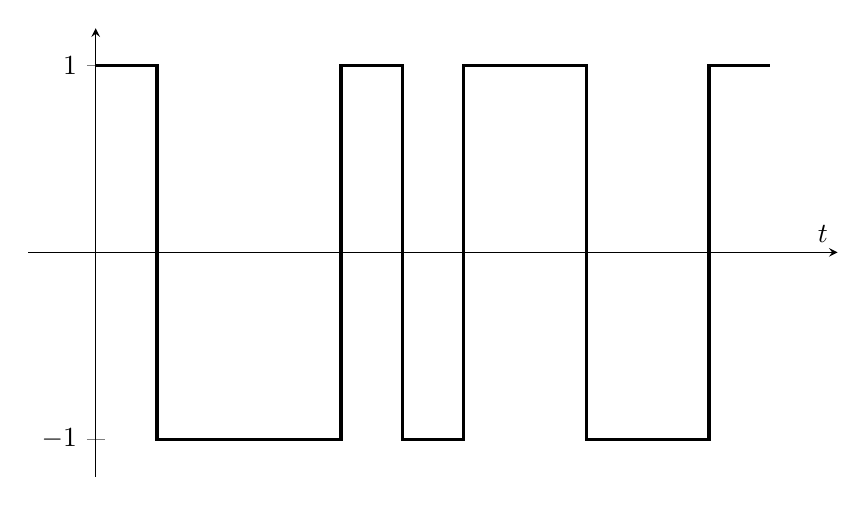
\begin{tikzpicture}
\begin{axis}[axis lines=middle,no markers,enlargelimits,xscale=1.5,xtick={0},xlabel={$t$},ytick={-1,1}]
\addplot [very thick]coordinates {(0,1)(1,1)(1,-1)(2,-1)(4,-1)(4,1)(5,1)(5,-1)(6,-1)(6,1)(8,1)(8,-1)(10,-1)(10,1)(11,1)};
\end{axis}\end{tikzpicture}
\end{figure}

Si calcola la probabilità che ad un dato istante $t$ la singola realizzazione abbia uno dei due valori:
\begin{equation}\begin{split}P(X(t)=1)=&P(X(t)=1|X(0)=1)P(X(0)=1)+\\&+P(X(t)=1|X(0)=-1)P(X(0)=-1)\end{split}\end{equation}
in cui la prima probabilità condizionata si ha per un numero di eventi pari di Poisson, mentre la seconda si ha per un numero di eventi dispari, ovvero
\begin{equation}\begin{split}P(X(t)=1|X(0)=1)&=\sum_{k=0}^{+\infty}{\frac{(\alpha t)^{2k}}{(2k)!}\e{-\alpha t}}=\\
&=\e{-\alpha t}\sum_{k=0}^{+\infty}{\frac{1}{2}\left[\frac{(\alpha t)^k}{k!}+\frac{(-\alpha t)^k}{k!}\right]}=\\
&=\frac{\e{-\alpha t}}{2}(\e{\alpha t}+\e{-\alpha t})=\frac{1}{2}(1+\e{-2\alpha t})
\end{split}\end{equation}
\begin{equation}\begin{split}P(X(t)=1|X(0)=-1)&=\sum_{k=0}^{+\infty}{\frac{(\alpha t)^{2k+1}}{(2k+1)!}\e{-\alpha t}}=\\
&=\e{-\alpha t}\sum_{k=0}^{+\infty}{\frac{1}{2}\left[\frac{(\alpha t)^k}{k!}-\frac{(-\alpha t)^k}{k!}\right]}=\\
&=\frac{\e{-\alpha t}}{2}(\e{\alpha t}-\e{-\alpha t})=\frac{1}{2}(1-\e{-2\alpha t})
\end{split}\end{equation}
da cui
\begin{equation}P(X(t)=1)=\frac{1}{2}\left[\frac{1}{2}(1+\e{-2\alpha t})+\frac{1}{2}(1-\e{-2\alpha t})\right]=\frac{1}{2}\end{equation}
Analogamente si ha $P(X(t)=-1)=\frac{1}{2} \implies$ \text{processo senza memoria}.

Si calcola la funzione valor medio e la funzione varianza del processo:
\begin{equation}\mu_X(t)=\E{X(t)}=\frac{1}{2}\cdot(-1)+\frac{1}{2}\cdot(+1)=0\end{equation}
\begin{equation}\sigma^2(t)=\E{X^2(t)}-0=\frac{1}{2}(-1)^2+\frac{1}{2}(+1)^2=1\end{equation}

La funzione di autocorrelazione e la funzione di autocovarianza, data la funzione valor medio, sono \[C_X(t_1,t_2)=R_X(t_1,t_2)=\E{X(t_1)X(t_2)}\]
il prodotto $X(t_1)X(t_2)$ può assumere solo due valori $+1$ o $-1$ a seconda del numero pari o dispari di arrivi nell'intervallo $[t_1,t_2[$, come si è visto con probabilità
\[\begin{split}P(X(t_1)X(t_2)=1)&=\frac{1}{2}(1+\e{-2\alpha(t_2-t_1)})\\
P(X(t_1)X(t_2)=-1)&=\frac{1}{2}(1-\e{-2\alpha(t_2-t_1)})\end{split}\]
pertanto si ha che
\begin{equation}\begin{split}\E{X(t_1)X(t_2)}=\frac{1}{2}\left[(+1)(1+\e{-2\alpha(t_2-t_1)})+(-1)(1+\e{-2\alpha(t_2-t_1)})\right]=\e{-2\alpha(t_2-t_1)}\end{split}\end{equation}
ovvero funzione autocorrelazione e autovarianza dipendono dalla differenza dei due istanti di tempo generici e non dagli istanti stessi.

\section{Processi stazionari}
I \textsc{processi stazionari} hanno la notevole proprietà di mantenere costanti i parametri statistici determinati in $X(t)$ e in $X(t+\Delta t)$. 

In generale si è visto che le funzioni densità di probabilità congiunta di ordine $n$ e i momenti di ordine $n$ dipendono dalla $n$-pla degli istanti di tempo $t_1,t_2,\dots,t_n$.

\subsection{Processo stazionario in senso stretto (SSS)}
Un processo aleatorio $X(t)$ è \textsc{stazionario in senso stretto (SSS)} se le funzioni densità di probabilità congiunta di ogni ordine siano invarianti ad una traslazione rigida degli istanti di tempo, ovvero che per ogni ordine $n$
\begin{equation}
\forall\Delta t\quad f_X(x_1,\dots,x_n;t_1,\dots,t_n)=f_X(x_1,\dots,x_n;t_1+\Delta t,\dots,t_n+\Delta t)
\end{equation}
Come corollario si ha che la stazionarietà di ordine $n$ implica la stazionarietà di ogni ordine inferiore.
Un processo stazionario in senso stretto ha quindi indici statistici che non distinguono il processo $X(t)$ dal processo $X(t+\Delta t)$.

Questo vuol dire ad esempio che la funzione densità di probabilità del primo ordine di un processo SSS è invariante rispetto al tempo $t$:
\[f_X(x;t)=f_X(x;t+\Delta t)\quad\forall\Delta t\]
Di conseguenza tutte gli indici statistici del primo ordine non dipendono dal tempo $t$:
\[\mu_X(t)=\mu_X\quad \sigma^2_X(t)=\sigma^2_X\]

Estraendo da un processo aleatorio stazionario in senso stretto di ordine 2 negli istanti di tempo $t_1$ e $t_2$ le variabili aleatorie $X(t_1)$ e $X(t_2)$ si ha la densità di probabilità congiunta
\[f_X(x_1,x_2;t_1,t_2)=f_X(x_1,x_2;t_1+\Delta t,t_2+\Delta t)\quad\forall\Delta t\]
ovvero la funzione densità di probabilità congiunta non dipende dagli istanti di tempo separatamente ma dalla differenza dei due
\begin{equation}
f_X(x_1,x_2;t_1,t_2)=f_X(x_1,x_2;t_1-t_2)
\end{equation}
Di conseguenza tutti gli indici statistici del secondo ordine, funzione autocorrelazione e autocovarianza, dipendono non dagli istanti di tempo ma dalla differenza $t_1-t_2$:
\[R_X(t_1,t_2)=R_X(t_1-t_2)\quad C_X(t_1,t_2)=C_X(t_1-t_2)\]

In generale la densità di probabilità congiunta e tutte le statistiche di ordine $n$ di un processo stazionario in senso stretto dipenderanno solo dalle differenze $t_1-t_2, t_2-t_3, \dots, t_{n-1}-t_n$, che restano invariate in una traslazione rigida dei tempi.

\begin{nota}Per gli scopi ingegneristici la richiesta di stazionarietà in senso stretto è di difficile applicazione perché raramente le funzioni densità di probabilità di ogni ordine sono date in forma chiusa (notevole eccezione sono i processi gaussiani). Inoltre raramente si è interessati ad indici statistici di ordine superiore a due.
\end{nota}

\subsection{Processo stazionario in senso lato (SSL)}
Una definizione di stazionarietà meno restrittiva e più semplice da verificare:

Un processo aleatorio $X(t)$ è \textsc{stazionario in senso lato} se
\begin{equation}\label{eq:processo_stazionario_senso_lato}
\begin{cases}
\mu_X(t)=\mu_X\\
R_X(t_1,t_2)=R_X(t_1-t_2)
\end{cases}
\end{equation}
La funzione di autocorrelazione si può scrivere, ponendo $t_1=t$ e $t_2=t-\tau$, come \begin{equation}R_X(t_1,t_2)=R_X(t,t-\tau)=\E{X(t)X(t-\tau)}=R_X(\tau)\end{equation}
In tal caso anche la funzione autocovarianza dipende da $\tau=t_1-t_2$
\begin{equation}C_X(t_1,t_2)=R_X(t_1-t_2)-\mu^2_X=R_X(\tau)-\mu^2_X\end{equation}

Non è richiesta alcuna proprietà di invarianza delle densità di probabilità che possono anche non essere conosciute in forma chiusa. 
La stazionarietà di ordine 2 è condizione sufficiente per avere un processo SSL.

La stazionarietà in senso lato non implica la stazionarietà in senso stretto.

\begin{esempio}
Si è visto un esempio di processo aleatorio non stazionario definito dall'oscillatore 
\[X(t)=a\cos{2\pi f_0 t+\theta}\]
con fase $\theta$ variabile aleatoria a distribuzione uniforme in $[0,\pi[$
di cui si è calcolata la funzione valor medio funzione del tempo $t$ (eq.\ref{eq:esempio_processo_non_stazionario_valor_medio})
\[\mu_X(t)=-\frac{2a}{\pi}\sen{2\pi f_0 t}\]
Il processo è non stazionario nonostante l'autocorrelazione (eq.\ref{eq:autocorrelazione_oscillatore_non_stazionario}) sia funzione di $t_1-t_2$.
\end{esempio}

\begin{esempio}\label{es:oscillatore_stazionario_senso_lato}
Esempio di processo aleatorio stazionario in senso lato è l'oscillatore 
\[X(t)=a\cos{2\pi f_0 t+\theta}\] 
con fase $\theta$ variabile aleatoria a distribuzione uniforme in $[0,2\pi[$
che ha funzione valor medio funzione $\mu_X(t)=0$, quindi non dipende da $t$ e funzione di autocorrelazione (eq.\ref{eq:autocorrelazione_oscillatore_stazionario}) che dipende solo da $t_1-t_2$:
\[R_X(t_1,t_2)=\frac{a^2}{2}\cos{2\pi f_0(t_1-t_2)}\]
\end{esempio}

\section{Processo telegrafico casuale: segnale dati}
Si supponga di avere un processo stocastico che modelli un segnale dati binario con frequenza di clock $\frac{1}{T}$ modello della trasmissione di bit tra due sistemi.

Le realizzazioni sono funzioni $V(t)$ che possano assumere solo due valori discreti $+1$ e $-1$ e i cambi di stato avvengono in istanti di tempo multipli interi di un periodo $T$.
\begin{equation}V_n=\begin{cases}
1&p=\frac{1}{2}\\-1&1-p=\frac{1}{2}
\end{cases}\end{equation}
I valori $V_n$ sono assunti in modo indipendente l'uno dall'altro e sono equiprobabili. La funzione si dice di \emph{sample and hold}: il segnale cambia di stato in istanti prefissati e mantiene costante il valore nell'intervallo di tempo tra transizioni successive $V(t)=V_n$ per $n T\leq t<(n+1)T$.
La funzione $V(t)$ è un treno di impulsi rettangolari scalati e traslati 
\begin{equation}\label{eq:segnale_dati}
V(t)=\sum_{n=-\infty}^{+\infty}{V_n\rect{\frac{t-n T-\frac{T}{2}}{T}}}
\end{equation}

Dall'osservazione dei valori assunti e dall'equiprobabilità si desume la funzione densità di probabilità del primo ordine:
\begin{equation}f_V(v;t)=\frac{1}{2}\impulse(v-1)+\frac{1}{2}\impulse(v+1)\end{equation}
La funzione densità di probabilità del primo ordine non dipende dal tempo quindi il processo è stazionario in senso stretto per il primo ordine. Infatti la funzione valor medio è costante
\begin{equation}\label{eq:segnale_binario_media}\mu_V(t)=\intinf{v f_V(v;t)}{v}=\intinf{\frac{1}{2}v\impulse(v-1)+\frac{1}{2}v\impulse(v+1)}{v}=\frac{1}{2}-\frac{1}{2}=0 \end{equation}

Il calcolo della funzione di autocorrelazione , indice statistico del secondo ordine, avviene per due istanti di tempo generici $t_1$ e $t_2$. Come si può vedere in figura nel grafico di una realizzazione i due istanti di tempo possono assumere gli stessi valori $V(t_1)=V(t_2)=V_n$ all'interno di uno stesso intervallo di tempo, per cui
\begin{equation}R_V(t_1,t_2)=\E{V(t_1)V(t_2)}=\E{V(t_1)}\E{V(t_2)}=\E{V_n^2}=1^2\cdot\frac{1}{2}+(-1)^2\cdot\frac{1}{2}=1\end{equation}
In un'altra coppia di istanti di tempo è possibile trovarsi nella condizione $V(t'_1)\neq V(t'_2)$, ad esempio a cavallo di due intervalli in cui è avvenuto un cambio di stato, per i quali
\begin{equation}R_V(t'_1,t'_2)=\E{V(t'_1)V(t'_2)}=\E{V(t'_1)}\E{V(t'_2)}=\left(1\cdot\frac{1}{2}-1\cdot\frac{1}{2}\right)^2=0\end{equation}
\begin{figure}[h!]
	\centering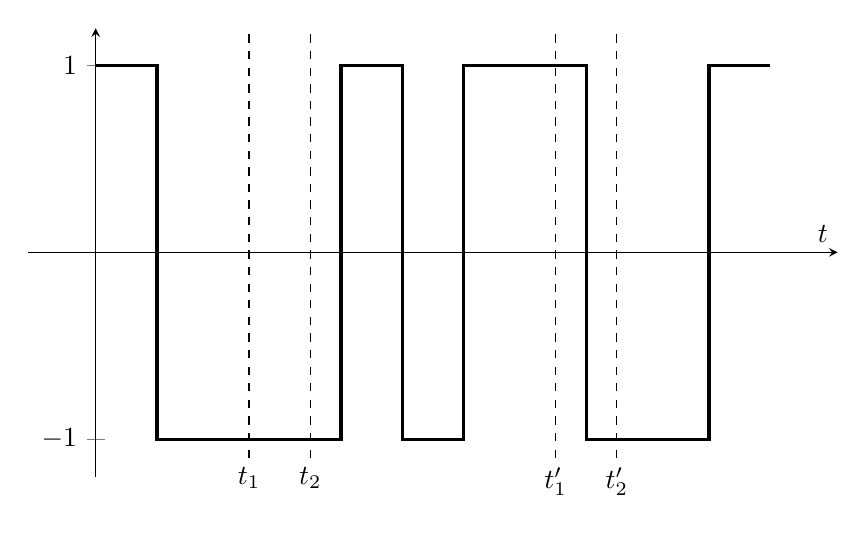
\begin{tikzpicture}
	\begin{axis}[axis lines=middle,no markers,enlargelimits,xscale=1.5,xtick={0},xlabel={$t$},ytick={-1,1},clip=false]
	\addplot [very thick]coordinates {(0,1)(1,1)(1,-1)(2,-1)(4,-1)(4,1)(5,1)(5,-1)(6,-1)(6,1)(8,1)(8,-1)(10,-1)(10,1)(11,1)};
	\draw [dashed] (axis cs:2.5,-1.1) node[below]{$t_1$} -- (axis cs:2.5,1.2)
	(axis cs:3.5,-1.1) node[below]{$t_2$} -- (axis cs:3.5,1.2);
	\draw [dashed] (axis cs:7.5,-1.1) node[below]{$t'_1$} -- (axis cs:7.5,1.2)
	(axis cs:8.5,-1.1) node[below]{$t'_2$} -- (axis cs:8.5,1.2);
	\end{axis}\end{tikzpicture}
\caption{Realizzazione di un processo dati binario}\label{fig:processo_dati_binario}
\end{figure}

Pertanto l'autocorrelazione dipende dai due istanti di tempo $t_1$ e $t_2$, questo implica che il processo non è stazionario in senso lato pur essendo stazionario in senso stretto per il primo ordine.

\section[Processo aleatorio con riferimento temporale aleatorio]{Processo aleatorio con riferimento temporale aleatorio: segnale eco radar}
Si modella il processo stocastico di un segnale di cui si conosce l'andamento ma il cui riferimento temporale è una variabile aleatoria $\theta$:
\begin{equation}X(t)=p(t-\theta)\end{equation}
Ad esempio il segnale può essere un segnale periodico di periodo $T$: $p(t)=p(t+T)$. La variabile aleatoria uniformemente distribuita in $[0,T]$.

Si determinano le proprietà del processo. La funzione valor medio, calcolata sulla trasformata della variabile aleatoria $\theta$ (che ha funzione densità $f_\Theta(\theta)=\frac{1}{T}\rect{\frac{t-T/2}{T}}$):
\[\mu_X(t)=\E{p(t-\theta)}=\intd{0}{T}{p(t-\theta)\frac{1}{T}}{\theta}=\frac{1}{T}\intd{t}{t-T}{-p(\alpha)}{\alpha}=\frac{1}{T}\intd{t-T}{t}{p(\alpha)}{\alpha}\]
dove si è posto $\alpha=t-\theta$, $\diff\alpha=-\diff\theta$, gli estremi di integrazione $\theta=0\to\alpha=t$, $\theta=T\to\alpha=t-T$.
L'integrale sulla funzione periodica su un intervallo di ampiezza $T$ non dipende dal valore $t$. Il valor medio statistico è pari al valor medio temporale della funzione $p(\alpha)$.

La funzione autocorrelazione
\[R_X(t_1,t_2)=\E{p(t_1-\theta)p(t_2-\theta)}=\frac{1}{T}\intd{0}{T}{p(t_1-\theta)p(t_2-\theta)}{\theta}=\]
cambio di variabile pongo $\alpha=t_1-\alpha$, $\diff\alpha=-\diff\theta$
\[=\frac{1}{T}\intd{t_1}{t_1-T}{-p(\alpha)p(t_2-t_1+\alpha)}{\alpha}=\frac{1}{T}\intd{t_1-T}{t_1}{p(\alpha)p(t_2-t_1+\alpha)}{\alpha}=R_X(t_1-t_2)\]
l'integranda è il prodotto di due termini periodici di periodo $T$, che è ancora di periodo $T$, quindi il suo integrale non dipende dal particolare istante iniziale di integrazione sul periodo. Pertanto la funzione autocorrelazione del processo $X(t)$ non dipende separatamente da $t_1$ e $t_2$ ma è funzione di $t_1-t_2$.

Essendo la funzione valor medio indipendente dal valor $t$ e la funzione autocorrelazione dipendente dal valore di $t_1-t_2$ il processo risulta stazionario in senso lato.

\clearpage
\section{Proprietà funzione autocorrelazione processo SSL}
Proprietà della funzione di autocorrelazione di un processo stazionario in senso lato:
\begin{enumerate}
\item La funzione di autocorrelazione è pari
\[R_X(\tau)=R_X(-\tau)\]
\begin{proof}[Dim.]
\[R_X(\tau)=\E{X(t)X(t-\tau)}=\E{X(t+\tau)X(t)}=R_X(-\tau)\]
\end{proof}

\item Il valore assunto da $R_X(\tau)$ nell'origine è pari alla potenza statistica del processo
\[R_X(0)=P_X=\E{X^2(t)}\]
\begin{nota}I processi aleatori SSL sono sempre segnali di potenza perché le varie realizzazioni che si estraggono da un processo non possono essere tutte infinitesime.\end{nota}

\item La funzione autocorrelazione è massima in modulo nell'origine
\[R_X(0)\geq\abs{R_X(\tau)}\]

\begin{proof}[Dim.]
\[\E{(X(t)\pm X(t-\tau))^2}\geq 0\]
disuguaglianza sempre vera perché aspettazione di una quantità sempre positiva, sviluppando la relazione
\begin{gather*}\E{X^2(t)}+\E{X^2(t-\tau)}\pm 2 \E{X(t)X(t-\tau)}\geq 0\\2R_X(0)\pm 2R_X(\tau)\geq 0\\R_X(0)\geq\pm R_X(\tau)\\ R_X(0)\geq\abs{R_X(\tau)}\end{gather*}
\end{proof}

\item Se $R_X(\tau)$ non è periodica allora \begin{equation}\lim\limits_{\tau\to\infty}R_X(\tau)=\mu^2_X\end{equation}
\begin{proof}[Dim.]
Per funzione di autocorrelazione che dipende solo dalla differenza dei tempi si ha che la funzione autocovarianza $C_X(\tau)=R_X(\tau)-\mu^2_X\xrightarrow{\tau\to\infty}0$ ovvero a crescere della distanza $\tau$ si hanno valori delle variabili aleatorie sempre meno correlati. La funzione di autocorrelazione pertanto $R_X(\tau)\xrightarrow{\tau\to\infty}\mu^2_X$.
\end{proof}
\end{enumerate}

\section[Processo aleatorio con riferimento temporale aleatorio]{Processo aleatorio: segnale dati binari}
Si considera nuovamente il segnale dati (eq.\ref{eq:segnale_dati}) con riferimento temporale non noto. Tale fenomeno si verifica ad esempio quando il ricevente riceve un segnale con un ritardo che dipende dalla distanza dal trasmittente. Un modello di questo processo con $\theta$ variabile aleatoria uniformemente distribuita in $[0,T]$, e valori $V_n$ indipendenti tra loro ed equiprobabili,
\[X(t)=V(t-\theta)=\sum_{n=-\infty}^{+\infty}V_n\rect{\frac{t-\theta-n T-T/2}{T}}\]
Come abbiamo visto il segnale telegrafico casuale ha funzione valor medio costante $\mu_X(t)=\mu_X=0$ (eq.\ref{eq:segnale_binario_media}).
Inoltre la funzione di autocorrelazione 
\[\begin{split}R_X(t_1,t_2)&=\E{X(t_1)X(t_2)}=\\
&=\E{\sum_{n=-\infty}^{+\infty}\sum_{m=-\infty}^{+\infty}V_n V_m\rect{\frac{t_1-\theta-n T-\frac{T}{2}}{T}}\rect{\frac{t_2-\theta-m T-\frac{T}{2}}{T}}}=\\
\intertext{essendo $\E{V_nV_m}\neq 0$ solo se $n=m$ la doppia sommatoria si riduce ad un elemento}
&=\sum_{n=-\infty}^{+\infty}\frac{1}{T}\intd{0}{T}{\rect{\frac{t_1-\theta-n T-T/2}{T}}\rect{\frac{t_2-\theta-m T-T/2}{T}}}{\theta}=\\
\intertext{cambio di variabili $t_1=t, t_2=t-\tau, \alpha=t-\theta-n T,\diff\alpha=-\diff\theta, \theta=0\to\alpha=t-nT, \theta=T\to t-(n+1)T$, inverto gli estremi per il segno di $-\diff\theta$}
&=\frac{1}{T}\sum_{n=-\infty}^{+\infty}\intd{t-n T-T}{t-n T}{\rect{\frac{\alpha-T/2}{T}}\rect{\frac{\alpha-\tau-T/2}{T}}}{\alpha}=\\
\intertext{l'integranda non dipende da $n$, la sommatoria degli integrali su intervalli disgiunti $[n T-T,n T]$ può essere sostituita da un unico integrale}
&=\frac{1}{T}\intd{-\infty}{+\infty}{\rect{\frac{\alpha-T/2}{T}}\rect{\frac{\alpha-\tau-T/2}{T}}}{\alpha}=\\
&=\frac{1}{T}\rect{\frac{\tau-T/2}{T}}\ast\rect{\frac{-\tau-T/2}{T}}
\end{split}\]
La funzione autocorrelazione dipende dalla sola variabile $\tau$ e rappresenta una correlazione deterministica convoluzione di due funzioni rettangolo che è pari ad una funzione triangolare.
Il segnale dati binario con ritardo casuale, pertanto, è un processo stazionario in senso lato.

\section{Significato funzione autocorrelazione processo SSL}
Presi due processi stocastici stazionari in senso lato $X(t)$ e $Y(t)$, dotati degli stessi parametri statistici del primo ordine (funzione valor medio, funzione potenza, funzione varianza), ad esempio con valor medio $\mu_X(t)=\mu_Y(t)=\text{costante}$. Per poter distinguere statisticamente i segnali si analizzano i parametri statistici del secondo ordine (funzione autocorrelazione, funzione autocovarianza).
Supponendo che $R_X(\tau)\neq R_Y(\tau)$ ho modo di distinguere i processi.
In particolare quello che si osserva per istanti di tempo distanti $\tau$ è una diversa velocità di variazione: infatti uno dei due segnali assomiglierà di più a se stesso (autocorrelazione maggiore), ovvero le variazioni delle realizzazioni sono più lente e quindi più somiglianti tra loro.

\section{Filtraggio processo aleatorio}
La teoria dei processi stocastici modella fenomeni reali descrivibili da grandezze fisiche che variano nel tempo in modo non predicibile a priori. Essendo le grandezze fisiche manipolabili ha senso chiedersi cosa significa filtrare un processo aleatorio attraverso un sistema.

In particolare per sistemi lineari tempo-invarianti si avrà che un segnale $x(t)$ in ingresso al sistema sarà convoluto con la risposta all'impulso del sistema per avere in uscita un segnale $y(t)=x(t)\ast h(t)$.

Nei processi aleatori avremo usualmente un segnale deterministico noto a cui è sovrapposto un segnale di disturbo o rumore che è modellato dal processo aleatorio a valor medio nullo. Compito dell'ingegnere è progettare filtri che eliminino, almeno in parte, la componente rumorosa dalle realizzazioni del processo.

\begin{figure}[h!]\centering
	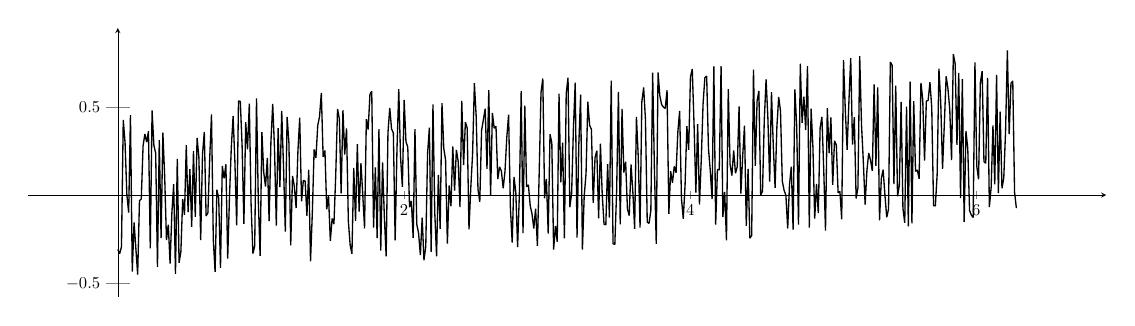
\begin{tikzpicture}[scale=.6]
	\begin{axis}[axis lines=middle,no markers,enlargelimits,xscale=3.33,line join=bevel]
	\addplot [thick,domain=0:6.28,samples=500] {sin(pi*x+0.5)+.5*rand};
	\end{axis}\end{tikzpicture}
	\caption{Esempio di segnale deterministico affetto da rumore}
\end{figure}

Per ogni realizzazione $x(t;\omega)$ del processo $X(t)$ dello spazio campione $\Omega$ si otterrà in uscita dal sistema filtro una funzione $y(t)=x(t;\omega)\ast h(t)$. L'insieme dei segnali di uscita costituisce un nuovo processo, $Y(t)$ che indichiamo con
\begin{equation}
Y(t)=X(t)\ast h(t)
\end{equation}

\begin{figure}[!h]\centering
	\begin{tikzpicture}[node distance=3cm]
	\node [block] (system) at (0,0) {$h(t)$};
	\node [left of=system](input) {};
	\node [right of=system] (output) {};
	\draw [-latex] (input) -- (system) node[pos=.5,above]{$X(t)$};
	\draw [-latex] (system) -- (output) node[pos=.5,above]{$Y(t)$};
	\end{tikzpicture}
	\caption{Filtraggio del processo $X(t)$}
\end{figure}

Generalmente il problema di determinare la funzione densità di probabilità congiunta di qualunque ordine per il processo d'uscita, ammesso che sia nota quella del processo di ingresso, è insolubile.

Si determina allora la relazione dei parametri statistici di primo e secondo ordine in ingresso, almeno la funzione valor medio e la funzione autocorrelazione di $X(t)$, e i corrispondenti dell'uscita.

\begin{equation}
\begin{split}
\mu_Y(t)&=\E{Y(t)}=\E{X(t)\ast h(t)}=\E{\intinf{h(\tau)X(t-\tau)}{\tau}}=\\
&=\intinf{\E{h(\tau)X(t-\tau)}}{\tau}=\intinf{h(\tau)\E{X(t-\tau)}}{\tau}=\\
&=\intinf{h(\tau)\mu_X(t-\tau)}{\tau}=\\
&=\mu_X(t)\ast h(t)
\end{split}
\end{equation}
Il risultato $\mu_Y(t)=\mu_Y(t)\ast h(t)$ è notevole: la funzione valor medio in uscita si ottiene come convoluzione della funzione valor medio in ingresso con la risposta all'impulso del sistema. Pertanto un sistema con in ingresso un segnale deterministico a cui si somma un processo stocastico a valor medio nullo, per la linearità del sistema, darà in uscita un processo somma di una componente deterministica e di una componente statistica che avrà ancora valor medio nullo. Il filtraggio ottimo elimina la componente statistica e preserva la componente deterministica.
\begin{equation}
\underset{\text{proc.aleat.}}{X(t)} = \underset{\text{proc.aleat. a media nulla}}{X_0(t)} + \underset{\text{segn.determ.}}{\mu_x(t)} 
\end{equation}

La funzione autocorrelazione in uscita
\begin{equation}
\begin{split}
R_Y(t_1,t_2)&=\E{Y(t_1)Y(t_2)}=\E{(X(t_1)\ast h(t_1))\cdot(X(t_2)\ast h(t_2))}=\\
&=\E{\intinf{\intinf{X(\alpha)h(t_1-\alpha)X(\beta)h(t_2-\beta)}{\alpha}}{\beta}}=\\
&=\intinf{\intinf{h(t_1-\alpha)h(t_2-\beta)\E{X(\alpha)X(\beta)}}{\alpha}}{\beta}=\\
&=\intinf{\intinf{h(t_1-\alpha)h(t_2-\beta)R_X(\alpha,\beta)}{\alpha}}{\beta}=\\
&=R_X(t_1,t_2)\ast h(t_1)\ast h(t_2)
\end{split}
\end{equation}

\section{Filtraggio processo stazionario in senso lato}\label{sec:filtraggio_processo_SSL}
Si ha in ingresso al filtro un processo stazionario in senso lato, che ha funzione valor medio costante e funzione di autocorrelazione dipendente da $\tau=t_1-t_2$ (eq.\ref{eq:processo_stazionario_senso_lato}).

La funzione valor medio in uscita
\begin{equation}
\mu_Y(t)=\mu_X(t)\ast h(t)=\intinf{h(\tau)\mu_X(t-\tau)}{\tau}=\mu_X\intinf{h(\tau)}{\tau}=\mu_X\cdot \restrict{H(f)}{f=0}=\text{cost}
\end{equation}
dove $H(0)$ è il valore della trasformata di Fourier della risposta all'impulso nell'origine, e la funzione valor medio in uscita assume valore costante.

La funzione di autocorrelazione in uscita
\begin{equation}\begin{split}
R_Y(t,t-\tau)&=\E{Y(t)Y(t-\tau)}=\E{(X(t)\ast h(t))(X(t-\tau)\ast h(t-\tau))}=\\&=\E{\intinf{\intinf{h(\alpha)X(t-\alpha)h(\beta)X(t-\tau-\beta)}{\alpha}}{\beta}}=\\&=\intinf{\intinf{h(\alpha)h(\beta)\E{X(t-\alpha)X(t-\tau-\beta)}}{\alpha}}{\beta}=\\&=\intinf{\intinf{h(\alpha)h(\beta)R_X(\tau+\beta-\alpha)}{\alpha}}{\beta}=\\
\intertext{si può osservare che la funzione di autocorrelazione non dipende da $t$ ma solo da $\tau$ pertanto filtrando un processo stazionario si ottiene un processo stazionario,}
&=\intinf{h(\beta)\underbrace{\left[\intinf{R_X(\tau+\beta-\alpha)h(\alpha)}{\alpha}\right]}_{R_X(\tau+\beta)\ast h(\tau+\beta)=g(\tau+\beta)}}{\beta}=\\
&=\intinf{h(\beta)g(\tau+\beta)}{\beta}=\intinf{h(-z)g(\tau-z)}{z}=g(\tau)\ast h(-\tau)
\end{split}
\end{equation}
Si ottiene quindi
\begin{equation}
R_Y(\tau)=R_X(\tau)\ast h(\tau)\ast h(-\tau)=R_X(\tau)\ast R_h(\tau)
\end{equation}
dove la convoluzione del segnale $h(\tau)\ast h(-\tau)$ è l'autocorrelazione del segnale deterministico risposta all'impulso.

Un processo stazionario in senso lato in ingresso ad un sistema lineare tempo invariante viene filtrato e da in uscita un processo stazionario in senso lato.

Il filtraggio di un processo aleatorio $X(t)$ ha quindi due casi per cui la funzione valor medio e di autocorrelazione del processo in uscita sono legate a quelle del processo in ingresso

\begin{table}[!h]
\centering
\begin{tabular}{c|c}
\toprule
\multicolumn{2}{c}{$Y(y)=X(t)\ast h(t)$} \\
\midrule
caso $X(t)$ generico & caso $X(t)$ SSL  \\ 
$\begin{cases}
\mu_Y(t)=\mu_X(t)\ast h(t)\\R_Y(t_1,t_2)=R_X(t_1,t_2)\ast h(t_1)\ast h(t_2)
\end{cases}$ & $\begin{cases}
\mu_Y(t)=\mu_X\cdot H(0)\\R_Y(\tau)=R_X(\tau)\ast R_h(\tau)
\end{cases}$ \\ 
\bottomrule
\end{tabular} 
\end{table}


\chapter{Analisi spettrale dei processi aleatori}
Si è data una descrizione del problema del filtraggio di un processo aleatorio, e il calcolo delle statistiche di primo e secondo ordine, per un sistema lineare stazionario in ambito temporale.

Ha senso analizzare in frequenza la risposta di un sistema lineare tempo invariante ad un processo aleatorio $X(t,\omega)$ e ad una analisi di Fourier delle realizzazioni, i segnali $x(t)$ estratti dal processo.

Ci si limiterà qui a studiare le proprietà in frequenza per soli processi aleatori stazionari in senso lato. L'analisi di Fourier di un processo richiederebbe lo studio in frequenza di ampiezza e fase dello spettro di ogni realizzazione del processo, e delle relazioni tra gli indici statistici nel tempo e in frequenza.
\`{E} comune limitarsi alla descrizione degli spettri di potenza del segnale aleatorio.

Le funzioni campione di un processo stazionario non possono essere segnali a energia finita, perché andando asintoticamente a zero la funzione valor medio tenderebbe a zero per tutte le funzioni campione, mentre in generale i processi SSL hanno media costante (non necessariamente nulla).
In generale le funzioni campione di un processo stazionario sono segnali a potenza finita, perciò il processo aleatorio ammette spettro di potenza.

La funzione densità spettrale di potenza di un processo aleatorio è la media delle funzioni densità spettrale di potenza ottenute per le realizzazioni
\begin{equation}
S_X(f,\omega)=\E{S_X(f;\omega)}
\end{equation}

Lo spettro di potenza del processo come valor medio dello spettro di potenza delle funzioni campione
\begin{equation}\label{eq:densita_spettrale_processo_aleatorio}S_X(f)=\E{\lim\limits_{t\to+\infty}\frac{X_T(f)^2}{T}}=\E{\lim\limits_{t\to+\infty}\frac{\abs{\fourier{x_T(t;\omega)}}^2}{T}}\end{equation}
dove la trasformata di Fourier si applica al segnale $x(t)$ troncato all'intervallo $[-\frac{T}{2},\frac{T}{2}]$.
Questa definizione, valida anche per processi non stazionari, è molto difficile da utilizzare.

\section{Teorema di Wiener-Kintchine}
La densità spettrale di potenza dei processi stazionari in senso lato è calcolabile come trasformata di Fourier della funzione di autocorrelazione
\begin{equation}
S_X(f)=\fourier{R_X(\tau)}=\intinf{R_X(\tau)\e{-\imath 2\pi f\tau}}{\tau}
\end{equation}
Proprietà:
\begin{enumerate}
\item La densità spettrale è non negativa per definizione eq.\ref{eq:densita_spettrale_processo_aleatorio}: $S_X(f)\geq 0$
\item La densità spettrale di potenza di un processo aleatorio stazionario in senso lato è una funzione reale e pari.
\begin{proof}[Dim.]
Si ricorda che $R_X(\tau)=R_X(-\tau)$ è pari pertanto posso sommare i contributi nell'integrale
\[\intinf{R_X(\tau)\e{-\imath 2\pi f\tau}}{\tau}=\intd{0}{\infty}{R_X(\tau)\e{-\imath 2\pi f\tau}+R_X(-\tau)\e{+\imath 2\pi f\tau}}{\tau}=\intd{0}{\infty}{R_X(\tau)2\cos{2\pi f\tau}}{\tau}\]
\end{proof}
\item La potenza media statistica del processo, costante per processo stazionario, è pari all'integrale della densità spettrale di frequenza 
\begin{equation}
P_X=R_X(0)=\E{X^2(t)}=\intinf{S_X(f)}{f}
\end{equation}
\end{enumerate}

\section{Filtraggio processo stazionario}
Si può caratterizzare la densità spettrale del processo in uscita ad un sistema lineare tempo invariante nota la densità spettrale del processo in ingresso.
\`{E} noto che se il processo in ingresso è stazionario in senso lato lo è anche il processo in uscita.

La densità spettrale del processo in uscita
\begin{equation}
S_Y(f)=\fourier{R_X(\tau)\ast h(\tau)\ast h(-\tau)}=S_X(f)\cdot H(f)\cdot H(-f)
\end{equation}

Per sistemi reali la risposta all'impulso è una funzione reale, $H(-f)=\conj{H}(f)$
\begin{equation}
S_Y(f)=S_X(f)\cdot\abs{H(f)}^2
\end{equation}
che è la stessa relazione che vale per gli spettri di potenza dei segnali deterministici.
La risposta in fase del sistema non influenza la densità spettrale del processo in uscita.

Nella densità spettrale di potenza sono contenute tutte le informazioni spettrali del processo, ovvero come è distribuita la potenza alla varie frequenze. Il significato di densità spettrale di potenza è lo stesso per segnali deterministici e per processi aleatori.

\begin{esempio}
Si calcoli la densità spettrale di potenza del processo aleatorio stazionario \[X(t)=a\sen{2\pi f_0 t+\theta}\] con $\theta$ v.a. uniformemente distribuita in $[0,2\pi[$. Si è calcolata la funzione di autocorrelazione
\[R_X(\tau)=\frac{a^2}{2}\cos{2\pi f_0\tau}\]
Secondo la definizione di Wiener-Kintchine si può calcolare la densità spettrale può essere calcolata come
\[S_X(f)=\fourier{R_X(\tau)}=\frac{a^2}{4}[\impulse(f-f_0)+\impulse(f+f_0)]\]
\begin{figure}[h!]
	\centering\begin{tikzpicture}
	\draw [-latex] (-3,0)--(3,0) node[below] {$f$};
	\draw [-latex] (0,0)--(0,1.5) node[right] {$S_X(f)$};;
	\draw [very thick,-latex] (-2,0)--(-2,1);
	\draw [very thick,-latex] (2,0)--(2,1);
	\draw (-2,0) -- (-2,-1mm) node [below] {$-f_0$};
	\draw (0,0) -- (0,-1mm) node [below] {$0$};
	\draw (2,0) -- (2,-1mm) node [below] {$f_0$};
	\end{tikzpicture}
\end{figure}
\end{esempio} 

\begin{nota}
Poiché la densità spettrale di potenza è la trasformata di Fourier della funzione di autocorrelazione per processi stazionari si ha che tanto più rapidamente variano le singole realizzazioni di un processo, tanto più larga è la banda passante della densità spettrale di potenza. In altre parole a variazioni rapide corrispondono termini spettrali a potenza non nulla a frequenze più alte.\end{nota}

\section{Processo stocastico gaussiano}
Un processo aleatorio $X(t)$ è gaussiano se, presi $n$ istanti di tempo distinti, le variabili aleatorie $X_1(t),X_2(t),\dots,X_n(t)$ risultano congiuntamente gaussiane.
$X(t)$ è gaussiano se la densità di probabilità congiunta del vettore delle variabili aleatorie ha la forma
\begin{equation}
f_\vect{X}(x_1,\dots,x_n;t_1,\dots,t_n)=\frac{1}{\sqrt{(2\pi)^n\det\abs{ C_\vect{X}}}}\;\e{-\frac{1}{2}\trasp{(\vect{x}-\mu_\vect{X})}C^{-1}_\vect{X}(\vect{x}-\mu_\vect{X})}
\end{equation}
Per la conoscenza completa della funzione di densità di probabilità congiunta, e quindi dell'intero processo, è necessario conoscere la funzione valor medio del vettore $\vect{X}$, $\mu_\vect{X}(t)$, e la funzione di autocovarianza, la matrice $C_\vect{X}$ (si veda es.\ref{es:v_a_congiuntamente_gaussiane}) per ogni $n$-pla di istanti di tempo $(t_1,t_2,\dots,t_n)$. Si ricorda che la funzione valor medio del vettore delle variabili aleatorie è
\[\mu_\vect{X}(t)=\trasp{[\mu_X(t_1),\mu_X(t_2),\dots,\mu_X(t_n)]}\]
e gli elementi della matrice di covarianza si calcolano come 
\[c_{ij}=\E{(X(t_i)-\mu_X(t_i))\cdot (X(t_j)-\mu_X(t_j))}=C_X(t_i,t_j)=R_X(t_i,t_j)-\mu_X(t_i)\mu_X(t_j)\]

Per i processi gaussiani si ha la notevole proprietà per cui la stazionarietà in senso lato implica la stazionarietà in senso stretto. Questo perché la funzione densità di probabilità congiunta del processo dipende dalla funzione valor medio, che è costante, e dalla funzione di autocorrelazione, che dipende solo dalla differenza tra gli istanti di tempo ($\mu_X(t)=\mu_X$ e $R_X(t_1,t_2)=R_X(\tau)$), e quindi la stessa funzione di autocovarianza.

I processi gaussiani in ingresso a sistemi lineari tempo invarianti vengono filtrati e risultano ancora processi gaussiani in uscita.
\begin{proof}[Dim.]
\[Y(t)=X(t)\ast h(t)=\intinf{x(\alpha)h(t-\alpha)}{\alpha}\]
L'operazione di integrale si può pensare come somma di infiniti termini $X(k\Delta\alpha)h(t-k\Delta\alpha)\Delta\alpha$. Il processo in uscita risulta una combinazione lineare di tanti processi in ingresso tutti gaussiani pertanto è esso stesso gaussiano.
\end{proof}

\section{Processo aleatorio bianco}
Si supponga un modello teorico di un processo con densità spettrale di potenza la cui banda tende a crescere illimitatamente, mantenendo il valore presente in $f=0$. La densità spettrale di potenza del processo $X(t)$ tende a diventare costante a tutte le frequenze
\[S_X(f)=\xi\]
Il tempo di correlazione tende a ridursi fino ad arrivare al limite ad una funzione di autocorrelazione impulsiva
\[R_X(\tau)=\xi\impulse(\tau)\]
Il valore medio 
\[\mu_X(t)=\lim\limits_{\tau\to +\infty}R_X(\tau)=\mu^2_X=0\]

\begin{nota}Il processo aleatorio bianco è solo una astrazione matematica: uno spettro reale non potrà mai avere potenza a tutte le frequenze, avrebbe potenza infinita.\end{nota}

\subsection{Esempio resistore con rumore termico}
\begin{esempio}
L'agitazione termica degli elettroni in un resistore causa una tensione di rumore a vuoto proporzionale alla temperatura del componente. Rispetto al modello ideale si ha quindi un resistore con in serie un generatore di tensione pari a quella prodotta dal rumore termico. Quest'ultimo può essere modellato come un processo aleatorio stazionario.

\begin{figure*}[h]
	\centering\begin{circuitikz}[american voltages]
		\draw (0,0)	to[V,v^>=${N(t)}$] (0,3)
		to[R,l=${R}$] (2,3)
		to[open,*-*] (2,0) -- (0,0);
	\end{circuitikz}
\end{figure*}

La descrizione del fenomeno del rumore termico coinvolge considerazioni di meccanica quantistica che portano a determinare l'espressione della densità spettrale di potenza della tensione di rumore (formula di Nyquist)

\begin{equation}
S_N(f)=2 R \frac{\frac{\abs{f}}{f_0}}{\e{\frac{\abs{f}}{f_0}-1}}
=2 R \frac{\hbar\abs{f}}{\e{\frac{\hbar\abs{f}}{k_B T_R}-1}} \quad[\si{\volt\squared\per\hertz}]
\end{equation}

dove $f_0=\frac{k_B T_R}{\hbar}$, con la costante di Boltzmann $k_B=\SI{1.38e-23}{\joule\per\kelvin}$, la costante di Planck $\hbar=\SI{6.63e-34}{\joule\second}$, la temperatura ambiente $T_R=\SI{293}{\kelvin}$.
A temperatura ambiente la frequenza $f_0\cong\SI{6}{\tera\hertz}$

A frequenze $f\ll f_0$ posso approssimare
\[\e{\frac{\hbar\abs{f}}{k_B T_R}}-1\cong\frac{\hbar\abs{f}}{k_B T_R}\]
essendo $\e{x}=1+x+\frac{x^2}{2}+\dots$ la serie per $x\to 0$ si approssima $\e{x}\cong 1+x\implies\e{x}-1\cong x$.
\[S_N(f)= 2 R k_B T_R\]

La tensione quadratica media misurata con un voltmetro di banda $B$ è pari alla densita spettrale di potenza monolatera 
\[S_N^m(f)=4 R K_B T_R\]

Il modello del rumore bianco pertanto è utile: per calcolare gli effetti del rumore termico sull'uscita di un sistema filtrante si può sostituire la densità di potenza del rumore termico $S_N(f)$ con il suo modello semplificato di valore costante.
\end{esempio}

\begin{nota}Nel dimensionamento dei sistemi di telecomunicazione è importante la potenza trasmessa alla quale si somma la potenza del rumore. Si progettano i sistemi in modo da massimizzare la potenza trasmessa utile.
\end{nota}
\begin{figure*}[h]
\centering
\begin{circuitikz}[american voltages]
	\draw (0,0)	to[V,v^>=${v_n(t)}$] (0,3)
	to[R,l=${R}$,-*] (3,3)--(4,3)
	to[R,l=${R_L}$,v=${v_L(t)}$] (4,0) to[short,-*] (3,0)--(0,0);
	\draw node at(7,1.5) {$v_L(t)=\frac{R_L}{R+R_L}v_N(t)$}; 
\end{circuitikz}
\end{figure*}
La massima potenza in uscita $P(t)$ misurata in $\si{\watt}$ si ha quando il carico (\emph{Load}) è adattato, ovvero per $R_L=R$
\[P(t)=v_L(t)\cdot i(t)=v_L(t)\frac{v_N(t)}{R+R_L}=\frac{R_L}{R+R_L}v_N(t)\frac{v_N(t)}{R+R_L}\overset{R_L=R}{=}\frac{1}{2}\frac{v^2_N(t)}{2 R}\]
La densità spettrale monolatera di rumore disponibile in uscita in una banda $B$
\[\E{\frac{v^2_N(t)}{4 R}}=\frac{1}{4 R}\E{v^2_N(t)}=\frac{1}{4 R}4 R k_B T B=k_B T B \si{\watt\per\hertz}\]

\section{Esempio filtro passa basso con rumore termico}
\begin{esempio}
Esempio filtro passa basso con rumore termico.

\begin{figure*}[h]
	\centering\begin{circuitikz}[american voltages]
		\draw (0,0)	to[V,v^>=${V_S(t)}$] (0,3)
		to[R,l=${R}$,-*] (3,3)--(4,3)
		to[C,l=${C}$,v=${v_c(t)}$] (4,0) to[short,-*] (3,0)--(0,0);
	\end{circuitikz}
\end{figure*}

Trasformata della risposta all'impulso del sistema passa basso:
\[H(f)=\frac{V_c(f)}{V_n(f)}=\frac{1}{1+\imath 2\pi R C f}\]
La frequenza di taglio \[f_0=\frac{1}{2\pi R C}\]
Potenza media di rumore sulla resistenza
\[P_n(f)=2 R k_B T [\si{\volt\squared\per\hertz}]\]
Potenza media di rumore sul condensatore
\[P_{V_c}(f)=2 R k_B T \frac{1}{1+4\pi^2 R^2 C^2 f^2} [\si{\volt\squared\per\hertz}]\]

Calcolo la potenza media bilatera
\[\begin{split}\E{V_c^2}&=\intd{0}{+\infty}{\frac{4 R k_B T}{1+4\pi^2 R^2 C^2 f^2}}{f}=\\
\intertext{cambio variabile $\alpha=2\pi R C f$, $\diff\alpha=2\pi R C\diff f$}
&=\intd{0}{+\infty}{\frac{4 R k_B T}{2\pi R C}\frac{1}{1+\alpha^2}}{\alpha}=\bound{0}{+\infty}{\frac{4 k_B T}{2\pi C}\arctg\alpha}=\frac{4 k_B T}{2\pi C}\frac{\pi}{2}=\frac{k_B T}{C}
\end{split}\]
\end{esempio}

\begin{esempio}
Si hanno due resistenze in serie a diverse temperature. 

\begin{figure*}[!h]
	\centering
	\begin{circuitikz}[american voltages]
		\draw (0,6)	to[R,l={$R_1$},v=${v_{n_1}(t)}$] (0,3)
		to[R,l={$R_2$},v=${v_{n_2}(t)}$] (0,0)
		(0,6) to[short,-*] (3,6)
		to[open,-*,v=${v_n(t)}$] (3,0)--(0,0);
	\end{circuitikz}
\end{figure*}

La tensione di uscita è pari alle tensioni di rumore
\[v_n(t)=v_{n_1}(t)+v_{n_2}(t)\]

Sono tensioni a media nulla quindi posso sommare media e varianza.

\[\E{V^2_n}=\E{V^2_{n_1}}+\E{V^2_{n_2}}=\intinf{P_{n_1}(f)}{f}+\intinf{P_{n_2}(f)}{f}=\intinf{P_n(f)}{f}\]

La densità di potenza monolatera
\[P_n(f)=2 R_1 k_B T_1 + 2 R_2 k_B T_2\]

La densità di potenza bilatera
\[P_n^m(f)=4 R_1 k_B T_1 + 4 R_2 k_B T_2 = 4 R_\text{eq} k_B T_\text{eq}\]
dove la resistenza equivalente alla serie è $R_\text{eq}=R_1+R_2$ e la temperatura equivalente è data da
\[T_\text{eq}=\frac{T_1 R_1+T_2 R_2}{R_1+R_2}\]
\end{esempio}

\section{Rumore passa banda o a banda stretta}

Si suppone un processo aleatorio stazionario $X(t)=\mu_X(t)+N(t)$ somma di un segnale deterministico più un rumore a valor medio nullo che attraversa un filtro passa banda ideale, per modulazione del segnale.

Il rumore ha le seguenti proprietà:
\begin{enumerate}
\item Il rumore gaussiano bianco può essere rappresentato nelle sue componenti
\[N(t)=N_I(t)\cos{2\pi f_0 t}-N_Q(t)\sen{2\pi f_0 t}\]
dove $N_I(t)$ è la componente in fase del rumore e $N_Q(t)$ è la componente in quadratura.

\item $N_I(t)$ e $N_Q(t)$ sono processi aleatori passa basso $\abs{f}\leq B$

\item In uscita la potenza media a frequenza zero è nulla pertanto non ho potenza in continua. 

\item Le componenti $N_I$ e $N_Q$ hanno valor medio nullo.

\item Se $N(t)$ è gaussiano anche le componenti $N_I$ e $N_Q$ sono gaussiane.

\item Se $N(t)$ è stazionario anche le componenti $N_I$ e $N_Q$ sono stazionarie.

\item La densità spettrale di potenza delle componenti in uscita è
\[S_{N_I}(f)=S_{N_Q}(f)=\begin{cases}S(f-f_0)+S(f+f_0)&\abs{f}<B\\0&\text{altrimenti}\end{cases}\]

\item La varianza $\sigma^2_{N_I}=\sigma^2_{N_Q}=\sigma^2_N$
\end{enumerate}

\section{Sistema di filtraggio di rumore bianco su portante aleatoria}
\begin{figure}[h]\centering
	\begin{tikzpicture}[node distance=2cm]
	\node [block] (integrator) at (0,0) {$g(t)$};
	\node [left of=integrator](input) {$N(t)$};
	\node [sum,cross,right of=integrator,node distance=3cm] (mult) {}; 
	\node [below of=mult](modulator) {$p(t)$};
	\node [block,right = of mult] (filter) {$H(f)$};
	\node [right of=filter] (output) {$Z(t)$};
	\draw [-latex] (input) -- (integrator);
	\draw [-latex] (integrator) -- (mult) node[pos=.5,above]{$X(t)$};
	\draw [-latex] (modulator) -- (mult);
	\draw [-latex] (mult) -- (filter) node[pos=.5,above]{$Y(t)$};
	\draw [-latex] (filter) -- (output);
	\end{tikzpicture}
\end{figure}

Nel sistema illustrato si ha
\begin{itemize}
\item il processo aleatorio $N(t)$ stazionario in senso lato con densità spettrale costante di rumore bianco $S_n(f)=n$
\item filtro integratore a finestra mobile
\[g(t)=\frac{1}{T}\rect{\frac{t-\frac{T}{2}}{T}}\]
\item è un segnale portante 
\[p(t)=2\cos{2\pi f_0+\theta}\]
con fase $\theta$ variabile aleatoria uniformemente distribuita in $[0,2\pi[$
\item filtro passa banda ideale $H(f)$
\end{itemize}

Il processo $X(t)$ è stazionario in senso lato perché risulta il filtraggio di un sistema LTI di un processo rumore bianco, quindi SSL. 

La funzione valor medio $\mu_X(t)$ ha valore nullo perché la funzione valor medio $\mu_N(t)=0$ è identicamente nulla (rumore bianco).

La funzione di autocorrelazione \[R_X(\tau)=R_N(\tau)\ast g(\tau)\ast g(-\tau)=n\impulse(\tau)\ast R_g(\tau)= \frac{n}{T}\left(1-\frac{\abs{\tau}}{T}\right)\rect{\frac{\tau}{2T}}\]
che è l'espressione di un triangolo di altezza $\frac{1}{T}$ base $2T$ e pendenza $\frac{\abs{\tau}}{T}$

La densità spettrale di potenza
\[S_X(f)=n \abs{\fourier{g(t)}}^2=n\abs{G(f)}^2=n\Sinc^2(T f)\]

La portante è un processo aleatorio stazionario in senso lato (oscillatore es.\ref{es:oscillatore_stazionario_senso_lato}) con valor medio $\mu_p(t)=0$ e funzione di autocorrelazione 
\[R_X(\tau)=2\cos{2\pi f_0(\tau)}\]

Il processo prodotto $Y(t)$ avrà ancora valor medio nullo
\[\mu_Y(t)=\E{Y(t)}=\E{X(t)P(t)}=2 \E{X(t)\cos(2\pi f_0 t+\theta)}\]
la variabile aleatoria $\theta$ è indipendente dal processo $N(t)$, e quindi da $X(t)$, pertanto
\[\mu_Y(t)=\E{X(t)}\E{P(t)}=0\]
La funzione autocorrelazione di $Y(t)$ 
\[\begin{split}R_Y(\tau)&=\E{Y(t)Y(t-\tau)}=\\&=\E{X(t)2\cos{2\pi f_0 t+\theta} X(t-\tau)2\cos{2\pi f_0 (t-\tau)+\theta}}=\\
&=2 R_X(\tau)\cos{2\pi f_0\tau}\end{split}\]

Risulta quindi che il processo $Y(t)$ è stazionario in senso lato avendo valor medio nullo e funzione di autocorrelazione che non dipende da $t$ ma da $\tau$.

La densità spettrale di potenza di $Y(t)$
\[\begin{split}S_Y(f)&=\fourier{R_Y(\tau)}=S_X(f-f_0)+S_X(f+f_0)=\\&=n\left\lbrace\Sinc^2[(f-f_0)T]+\Sinc^2[(f+f_0)T]\right\rbrace\end{split}\]
Se $f_0\gg\frac{1}{T}$ le due repliche di $S_X(f)$ centrate in $\pm f_0$ si possono considerare non sovrapposte, ovvero le code dei $\Sinc^2(\cdot)$ essersi smorzate completamente.

Infine si ha il filtro passa banda $H(f)$ che mi da garanzia del filtraggio delle frequenze. Per il teorema fondamentale del filtraggio si ha che la densità spettrale di potenza
\[S_Z(f)\cong S_Y(f)\abs{H(f)}^2=n\left\lbrace\Sinc^2[(f-f_0)T]\rect{\frac{f-f_0}{2/T}}+\Sinc^2[(f+f_0)T]\rect{\frac{f+f_0}{2/T}}\right\rbrace\]

\begin{figure}[h!]
	\centering\begin{tikzpicture}
	\begin{axis}[axis lines=middle,no markers,enlargelimits,xscale=2,xtick={-10,-5,0,5,10},ytick={1}]
	\addplot [thick,domain=-10:10,samples=200] { (sin(x-5)/(x-5))^2+(sin(x+5)/(x+5))^2 };
	\addplot [very thick,dashed,samples=100,domain=-10:0]  {abs( (x+5)/5 )<.5?1:0};
	\addplot [very thick,dashed,samples=100,domain=0:10]  {abs( (x-5)/5 )<.5?1:0};
	\end{axis}\end{tikzpicture}
\end{figure}

\section{Processi ergodici}
I parametri statistici di un processo aleatorio sono misure effettuate sull'insieme delle funzioni campione o realizzazioni del processo. La funzione valor medio, ad esempio, determina per un dato istante $t$, la media della funzione densità di probabilità di primo ordine calcolata nell'istante $t$. Questa operazione teorica richiede di saper scrivere in forma chiusa ogni possibile realizzazione con la funzione densità di probabilità di primo ordine (o superiore per le altre statistiche).

Se la funzione densità di probabilità non è nota, è possibile fare ipotesi sul comportamento statistico di un processo dalle misure effettuate da una singola realizzazione? 
In generale nulla si può dire tranne che per processi ergodici stazionari in media o in autocorrelazione.

\begin{definizione}
Un processo aleatorio stazionario in media ($\mu_X(t)=\mu_X \;\text{cost}$) si dice \textsc{ergodico in media} se
\begin{equation}
P\Bigg( \E{X(t)}=\lim\limits_{T\to\infty}\intd{-\frac{T}{2}}{\frac{T}{2}}{x(t)}{t}\Bigg)=1
\end{equation}
ovvero se con probabilità che tende a 1 la media d'insieme coincide con la media temporale su una sola realizzazione.
\end{definizione}

In generale la misura della media temporale è una variabile aleatoria: può essere differente da realizzazione a realizzazione oppure anche se uguale per tutte le realizzazioni essere differente dalla media d'insieme del processo.

Un processo ergodico in media è quindi un processo in cui la singola realizzazione si comporta statisticamente come l'intero processo.
Affinché un processo sia ergodico è innanzitutto necessario che sia stazionario: la media temporale è necessariamente un valor singolo quindi il valor medio del processo (media di insieme) non può essere funzione del tempo.
Inoltre l'uguaglianza tra variabili aleatorie può essere espressa sono in termini probabilistici, affermando cioè che il valor medio temporale coincida con la media d'insieme e la varianza sia nulla.

Non potendo osservare il processo per un tempo illimitato si considera la funzione ristretta all'intervallo limitato $[-T/2,T/2]$, la media temporale è il suo limite per $T\to\infty$
\[X_T=\frac{1}{T}\intd{-\frac{T}{2}}{\frac{T}{2}}{x(t)}{t}\qquad X_m=\lim\limits_{T\to +\infty}X_T\]
si deve dimostrare che la media e la varianza della media temporale
\[\mu_{X_m}=\lim\limits_{T\to\infty}\mu_{X_T}\qquad\sigma^2_{X_m}=\lim\limits_{T\to\infty}\sigma^2_{X_T}=0\]

Dato il sistema in figura \ref{fig:sistema_processo_ergodico} si considera il caso di filtraggio di un processo stazionario in senso lato (v.\ref{sec:filtraggio_processo_SSL}). Il filtro è un integratore a finestra mobile su un intervallo di ampiezza $T$ la cui risposta all'impulso $h(t)=\frac{1}{T}\rect{\frac{t-T/2}{T}}$
\[\begin{cases}
\mu_Y(t)=\mu_X\cdot H(0)\\R_Y(\tau)=R_X(\tau)\ast h(\tau)\ast h(-\tau)
\end{cases}\]

\begin{figure}[h]\centering
	\begin{tikzpicture}
	\node [block] (integrator) at (0,0) {\begin{tikzpicture}[scale=.8]
		\draw [-latex] (-1,-1.1)--(-1,.7) node[left]{$\frac{1}{T}$} --(-1,1) node[right]{$h(t)$};
		\draw [-latex] (-1.1,-1)--(1,-1)node[below]{$T$}--(1.4,-1);
		\draw (-1,-1) rectangle (1,.7);
		\end{tikzpicture}};
	\node [left = of integrator](input) {$X(t)$};
	\node [right = of integrator](switch) {};
	\node [right = of switch] (output) {};
	\draw [-latex] (input) -- (integrator);
	\draw [-latex] (integrator) -- node[pos=.5,above]{$Y(t)$}  (switch);
	\draw [-latex] (switch) to[cspst] node[pos=0,above]{$t=\frac{T}{2}$} (output) node[right]{$X_T$};
	\end{tikzpicture}
\caption{Variabile aleatoria valor medio temporale delle funzioni campione di un processo}
\label{fig:sistema_processo_ergodico}
\end{figure}

\begin{proof}[Dim. Media $\mu_{X_m}$]
Il processo SSL in uscita ha media pari al valore
\[\mu_{X_T}=\mu_Y\left(\frac{T}{2}\right)=\mu_Y=\mu_X \cdot H(0)\]

\[H(f)=\sinc{f T}\implies H(0)=1\implies \mu_{X_T}=\mu_X \implies \mu_{X_m}=\mu_X \]
Si ha un processo stazionario in media con funzione valor medio in uscita uguale al valor medio in ingresso costante.
\end{proof}
\begin{proof}[Dim. Varianza $\sigma^2_{X_m}$]
Devo dimostrare che $\sigma^2_{X_m}=0$

\[\sigma^2_{X_T}=\sigma^2_{Y}=C_Y(0)\]

ipotizzando un processo $X(t)$ stazionario in senso lato
\[R_Y(\tau)=R_X(\tau)\ast h(\tau)\ast h(-\tau)\]
\[C_Y(\tau)=R_Y(\tau)-\mu^2=C_X(\tau)\ast h(\tau)\ast h(-\tau) \]
\[C_Y(\tau)=\E{(Y(t)-\mu)(Y(t-\tau)-\mu)}\]
per $\tau=0$ si ha l'espressione della varianza $\sigma^2_Y=C_Y(0)$.
La convoluzione dei due $h(t)=\frac{1}{T}\rect{\frac{t-T/2}{T}}$ da il triangolo
\[\begin{split}
C_Y(\tau)&=C_X(\tau)\ast \frac{1}{T}\left(1-\frac{\abs{\tau}}{T}\right)\rect{\frac{\tau}{2 T}}=\\
&=\intinf{C_X(\alpha)\; \frac{1}{T}\left(1-\frac{\abs{\tau-\alpha}}{T}\right)\rect{\frac{\tau-\alpha}{2 T}}}{\alpha}\end{split}\]

Per $\tau=0$, considerando la parità del rect e del valore assoluto,
\[\sigma^2_{X_T}=\sigma^2_{Y}=C_Y(0)=\frac{1}{T}\intinf{C_X(\alpha)\; \left(1-\frac{\abs{\alpha}}{T}\right)\rect{\frac{\alpha}{2 T}}}{\alpha}=\frac{1}{T}\intd{-T}{T}{C_X(\alpha)\; \left(1-\frac{\abs{\alpha}}{T}\right)}{\alpha}
\]

Per avere ergodicità si deve avere 
\[\sigma^2_{X_m}=\lim\limits_{T\to\infty}\sigma^2_{X_T}=\lim\limits_{T\to\infty}\frac{1}{T}\intd{-T}{T}{C_X(\alpha)\left(1-\frac{\abs{\alpha}}{T}\right)}{\alpha}=0\]

L'ergodicità del valor medio (statistica del primo ordine) è subordinata alla autocovarianza (statistica del secondo ordine).
\end{proof}

L'operatore media temporale può essere utilizzato per definire l'autocorrelazione di un segnale deterministico a potenza finita
\begin{equation}
\langle x(t)x(t-\tau)\rangle=\lim\limits_{T\to\infty}\frac{1}{T}\intd{-\frac{T}{2}}{\frac{T}{2}}{x(t) x(t-\tau)}{\tau}
\end{equation}

\begin{definizione}
Un processo aleatorio stazionario in senso lato è \textsc{ergodico in autocorrelazione} se con probabilità pari ad uno risulta vera
\begin{equation}
R_X(\tau)=\E{X(t)X(t-\tau)}=\langle x(t)x(t-\tau)\rangle=\lim\limits_{T\to\infty}\intd{-\frac{T}{2}}{\frac{T}{2}}{x(t)x(t-\tau)}{t}
\end{equation}
\end{definizione}
L'ipotesi di stazionarietà è importante per avere una funzione di autocorrelazione d'insieme dipendente da una sola variabile, come l'autocorrelazione temporale.

L'ergodicità in autocorrelazione è importante perché consente di determinare la funzione di autocorrelazione mediante l'osservazione di una singola realizzazione. Da cui è possibile calcolare la densità spettrale di potenza del processo ergodico.

\begin{definizione}
Un processo ergodico in valor medio e in autocorrelazione si dice \textsc{ergodico in senso lato}.
\end{definizione}


\begin{definizione}
Un processo ergodico si dice \textsc{ergodico in senso stretto} se la proprietà di ergodicità vale per qualunque grandezza statistica di qualunque ordine venga estratta dal processo.
\[\E{g(X(t),X(t-\tau_1),\dots,X(t-\tau_{n-1}))}=\langle g(X(t),X(t-\tau_1),\dots,X(t-\tau_{n-1}))\rangle\]
\end{definizione}

\begin{esempio}Abbiamo visto all'esempio 
\ref{es:oscillatore_stazionario_senso_lato}
che il processo aleatorio  
\[X(t)=a\cos{2\pi f_0 t+\theta}\] 
con frequenza e ampiezza noti e fase $\theta$ variabile aleatoria a distribuzione uniforme in $[0,2\pi[$ è un processo stazionario in senso lato, ovvero ha funzione valor medio costante, $\mu_X(t)=0$,  e funzione di autocorrelazione $R_X(\tau)=\frac{a^2}{2}\cos{2\pi f_0 \tau}$ dipendente da $\tau=t_1-t_2$.

Si dimostra che tale oscillatore è anche un processo ergodico in senso lato.
\begin{proof}[Dim. ergodicità in media]
Si ha che la media temporale del segnale periodico risulti nulla indipendentemente dalla v.a. $\theta$
\[\langle x(t)\rangle=\lim\limits_{T\to\infty}\frac{1}{T}\intd{-\frac{T}{2}}{\frac{T}{2}}{a\cos{2\pi f_0 t+\theta}}{t}=0\]
\end{proof}
\begin{proof}[Dim. ergodicità in autocorrelazione]
\[\begin{split}\langle x(t)x(t-\tau)\rangle&=R_X(\tau)=\lim\limits_{T\to\infty}\frac{1}{T}\intd{-\frac{T}{2}}{\frac{T}{2}}{a\cos{2\pi f_0 t+\theta}a\cos{2\pi f_0 (t-\tau)+\theta}}{t}=\\
&=\lim\limits_{T\to\infty}\frac{1}{T}\intd{-\frac{T}{2}}{\frac{T}{2}}{a\cos{2\pi f_0 t+\theta}a\cos{2\pi f_0 (t-\tau)+\theta}}{t}=\\
\intertext{applicando la formula di Werner $\cos\alpha\cos\beta=\frac{\cos{\alpha+\beta}+\cos{\alpha-\beta}}{2}$}
&=\lim\limits_{T\to\infty}\frac{1}{T}\frac{a^2}{2}\intd{-\frac{T}{2}}{\frac{T}{2}}{[\cos{4\pi f_0 t+2\theta-2\pi f_0\tau}+\cos{2\pi f_0\tau}]}{t}=\\
&=\lim\limits_{T\to\infty}\frac{a^2}{2 T}\Bigg[\underbrace{\intd{-\frac{T}{2}}{\frac{T}{2}}{\cos{4\pi f_0 t+2\theta-2\pi f_0\tau}}{t}}_{=0}+\intd{-\frac{T}{2}}{\frac{T}{2}}{\cos{2\pi f_0\tau}}{t}\Bigg]=\\
&=\lim\limits_{T\to\infty}\frac{a^2}{2 T}\intd{-\frac{T}{2}}{\frac{T}{2}}{\cos{2\pi f_0\tau}}{t}=\lim\limits_{T\to\infty}\frac{a^2}{2 T}T\cos{2\pi f_0\tau}=R_X(\tau)
\end{split}\]
pertanto la funzione autocorrelazione è funzione solo di $\tau$.
\end{proof}
Si è dimostrato quindi che il processo oscillatorio stazionario in senso lato è ergodico in valor medio e in autocorrelazione quindi lo è in senso lato.
\end{esempio}

\chapter[Trasmissione dei segnali]{Principi di base sulla trasmissione dei segnali: teorema del campionamento e quantizzazione}
\section{Trasmissione dei segnali}
La trasmissione di un segnale è un problema comune presente ogni qual volta è necessario trasportare l'informazione associata ad una grandezza fisica da un punto dello spazio ad un altro. Uno schema generico di un sistema di trasmissione prevede sempre i seguenti elementi base:
\begin{itemize}
	\item un \textsc{trasmettitore}, l'apparato in prossimità della sorgente del segnale, che ha il compito di fornire la potenza necessaria al segnale per attraversare il mezzo trasmissivo e giungere riconoscibile al ricevente;
	\item un \textsc{mezzo trasmissivo}, che rappresenta il mezzo fisico attraverso cui si propaga il segnale trasmesso, le cui caratteristiche possono alterare il messaggio. Esistono due grandi categorie: mezzi ad onde convogliate (non dispersivi), mezzi ad onde irradiate (dispersivi);
	\item un \textsc{ricevitore}, l'apparato in prossimità della destinazione del segnale, che ha il compito di estrarre dal mezzo trasmissivo il segnale utile, ovvero quello che contiene l'informazione che trasporta il messaggio originale.
\end{itemize}
\begin{figure}[h!]
	\begin{center}\begin{tikzpicture}[node distance=2cm]
		\node [block,minimum width=4cm, minimum height=.5cm] (mt) {$MT$};
		\node [block, left =of mt] (tx) {$T_X$};
		\node [block, right =of mt] (rx) {$R_X$};
		\draw [-latex] (tx) -- (mt);
		\draw [-latex] (mt) -- (rx);
		\end{tikzpicture}
	\end{center}
\end{figure}

I mezzi trasmissivi ad onde irradiate sono lo spazio vuoto e l'atmosfera, attraverso cui si propagano onde elettromagnetiche. Il trasmettitore e il ricevitore sono due antenne che irradiano e ricevono potenza del campo elettromagnetico. Le più semplici sono antenne isotrope in cui la potenza del segnale si distribuisce allo stesso modo in ogni direzione dello spazio, propagando il fronte di una superficie sferica di raggio via via crescente alla velocità delle onde elettromagnetiche nel vuoto $c$.

Ad una distanza $R$ dall'antenna trasmittente la potenza ricevuta è attenuata rispetto alla potenza trasmessa secondo una legge
\begin{equation}
P_R=P_T R^{-\alpha}
\end{equation}
con $\alpha$ indice di attenuazione, compreso tra $\alpha=2$ in spazio aperto e $\alpha=4.5$ in ambienti indoor.

I mezzi trasmissivi ad onde convogliate trasmettono la potenza del segnale di tensione o di corrente attraverso sistemi a cavo, come doppino in rame, cavo coassiale, fibra ottica. Per le loro dimensioni non possono essere studiati come circuiti a parametri concentrati e bisogna tener conto degli effetti dissipativi e di ritardo di un mezzo a costanti distribuite. 
La potenza trasmessa risulta attenuata, secondo le leggi fisiche del mezzo, in modo lineare con la distanza in unità logaritmiche
\begin{equation}
P_R=P_T\cdot{10}^{-\alpha_\text{TOT}}
\end{equation}
Esprimendo la potenza in decibel
\[P_{R\text{[dB]}}=10\Log P_R=10\Log P_T-\alpha_\text{TOT}=P_{T\text{[dB]}}-\alpha_S\cdot\ell \]
dove si è indicato con $\alpha_S$ l'attenuazione specifica in decibel per unità di lunghezza. Per conduttori in metallo l'attenuazione è funzione della frequenza $\left(\alpha_S=\alpha_\text{r}\sqrt{\frac{f}{f_r}}\right)$.

Un mezzo trasmissivo ideale si suppone lineare e tempo-invariante almeno nella banda di interesse. Il segnale trasmesso $s_T(t)$ giunge in uscita attenuato e ritardato, a causa della velocità di propagazione finita, come $s_R(t)=k\cdot s_T(t-t_0)$, ovvero con una funzione di trasferimento in frequenza \[H(f)=k\e{-\imath 2\pi f t_0}\]

Un mezzo trasmissivo reale è solo approssimativamente lineare, e può avere caratteristiche che variano lentamente nel tempo, e una funzione di trasferimento che attenui diversamente alle varie frequenze, \[H(f)=H_T(f)\e{-\imath 2\pi f t_0}\]

Tale comportamento richiede un filtro di equalizzazione in ricezione che compensi l'effetto del mezzo trasmissivo \[H_\text{eq}(f)=\frac{k}{H(f)}\]

Un mezzo trasmissivo reale introduce sempre una qualche forma di disturbo del segnale trasmesso. In ricezione dunque oltre il segnale distorto dal mezzo sarà presente un segnale indesiderato sovrapposto, genericamente indicato come \textsc{rumore}.

\section{Trasmissione analogica e numerica}

I sistemi di trasmissione distinguono tra \textsc{trasmissione analogica} e \textsc{trasmissione numerica}. 
Nella trasmissione analogica l'informazione trasmessa è il segnale stesso, come questo è disponibile al trasmettitore.
Nella trasmissione numerica il segnale viene codificato in \textsc{simboli} a cui corrispondono forme d'onda analogiche.

La trasmissione numerica consente di non dover modificare il sistema a seconda del segnale originale da trasmettere. Si riesce a controllare con precisione l'entità dei disturbi in rapporto al segnale codificato. Si risparmia potenza a parità di informazione trasmessa o, equivalentemente, si può trasmettere più informazione a parità di potenza in trasmissione.

Lo schema di trasmissione/ricezione è più complesso. Per rendere un segnale analogico un segnale numerico è necessario eseguire  operazioni di filtraggio, \textsc{campionamento} e \textsc{quantizzazione}.  Operazioni che hanno la caratteristica di essere invertibili per poter tornare al segnale originario dal lato del ricevitore.

\begin{figure}[!h]
	\begin{center}\begin{tikzpicture}
		\node [block,node distance=1cm] (f) {filtro};
		\node [left of= f,node distance=2cm](input) {$s(t)$};
		\node [block, right of= f,node distance=3cm] (c) {campionamento};
		\node [block, right of= c,node distance=4cm] (q) {quantizzazione};
		\node [block,right of= q,minimum width=3cm, minimum height=.5cm,node distance=4cm] (mt) {$MT$};
		\draw [-latex] (input) -- (f);
		\draw [-latex] (f) -- (c);
		\draw [-latex] (c) -- (q);
		\draw [-latex] (q) -- (mt);
		\end{tikzpicture}
	\end{center}
\end{figure}

\section{Campionamento}\label{sec:campionamento}
Dato un segnale analogico l'operazione di campionamento estrae i valori del segnale in istanti discreti del tempo. Si ottiene un segnale numerico, una serie di numeri reali che rappresentano i campioni del segnale. Il numero di campioni deve essere sufficiente a poter ricostruire il segnale originale.

\begin{figure}[h!]
	\centering
	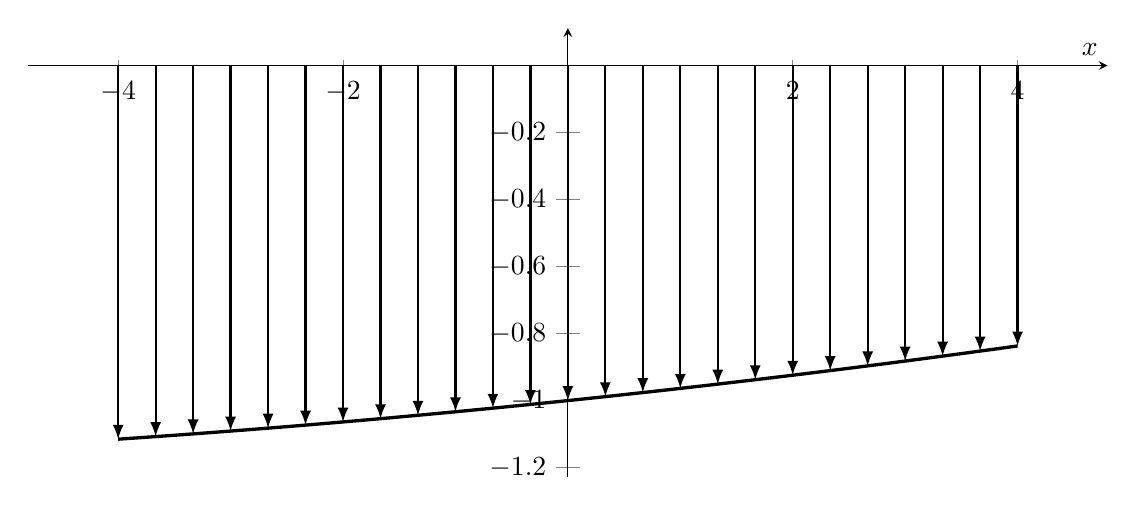
\begin{tikzpicture}
	\begin{axis}[axis lines=middle,no markers,enlargelimits,xscale=2,xtick={},ytick={},xlabel=$x$,
	]
	\addplot+[quiver={u=0,v=-y},latex-,black,thick,samples=25,domain=-4:4] {sin(2*x)-cos(pi*x)};
	\addplot[very thick,samples=200,smooth,domain=-4:4] {sin(2*x)-cos(pi*x)};
	\end{axis}\end{tikzpicture}
	\caption{Campionamento}
\end{figure}

Bisogna dimensionare il passo di campionamento $T$ al fine di avere un numero gestibile di campioni che consenta di ricostruire il segnale senza perdere informazione.

\subsection{Teorema del campionamento}
Per ricostruire fedelmente un segnale con spettro a banda limitata $[-B,B]$ su cui si è operato un campionamento a frequenza $f_S=\frac{1}{T}$ si deve avere $f_S\geq B$.
\begin{proof}[Dim.]
Dato il segnale $s(t)$ con spettro $S(f)$ limitato alle frequenze $f\in[-B,B]$ (in banda base), e data la proprietà dell'impulso di estrarre un campione del segnale, si definisce il segnale campionato $s_C(t)$ come il prodotto tra il segnale $s(t)$ e un treno di impulsi di ampiezza unitaria ad intervalli di tempo regolari di periodo $T$
\begin{equation}
s_C(t)=s(t)\cdot\sum_{n=-\infty}^{+\infty}{\impulse(t-n T)}
\end{equation}

Lo spettro del segnale campionato risulta essere dalla trasformata di Fourier la somma di tutte le repliche dello spettro del segnale di partenza $S(f)$ traslate a frequenze multiple di quella di campionamento
\begin{equation}
S_C(f)=S(f)\ast\fourier{\sum_{n=-\infty}^{+\infty}{\impulse(t-n T)}}=S(f)\ast\frac{1}{T}\sum_{n=-\infty}^{+\infty}{\f{\impulse}{f-\frac{n}{T}}}=\frac{1}{T}\sum_{n=-\infty}^{+\infty}{S(f-\frac{n}{T})}
\end{equation}

\begin{figure}[h!]
	\centering
	\subfloat[][$S(f)$]
	{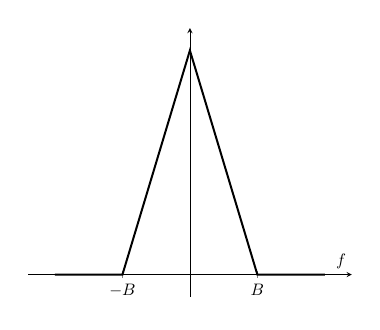
\begin{tikzpicture}[scale=.6]
		\begin{axis}[axis lines=middle,no markers,enlargelimits,xtick={-1,1},ytick={0},xticklabels={$-B$,$B$},xlabel={$f$}]
		\addplot [very thick]coordinates {(-2,0)(-1,0)(0,1)(1,0)(2,0)};
		\end{axis}\end{tikzpicture}}\qquad\subfloat[][$S_C(f)$] {
		\begin{tikzpicture}[scale=.6]
		\begin{axis}[axis lines=middle,no markers,enlargelimits,xscale=1.8,xtick={-3,-1,1,2,3,4},ytick={1},xticklabels={$-f_S$,$-B$,$B$,$f_S\!-\!B$,$f_S$,$f_S\!+\!B$},yticklabels={$\frac{1}{T}$},xlabel={$f$}]
		\addplot [very thick]coordinates {(-5,0)(-4,0)(-3,1)(-2,0)(-1,0)(0,1)(1,0)(2,0)(3,1)(4,0)(5,0)};
		\addplot [dashed] coordinates{(-1,0)(-1,1)(1,1)(1,0)};
		\end{axis}\end{tikzpicture}	
	}
	\caption{Esempio campionamento con $f_S\geq 2 B$}
\end{figure}\label{fig:campionamento}

Per poter ricostruire il segnale è necessario che le repliche spettrali del segnale campionato non si sovrappongano al segnale in banda base, fenomeno detto \textsc{aliasing}. Deve essere $f_S-B\geq B$ ovvero la frequenza di campionamento deve essere almeno il doppio della banda unilatera del segnale
\begin{equation}
f_S\geq 2 B
\end{equation}
o, equivalentemente, definita \textsc{frequenza di Nyquist} $f_N=f_S / 2$, il segnale di partenza può essere ricostruito se la sua banda unilatera è $B<f_N$.

\begin{figure}[!h]
\centering\begin{tikzpicture}[scale=.6]
\begin{axis}[axis lines=middle,no markers,enlargelimits,xscale=1.8,xtick={-1,.5,1,1.5,2.5},ytick={1},xticklabels={$-B$,$f_S\!-\!B$,$B$,$f_S$,$f_S\!+\!B$},yticklabels={$\frac{1}{T}$},xlabel={$f$}]
\addplot [very thick]coordinates {(-3,0)(-1,0)(0,1)(1,0)(3,0)};
\addplot [very thick,dashed]coordinates {(-3.5,0)(-2.5,0)(-1.5,1)(-.5,0)(.5,0)(1.5,1)(2.5,0)(3.5,0)};
\end{axis}\end{tikzpicture}	
\caption{Esempio aliasing, campionamento con $f_S<2 B$}
\end{figure}\label{fig:aliasing}
\end{proof}
\begin{esempio}
Un segnale audio con una banda $B=\SI{20}{\kilo\hertz}$ nella \textsc{Pulse Code Modulation (PCM)} viene campionato alle frequenze di $\SI{40}{\kilo\hertz}$ o $\SI{48}{\kilo\hertz}$.
\end{esempio}
\begin{nota}
Il segnale viene filtrato prima di essere campionato perché al segnale è sempre sovrapposto il rumore termico a tutte le frequenze.
\end{nota}
\begin{nota}
Se non è possibile campionare alla frequenza $f_S$ è necessario applicare un filtro di \emph{antialiasing} in una banda più stretta di $[-B,B]$, che fa perdere parte dell'informazione del segnale ma consente la ricostruzione seppur meno fedele del segnale originale.
\end{nota}

\subsection{Ricostruzione}

I campioni del segnale numerico giunti al ricevitore attraversano il \textsc{filtro di ricostruzione} per riottenere il segnale analogico di partenza. L'operazione di ricostruzione è necessaria per eliminare le repliche spettrali che non fanno parte dello spettro del segnale di partenza e che sono il risultato dell'operazione di campionamento.

Si utilizza un filtro passa basso ideale con banda pari alla frequenza di Nyquist, che faccia passare le frequenze comprese nell'intervallo $[-\frac{f_S}{2},\frac{f_S}{2}]$, e che compensi l'attenuazione di $\frac{1}{T}$ di $S_C(f)$, per l'eq.\ref{eq:filtro_passa_basso_ideale}
\begin{equation}
H(f)=T \rect{\frac{f}{f_S}}\qquad h(t)=\sinc{\frac{t}{T}}
\end{equation}

Il segnale ricostruito è la convoluzione del segnale campionato con il filtro
\begin{equation}\begin{split}
s_R(t)&=s_C(t)\ast h(t)=\intinf{s_C(\tau)h(t-\tau)}{\tau}=\\
&=\intinf{[s(\tau)\sum_{n=-\infty}^{+\infty}\impulse(\tau-n T)]\sinc{\frac{t-\tau}{T}}}{\tau}=\\
&=\intinf{\left[\sum_{n=-\infty}^{+\infty}s(n T)\impulse(\tau-n T)\right]\sinc{\frac{t-\tau}{T}}}{\tau}=\\
&=\intinf{\sum_{n=-\infty}^{+\infty}s(n T)\sinc{\frac{t-n T}{T}}\impulse(\tau-n T)}{\tau}=\\
\intertext{per la proprietà di setaccio dell'impulso l'integrale si riduce al valore in $\tau=n T$ si ha}
&=\sum_{n=-\infty}^{+\infty}s(n T)\sinc{\frac{t-n T}{T}}=\sum_{n=-\infty}^{+\infty}s(n T)\sinc{\frac{n T-t}{T}}
\end{split}
\end{equation}

Il segnale ricostruito nell'istante $t$ si ottiene come somma dei prodotti tra i campioni del segnale e il valore della funzione seno cardinale calcolata nei corrispondenti istanti di campionamento.

\begin{nota}
Se il segnale è passa banda, il teorema del campionamento continua a valere ma può essere impraticabile campionare al doppio della frequenza massima. In tal caso si sfruttano le repliche in banda base del segnale. Si seleziona una banda $B$ tale che la frequenza massima sia un multiplo intero della banda base, $\frac{f_M}{B}=m\in\N$, e si porrà $f_S\geq B$.
\end{nota}
\begin{nota}
Un campionamento perfetto dovrebbe estrarre l'informazione del segnale istantaneamente, mentre in realtà è necessario periodo di osservazione seppur breve. Un campionatore reale effettua la convoluzione del segnale con un rettangolo molto stretto, $s(t)\ast\rect{\frac{t}{\tau}}$ con un duty cycle molto piccolo, la cui trasformata risulta essere un $\Sinc$ molto ampio ($\frac{1}{\tau}\gg B$). Se in ricezione è richiesta alta fedeltà al segnale originale è sempre possibile equalizzare per compensare l'effetto sagomatore del filtro.
\end{nota}

\section{Quantizzazione}
L'operazione di \textsc{quantizzazione} trasforma i valori continui dei campioni del segnale appartenenti ad un intervallo $[-a,a]$ in valori discreti  dell'intervallo diviso in $Q$ livelli distinti di ampiezza $\Delta=\frac{2a}{Q}$.

Nei sistemi di elaborazione a logica binaria si assegna ad ogni campione del segnale un numero finito fisso di bit $N$ che consente di individuare $2^N$ livelli del segnale.

\begin{figure}[!h]
\centering
\begin{tikzpicture}
\begin{axis}[axis x line=middle,axis y line=left,enlargelimits,domain=-4:4,xlabel={$s(t)$},ylabel={$s_q(t)$},grid=major,xtick={-4,-3,-2,-1,0,1,2,3,4},ytick={-4,-3,-2,-1,0,1,2,3,4},extra y ticks={-3.5,-2.5,-1.5,-.5,0.5,1.5,2.5,3.5},extra y tick labels={$000$,$001$,$010$,$011$,$100$,$101$,$110$,$111$},extra y tick style={ticklabel pos=right}]
\addplot [const plot,very thick] coordinates {(-4,-3.5)(-3,-2.5)(-2,-1.5)(-1,-.5)(0,.5)(1,1.5)(2,2.5)(3,3.5)(4,3.5)};
\addplot [dashed] coordinates {(-4,-4)(4,4)};
\end{axis}
\end{tikzpicture}
\caption{Quantizzatore a 3 bit di segnale $s(t)\in[-4,4]$}
\end{figure}

L'operazione comporta una perdita di informazione irreversibile.

Dato un processo aleatorio stazionario il campionamento di una sua realizzazione $x(t)$ da luogo ad una variabile aleatoria, con la sua funzione densità di probabilità $f(x)$. Si supponga che la dinamica della v.a. assuma valori nell'intervallo $[-a,a]$, e che la quantizzazione in $Q$ livelli sia uniforme con intervalli di quantizzazione di ampiezza $\Delta=\frac{2a}{Q}$. I bordi degli intervalli si trovano in $x_i=-a+i\cdot\Delta$, con $i=0,\dots,Q$.  Per minimizzare l'errore di quantizzazione tra due intervalli successivi il livello assume valore intermedio
\begin{equation}
x_{i-1}\leq x<x_i,\,i=1,\dots,Q,\quad
x_q=\frac{x_i+x_i-1}{2}=-a+i\cdot\Delta-\frac{\Delta}{2}
\end{equation}
da cui risulta un errore di quantizzazione assoluto massimo di $\frac{\Delta}{2}$ in corrispondenza dei bordi degli intervalli.

L'operazione introduce quindi un rumore di quantizzazione che si può valutare con l'errore quadratico medio come
\[N_q=\E{(x-x_q)^2}=\intd{-a}{a}{(x-x_q)^2 f(x)}{x}=\sum_{i=1}^{Q}\intd{x_{i-1}}{x_i}{(x-x_q)^2 f(x)}{x}\]
Per un segnale con distribuzione uniforme si ha $f(x)=\frac{1}{2a},\,x\in[-a,a]$ e 0 altrove, da cui
\[\begin{split}N_q&=\sum_{i=1}^{Q}\intd{-a+(i-1)\Delta}{-a+i\Delta}{\left(x+a-i\Delta+\frac{\Delta}{2}\right)^2 \frac{1}{2a}}{x}=\\\intertext{ponendo $y=x+a-i\Delta+\frac{\Delta}{2}$}&=\frac{1}{2a}\sum_{i=1}^{Q}\intd{-\frac{\Delta}{2}}{\frac{\Delta}{2}}{y^2}{y}=\frac{Q}{2a}\bound{-\frac{\Delta}{2}}{\frac{\Delta}{2}}{\frac{y^3}{3}}=\frac{1}{\Delta}\frac{\Delta^3}{12}=\frac{\Delta^2}{12}
\end{split}\]
Tale quantità costituisce un disturbo che va confrontato con la potenza del segnale dato dallo spettro di potenza
\[S_x=\intd{-a}{a}{x^2\frac{1}{2a}}{x}=\frac{1}{2a}\bound{-a}{a}{\frac{x^3}{3}}=\frac{a^2}{3}=\frac{Q^2\Delta^2}{12}\]
Si ha il \textsc{rapporto segnale rumore di quantizzazione}
\begin{equation}
\frac{S_x}{N_q}=Q^2
\end{equation}
che migliora aumentando il numero di livelli di quantizzazione.
Per un numero di intervalli potenza di due si ha $\frac{S_x}{N_q}=2^{2n}$ che espresso in decibel \[\restrict{\frac{S_x}{N_q}}{\text{dB}}=10\Log 2^{2n}\cong n\cdot\SI{6}{\decibel}\]
ovvero si quadruplica il rapporto segnale rumore per ogni bit di quantizzazione in più.

Tale rapporto segnale rumore è stato calcolato per un processo con densità di probabilità uniforme, ma in generale la quantizzazione può essere non lineare, ad esempio per un processo gaussiano le cui realizzazioni si concentrano attorno al valor medio nullo e con varianza molto piccola. Per ottimizzare il rapporto segnale rumore di quantizzazione è necessaria una suddivisione più fine in livelli dove il segnale è più probabile, descrivendo i campioni con maggiore precisione.

\chapter[Teoria dell’informazione]{Principi di teoria dell’informazione e teorema di Shannon}
In un canale di comunicazione basato su un sistema di trasmissione numerico l'informazione viene trasformata nei blocchi di filtraggio, campionamento e quantizzazione in una sequenza di bit corrispondenti ad un alfabeto di $N$ simboli. In ricezione giunge in generale una sequenza di bit a cui sono associati $M$ simboli. In un canale di comunicazione ideale l'informazione viene trasmessa senza errori di trasmissione pertanto non è possibile scambiare un simbolo per un altro ($N=M$) per cui 
\[\begin{cases}
p(a_{i_R}|a_{i_T})=1 \\ p(a_{j_R}|a_{i_T})=0 \quad i\neq j
\end{cases}\]
Un canale binario può trasmettere e ricevere solo due simboli, ad esempio 0 e 1, emessi con probabilità $P(0_T)=P_0$ e $P(1_T)=P_1$. Ogni simbolo trasmesso può essere ricevuto correttamente con probabilità o con errore
\begin{figure}[!h]
\centering
\begin{tikzpicture}
\node (t0) {0};
\node [below= of t0](t1) {1};
\node [right of = t0,node distance=4cm](r0) {0};
\node [below= of r0](r1) {1};
\draw [-latex] (t0)--(r0) node[above,pos=.3] {$q_0$};
\draw [-latex] (t0)--(r1) node[above,pos=.3] {$p_0$};
\draw [-latex] (t1)--(r0) node[below,pos=.8] {$p_1$};
\draw [-latex] (t1)--(r1) node[below,pos=.8] {$q_1$};
\end{tikzpicture}
\end{figure}

\[\begin{cases}
q_0=P(0_R|0_T)& \text{prob. trasmissione corretta simbolo 0}\\ p_0=P(1_R|0_T)&\text{prob. trasmissione errata simbolo 0}\\ q_0+p_0=1\\
q_1=P(1_R|1_T)& \text{prob. trasmissione corretta simbolo 1}\\ p_1=P(0_R|1_T)& \text{prob. trasmissione errata simbolo 1} \\ q_1+p_1=1
\end{cases}\]

Si ha un \textsc{canale binario simmetrico} quando la probabilità di errore o \textsc{Bit Error Rate} non distingue i due simboli  $p_0=p_1=\text{BER}$

La probabilità di errore per trasmissione su un canale binario 
\[ P(E)=P(E\cap 0_T)+P(E\cap 1_T)=P(1_R|0_T)P(0_T)+P(0_R|1_T)P(1_T)=p_0 P_0+p_1 P_1 \]

Se il canale è binario simmetrico
\[P(E)=\text{BER}\cdot(P_0+P_1)=\text{BER}\]

Le probabilità di ricevere i due simboli
\[P(0_R)=P(0_R|0_T)P(0_T)+P(0_R|1_T)P(1_T)=q_0 P_0+p_1 P_1\]
\[P(1_R)=P(1_R|0_T)P(0_T)+P(1_R|1_T)P(1_T)=p_0 P_0+q_1 P_1\]



\begin{figure}[!h]
	\begin{center}\begin{tikzpicture}[node distance=.5cm]
		\node [draw,circle] (S) {S};
		\node [block, right= of S,text width=2cm] (cs) {codifica sorgente};
		\node [block, right=of cs,text width=2cm] (cc) {codifica canale};
		\node [block,right=of cc,text width=2cm, minimum height=.5cm,node distance=2cm] (c) {canale};
		\node [block, right=of c,text width=2cm] (dc) {decodifica canale};
		\node [draw, dashed, fit=(cc)(c)(dc), rounded corners, inner sep=2mm] {};
		\node [block, right=of dc,text width=2cm] (ds) {decodifica sorgente};
		\node [draw,circle,right=of ds] (R) {R};		
		\draw [-latex] (S) -- (cs);
		\draw [-latex] (cs) -- (cc);
		\draw [-latex] (cc) -- (c);
		\draw [-latex] (c) -- (dc);
		\draw [-latex] (dc) -- (ds);
		\draw [-latex] (ds) -- (R);		
		\end{tikzpicture}
	\end{center}
\caption{Schema a blocchi di trasmissione numerica}
\end{figure}

\section{Codifica di sorgente}
L'errore sul canale binario può essere ridotto ricorrendo alla \textsc{codifica di sorgente} che trasforma i simboli generati dalla sorgente in una sequenza di bit che possa risolvere o ridurre alcuni problemi causati dalla trasmissione su canale rumoroso.

La codifica di canale è la parte del sistema che trasforma la sequenza di bit in forme d'onda adattate al mezzo trasmissivo.

In ricezione si eseguono le operazioni contrarie per riottenere l'informazione trasmessa.

\subsection{Codice a ripetizione}
Una codifica di sorgente è il \textsc{codice a ripetizione} per un canale binario simmetrico. Ogni bit generato dalla sorgente viene ripetuto $2n+1$ volte, il che riduce la velocità di trasmissione (\emph{bit rate}) dello stesso fattore. Il ricevitore interpreta la sequenza di $2n+1$ bit come il bit che si è presentato in maggioranza. Questo consente in ricezione di rilevare e correggere fino a $n$ errori. La sequenza è interpretata erroneamente se sono errati la maggioranza dei bit, ovvero almeno $n+1$. 

La sequenza di bit in ricezione può essere assimilata ad un processo di Bernoulli, con due simboli che arrivano indipendentemente l'uno dall'altro. La probabilità di errore è data da tutte le combinazioni che hanno tra $n+1$ e $2n+1$ bit errati, ovvero
\[p(E)=\sum_{k=n+1}^{2n+1}\binom{2n+1}{k}p^k(1-p)^{2n+1-k}\]

\begin{esempio}
Dato un canale di trasmissione binario con probabilità di errore sul bit $p=10^{-3}$, si vuole dimensionare un codice a ripetizione tale da avere una probabilità di errore $p(E)=10^{-9}$.
Con la formula di Bernoulli si può approssimare con una stima per difetto la probabilità di errore con \[\binom{2n+1}{n+1}p^{n+1}(1-p)^n=\frac{(2n+1)!}{(n+1)!n!}\,p^{n+1}(1-p)^n\]
con $n=1$ si ha $p(E)=\frac{3!}{2!1!}(10^{-3})^2(1-10^{-3})\cong 10^{-6}$\\
con $n=2$ si ha $p(E)=\frac{5!}{3!2!}(10^{-3})^3(1-10^{-3})^2\cong 10^{-8}$\\
\end{esempio}

\subsection{Codice a controllo di parità}
Nella codifica di sorgente \textsc{a controllo di parità} si aggiunge alla stringa di bit da trasmettere un bit di parità. In una codifica a parità pari ci si assicura che la stringa di $n$ bit contenga un numero pari di bit uguali ad 1.

Se il canale di trasmissione introduce un errore su un bit con probabilità $p$ il ricevitore rivela la parità errata. In generale il ricevitore può rivelare un numero dispari di errori.
La probabilità di avere un numero dispari di errori è
\[p(R)=\sum_{k=1}^{n/2}\binom{n}{2k-1}\,p^{2k-1}(1-p)^{n-2k+1}\]

Il ricevitore non può rivelare l'errore in caso di un numero pari di errori, il che si verifica con probabilità
\[p(E_{NR})=\sum_{k=1}^{n/2}\binom{n}{2k}\,p^{2k}(1-p)^{n-2k}\]

La probabilità che la trasmissione della stringa di $n$ bit sia corretta è
\[p(C)=(1-p)^n\]

Date le tre alternative si ha
\[p(R)+p(E_{NR})+p(C)=1\]

Il ricevitore può chiedere la ritrasmissione della stringa di $n$ bit quando rivela la parità errata.
Se il ricevitore continua a chiedere la ritrasmissione sino a che non rivela un errore si ha una probabilità di errore totale
\[p(E)=p(E_{NR})+p(R)p(E_{NR})+p(R)^2p(E_{NR})+\dots=p(E_{NR})\cdot\sum_{k=0}^{\infty}p(R)^k=\frac{p(E_{NR})}{1-p(R)}\]

Il numero di ritrasmissioni è una variabile casuale.
La ritrasmissione non è necessaria se la trasmissione è corretta o si verificano uno o più errori non rivelabili, con probabilità \[p(n_R=0)=p(E_{NR})+p(C)=1-p(R)\]

\`{E} necessaria $k$ volte con probabilità \[p(n_R=k)=[1-p(R)]p(R)^k\]

Il numero medio di ritrasmissioni
\[\E{n_R}=\sum_{k=0}^{\infty}k\cdot p(n_R=k)=\sum_{k=0}^{\infty}k\cdot[1-p(R)]p(R)^k=\frac{p(R)}{1-p(R)}\]

Il numero medio di trasmissioni compressa la prima è $n_T=1+n_R$:
\[\E{n_T}=1+\E{n_R}=\frac{1}{1-p(R)}\]
La probabilità di ricezione corretta complessiva considerato il caso con ritrasmissioni
\[p(C_T)=p(C)+p(R)p(C)+p(R)^2p(C)+\dots=p(C)\cdot\sum_{k=0}^{\infty}p(R)^k=\frac{p(C)}{1-p(R)}\]

\begin{esempio}
Dato un canale di trasmissione binario con probabilità di errore sul bit $p=10^{-3}$, si vuole dimensionare un codice a ripetizione tale da avere una probabilità di errore $p(E)=10^{-9}$.

Si da una stima approssimata di errore non rilevato per il caso più probabile di doppio errore di trasmissione
\[p(E_{NR})\cong\binom{n}{2}p^2(1-p)^2=\frac{n!}{2!(n-2)!}\cdot 10^{-6}\]
Non è possibile ridurre il \emph{bit error rate} al di sotto di tale stima ed avere un $\text{BER}\leq 10^{-9}$ 
\end{esempio}

\section{Teoria dell'informazione}
Dato un canale di comunicazione basato su un sistema di trasmissione è importante quantificare il limite teorico di informazione trasmissibile (\textsc{Shannon}, 1948). \`{E} fondamentale poter confrontare i sistemi reali affetti da rumore gaussiano rispetto ad un sistema teorico, che astrae i dettagli implementativi e fissa un limite teorico di efficienza del sistema di trasmissione.

Nel modello l'informazione viene generata da una sorgente che emette, a velocità costante e incorrelati tra loro, $m$ simboli $x_1,x_2,\dots,x_m$ scelti da un alfabeto. Un legge di codifica associa ad ogni simbolo una sequenza di bit. Per rappresentare $m$ simboli di un alfabeto sono necessari $\log_2 m$ bit/simbolo.

Ogni simbolo $x_i$ può occorrere con una certa probabilità $p_i=p(x_i)$ ed essere rappresentato con una stringa di $n_i$ bit.
Se i simboli sono equiprobabili è ragionevole una codifica a lunghezza fissa. Se i simboli non sono equiprobabili è ragionevole attribuire stringhe di bit più corte ai simboli più probabili.

La quantità di informazione media che transita sul canale sarà quindi una media pesata delle lunghezze in bit dei simboli per la probabilità dei simboli: \[\sum_{i}p_i\cdot n_i\]

Nel caso di una sorgente ergodica è possibile derivare le statistiche del processo dall'osservazione di una singola realizzazione. In un messaggio costituito da una sequenza di $N$ simboli, con $N$ grande, ogni simbolo $x_i$ si presenterà mediamente $n_i=p_i N$ volte. Con questi $N$ simboli si possono costruire numerosi messaggi che rispettino tali statistiche di sorgente e che si differenziano tra loro per la posizione dei simboli all'interno del messaggio. La probabilità di generare un messaggio lecito è
\begin{equation}p_\text{mess}=p_1^{p_1 N}\cdot p_2^{p_2 N}\cdot\dots\cdot p_m^{p_m N}\end{equation}
Per una sorgente ergodica ogni messaggio lecito di lunghezza $N$ è equiprobabile, essendo i simboli emessi in modo indipendente il particolare ordine di emissione non è importante, quindi tutti i possibili messaggi leciti con $N$ simboli sono proprio $1/p_\text{mess}$.
Per rappresentare quindi un tal numero di messaggi leciti sono necessari un numero di bit di informazione pari a
\[n=\log_2\frac{1}{p_\text{mess}}=-\log_2 p_\text{mess}\]
e quindi il numero medio di bit per simbolo generato dalla sorgente S, anche detta \textsc{entropia della sorgente}
\begin{equation}\begin{split}
H(S)=\frac{n}{N}&=\frac{1}{N}\log_2\frac{1}{p_\text{mess}}=-\frac{1}{N}\log_2 p_\text{mess}=\\
&=-\frac{1}{N}\log_2\prod_{i=1}^{m}p_i^{N p_i}=-\frac{1}{N}\sum_{i=1}^{m}\log_2 p_i^{N p_i}=\\
&=-\sum_{i=1}^{m}p_i\log_2 p_i
\end{split}\end{equation}
La quantità $I(x_i)=-\log_2 p(x_i)$ rappresenta il minimo numero di bit necessari per descrivere il simbolo $x_i$ e quindi una misura dell'informazione associata al simbolo. Quanto più probabile è l'emissione di un simbolo tanto meno informazione esso trasporta. Si possono riassumere le seguenti proprietà per l'informazione associata alla sorgente:
\begin{enumerate}
\item L'emissione di un simbolo come evento certo non contiene alcuna informazione \[p(x_i)=1 \iff I(x_i)=0\]
\item Vi è maggiore informazione associata ad un simbolo meno probabile \[I(x_i)>I(x_j)\iff p(x_i)<p(x_j)\]
\item Per coppie di simboli emessi in modo indipendente si ha
\[P(x_i,x_j)=p(x_i)\cdot p(x_j)\implies I(x_i,x_j)=I(x_i)+I(x_j)\]
infatti $I(x_i,x_j)=\log_2\frac{1}{p(x_i,x_j)}=\log_2\frac{1}{p(x_1)p(x_2)}=\log_2\frac{1}{p(x_i)}+\log_2\frac{1}{p(x_j)}=I(x_i)+I(x_j)$
\item Dato un alfabeto di $M$ simboli, l'entropia della sorgente verifica la disuguaglianza
\begin{equation}H(S)\leq\log_2 M\end{equation}
\begin{proof}
\[H(S)-\log_2 M\leq 0\]
\[\sum_{i=1}^{M}p_i\log_2\frac{1}{p_i}-\log_2 M\leq 0\]
sviluppando il primo membro, ed essendo $\sum_i p_i=1$
\[\sum_{i=1}^{M}p_i\log_2\frac{1}{p_i}-\sum_{i=1}^{M}p_i\log_2 M=\sum_{i=1}^{M}p_i\left[\log_2\frac{1}{p_i}-\log_2 M\right]=\sum_{i=1}^{M}p_i\log_2\frac{1}{p_i M}\]
che è possibile maggiorare essendo $\log y\leq y-1$
\[\leq \sum_{i=1}^{M}p_i\left(\frac{1}{p_i M}-1\right)\log_2\e{}= \sum_{i=1}^{M}\left(\frac{1}{M}-p_i\right)\log_2\e{}=0\]
\end{proof}

\begin{esempio}
Nel caso di sorgente con $M$ simboli equiprobabili si ha
\[p_i=p=\frac{1}{M}\qquad I(x)=\log_2\frac{1}{M}\]
L'entropia della sorgente
\[H(S)=\sum_{i=1}^{M}p_i I(x_i)=-\sum_{i=1}^{M}\frac{1}{M}\log_2\frac{1}{M}=\log_2 M\]
assume il valore massimo teorico con l'uguaglianza $H(S)=\log_2 M$.
\end{esempio}
\begin{esempio}
Nel caso di sorgente binaria con 2 simboli con probabilità $p_0=p$ e $p_1=1-p$ si ha l'entropia
\[H(S)=-p\log_2 p-(1-p)\log_2(1-p)\]

\begin{figure}[h!]
	\centering\begin{tikzpicture}[scale=.6]
	\begin{axis}[axis lines=middle,no markers,enlargelimits,xtick={0.5,1},xticklabels={$\frac{1}{2}$,$1$},ytick={1},xlabel={$p$},ylabel={$H(S)$},xscale=2]
	\addplot [thick,domain=0:1] { -x*ln(x)/ln(2)-(1-x)*ln(1-x)/ln(2) };
	\end{axis}\end{tikzpicture}
	\caption{Entropia di una sorgente binaria}
\end{figure}
\end{esempio}
\end{enumerate}

\section{Sorgente con memoria}
Una sorgente può emettere simboli che non siano statisticamente indipendenti tra loro. La definizione di entropia della sorgente deve tener conto dell'informazione associata alla dipendenza statistica fra simboli.

L'informazione legata all'emissione del simbolo $x_1$ condizionata all'emissione di un simbolo precedente $x_0$:
\[I(x_1|x_0)=-\log_2(x_1|x_0)\]

L'entropia della sorgente, ovvero l'informazione media per simbolo generato da sorgente con memoria, condizionata all'emissione di un simbolo $x_0$ risulta
\[H(S|x_0)=\sum_i p(x_i|x_0) I(x_i|x_0) = -\sum_i p(x_i|x_0)\log_2 p(x_i|x_0)\]

\`{E} possibile definire l'informazione media o entropia del primo ordine considerando la media pesata di tutte le possibili emissioni di simboli precedenti. Per estensione si può supporre una sorgente con memoria più estesa e dipendenza tra più simboli in sequenza.

\section{Teorema di Shannon}
Si definisce la \textsc{capacità del canale} trasmissivo la misura dell'informazione che il canale è in grado di far transitare, ovvero alla quantità di bit nell'unità di tempo che riescono a transitare correttamente sul canale.

Su un canale reale i simboli in uscita dal mezzo trasmissivo sono affetti da errori, l'entropia del canale contiene anche informazione errata a causa degli errori di trasmissione.

Dato un canale affetto da errore di tipo gaussiano, a media nulla e data varianza, si ha che la capacità del canale, calcolata in bit/s,
\begin{equation}
C=B \log_2 \left(1+\frac{S}{N}\right)
\end{equation}

Tale risultato, noto come \textsc{teorema di Shannon}, permette di stabilire un limite superiore alla capacità di trasmettere bit sul canale, dato il rapporto tra potenza statistica del segnale sorgente $S$ e potenza statistica del rumore di canale $N$.

\begin{nota}
\`{E} possibile aumentare il rapporto segnale/rumore incrementando la potenza del segnale trasmesso o riducendo il rumore sul canale (ad esempio avvicinando Tx e Rx o modificando la tecnologia del mezzo trasmissivo).
\end{nota}

\chapter*{Appendice}
\begin{table*}[!h]
\centering
\caption{Variabili aleatorie}
\begin{tabular}{cccccc}
\hline \rule[-2ex]{0pt}{5.5ex} v.a. & $f_X(x)$\quad\tablefootnote{funzione probabilità di massa per v.a. discrete $f_X(x)=\sum_k p_k\impulse(x-k)$} & $\mu_X$ & $\E{X^2}$ & $\sigma^2_X$ & $G_X(t)$\quad\tablefootnote{funzione generatrice dei momenti} \\ 
\hline \rule[-2ex]{0pt}{5.5ex} uniforme & $\frac{1}{b-a}$ & $\frac{b+a}{2}$ & $\frac{b^2+ab+a^2}{3}$ & $\frac{(b-a)^2}{12}$ \\ 
\hline \rule[-2ex]{0pt}{5.5ex} esponenziale & $\lambda\e{-\lambda x}\step(x)$ & $\frac{1}{\lambda}$ & $\frac{2}{\lambda^2}$ & $\frac{1}{\lambda^2}$\\
\hline \rule[-2ex]{0pt}{5.5ex} disc. Poisson & $\frac{(\Lambda T)^k}{k!}\e{-\Lambda T}$ & $\Lambda T$ & $(\Lambda T)^2+\Lambda T$ & & $\e{-\Lambda T}\e{\Lambda T\e{t}}$ \\
\hline \rule[-2ex]{0pt}{5.5ex} disc. Bernoulli & $\binom{n}{k}p^k(1-p)^{n-k}$ & $n p$ & $n p [p(n-1)+1]$ & $n p(1-p)$ & $(p\e{t}+1-p)^n$ \\
\hline \rule[-2ex]{0pt}{5.5ex} disc. geometrica & $p^k(1-p)$ & $\frac{p}{1-p}$ & $\frac{p(1-p)}{(1-p)^2}$ & $\frac{p}{(1-p)^2}$ & $(1-p)(1-p\e{t})^{-1}$ \\
\hline \rule[-2ex]{0pt}{5.5ex} gaussiana & $\frac{1}{\sqrt{2\pi\sigma^2_X}}\;\e{-\tfrac{(x-\mu_X)^2}{2\sigma^2_X}}$ & $\mu_X$ & $\mu^2_X+\sigma^2_X$ & $\sigma^2_X$ & $\e{t\mu_X+\frac{\sigma^2_X t^2}{2}}$
\end{tabular}
\end{table*}